
\documentclass[11pt,letterpaper]{article}

\usepackage[margin=1in]{geometry}
\usepackage[utf8]{inputenc}

\usepackage{cite}
\usepackage[bookmarks=true,pdfstartview=FitH,colorlinks,linkcolor=darkred,filecolor=darkred,citecolor=darkred,urlcolor=darkred]{hyperref}


\usepackage{multicol}
\usepackage{color,xcolor}
\usepackage{graphicx,color,eso-pic}
\usepackage{amsmath,amssymb,stmaryrd}
\usepackage{boxedminipage}
\usepackage{cite}
\usepackage{url}
\usepackage{graphicx}
\usepackage[bf]{caption}
\usepackage{subcaption}
\usepackage{color}
\usepackage{xspace}
\usepackage{multirow}
\usepackage{amsmath,amsthm,amstext,amssymb,amsfonts,latexsym}
\usepackage{wrapfig}
\usepackage{comment}
\usepackage{algorithmicx}
 \usepackage{algpseudocode}



\definecolor{darkred}{rgb}{0.5, 0, 0}
\definecolor{darkgreen}{rgb}{0, 0.5, 0}
\definecolor{darkblue}{rgb}{0,0,0.5}

\newcommand{\gnote}[1]{{\footnotesize\color{red}[Gilad: #1]}}


\newenvironment{proofof}[1]{\noindent \textbf{Proof of #1:}}{\hfill \qed}



\newtheorem{thm}{Theorem}[section]      % A counter for Theorems etc
\newtheorem{theorem}[thm]{Theorem}
\newtheorem{conjecture}[thm]{Conjecture}
\newtheorem{lemma}[thm]{Lemma}
\newtheorem{claim}[thm]{Claim}
\newtheorem{corollary}[thm]{Corollary}
\newtheorem{fact}[thm]{Fact}
\newtheorem{proposition}[thm]{Proposition}
\newtheorem{example}[thm]{Example}


%{
%\theoremstyle{definition}
\newtheorem{definition}[thm]{Definition}
\newtheorem{remark}[thm]{Remark}
%}


\newtheoremstyle{boxes}% name  
{2pt}% ?Space above ? 
{0pt}% ?Space below ?
{}% ?Body font ?
{}% ?Indent amount ?
{\bfseries}% ?Theorem head font?
{}% ?Punctuation after theorem head ?
{\newline}% ?Space after theorem head ?
{\thmname{#1}\thmnumber{ #2}:  
\thmnote{#3}}

\theoremstyle{boxes}
\newtheorem{algorithm}[thm]{Algorithm}%{\bf}{} %
\newtheorem{myalgo}[thm]{Algorithm}%{\bf}{} %
\newtheorem{myfunc}[thm]{Functionality}%{\bf}{} %
\newtheorem{myconst}[thm]{Construction}%{\bf}{} %

\newcommand{\algo}[3]{
\medskip
\noindent\begin{minipage}{\textwidth}
\rule{\linewidth}{0.3mm}
\begin{myalgo}
[\sloppy {#1}\vspace{-1.5ex}]\label{#2}\vspace{-1ex}
\rule{\linewidth}{0.1mm}
\end{myalgo}
\end{minipage}
%\vspace{-1.5ex}
%\leavevmode\vspace{-1.2\baselineskip}
{#3}
%\vspace{-2.7ex}
\noindent
\rule{\linewidth}{0.3mm}
}

\newcommand{\func}[3]{
\medskip
\noindent\begin{minipage}{\textwidth}
\rule{\linewidth}{0.3mm}
\begin{myfunc}
[\sloppy {#1}\vspace{-1.5ex}]\label{#2}\vspace{-1ex}
\rule{\linewidth}{0.1mm}
\end{myfunc}
\end{minipage}
%\vspace{-1.5ex}
%\leavevmode\vspace{-1.2\baselineskip}
{#3}
\vspace{-2.7ex}
\noindent
\rule{\linewidth}{0.3mm}
}

\newcommand{\const}[3]{
\medskip
\noindent\noindent\begin{minipage}{\textwidth}
\rule{\linewidth}{0.3mm}
\begin{myconst}
[\sloppy {#1}\vspace{-1.5ex}]\label{#2}\vspace{-1ex}
\rule{\linewidth}{0.1mm}
\end{myconst}
\end{minipage}
%\vspace{-1.5ex}
%\leavevmode\vspace{-1.2\baselineskip}
{#3}

\vspace{-2.7ex}
\noindent
\rule{\linewidth}{0.3mm}
}

\newcommand{\eqdef}{\stackrel{\rm def}{=}}
\newcommand{\indist}{\stackrel{\rm c}{\equiv}}
\newcommand{\statclose}{\stackrel{\rm s}{\equiv}}


\newenvironment{MyEnumerate}[1]{\begin{enumerate}\setlength{\itemsep}{0.1cm}
\setlength{\parskip}{-0.05cm} #1}{\end{enumerate}}
\newenvironment{MyItemize}[1]{\begin{itemize}\setlength{\itemsep}{0.1cm}
\setlength{\parskip}{-0.05cm} #1}{\end{itemize}}

\renewcommand{\sec}{{\lambda}}
\newcommand{\A}{{\cal A}}
\renewcommand{\S}{{\cal S}}
\newcommand{\bit}{{\{0,1\}}}



\newcommand{\X}{\mathbf{X}}
\renewcommand{\sec}{{\lambda}}
\newcommand{\e}{{\epsilon}}

\newcommand{\bsize}{\ensuremath{b}}
\newcommand{\op}{\ensuremath{\mathsf{op}}\xspace}
\newcommand{\data}{{\ensuremath{\mathsf{data}}}\xspace}
\newcommand{\addr}{{\ensuremath{\mathsf{addr}}}\xspace}

\newcommand{\Sim}{\ensuremath{{\sf Sim}}\xspace}
\newcommand{\abs}[1]{\left|{#1}\right|}





%\newcommand{\data}{{\ensuremath{\mathsf{data}}}\xspace}
%\newcommand{\wdata}{{\mathsf{wdata}}}
%\newcommand{\fetched}{{\mathsf{rdata}}}


\newcommand{\cpu}{\ensuremath{\text{CPU}}\xspace}
\newcommand{\cpus}{\ensuremath{\text{CPUs}}\xspace}

\newcommand{\mem}{{\ensuremath{\mathsf{mem}}}\xspace}
\newcommand{\add}{{\ensuremath{\mathsf{addr}}}\xspace}

\newcommand{\Read}{{\ensuremath{\mathsf{read}}}\xspace}
\newcommand{\Write}{{\ensuremath{\mathsf{write}}}\xspace}
\newcommand{\pos}{{\ensuremath{\mathsf{pos}}}\xspace}
\newcommand{\opram}{{\ensuremath{\mathsf{OPRAM}}}\xspace}



\newcommand{\flag}{{\sf flag}\xspace}
\newcommand{\dummy}{{\sf dummy}\xspace}



%\sloppy
%\widowpenalty10000
%\clubpenalty10000

\begin{document}

\title{\bf Bucket Oblivious Sort: \\An Extremely Simple Oblivious Sort\thanks{The paper was presented in the 3rd Symposium on Simplicity in Algorithms, SOSA@SODA 2020. This version is identical
to the SOSA'20 conference version modulo typo corrections.
}}

\author{Gilad Asharov \thanks{Bar-Ilan University. Part of the work was done while the author was a post-doctoral fellow at Cornell Tech supported a Junior Fellow award from the Simons Foundation, and while at J.P. Morgan AI Research.} \qquad
T-H. Hubert Chan\thanks{The University of Hong Kong. Partially supported the Hong Kong RGC under the grant 17200418.} \qquad
Kartik Nayak\thanks{Duke University. Part of the work was done while the author was at University of Maryland.} \\
Rafael Pass\thanks{Cornell Tech.} \qquad
Ling Ren\thanks{University of Illinois Urbana-Champaign. Part of the work was done while the author was at MIT.} \qquad
Elaine Shi\thanks{Cornell University.}}

\newcommand{\rl}[1]{{\footnotesize\color{orange}[Ling: #1]}}

\date{}

\maketitle

%\fancyfoot[R]{\scriptsize{Copyright \textcopyright\ 2020 by SIAM\\
%Unauthorized reproduction of this article is prohibited}}

\begin{abstract}
We propose a conceptually simple oblivious sort and oblivious random permutation algorithms called bucket oblivious sort and bucket oblivious random permutation.
Bucket oblivious sort uses $6n\log n$ time (measured by the number of memory accesses) and $2Z$ client storage to ensure an error probability exponentially small in $Z$. 
This runtime is only $3\times$ slower than a non-oblivious merge sort baseline;
for $2^{30}$ elements, it is $5\times$ faster than Bitonic sort,
the de facto oblivious sorting algorithm in practical implementations. 
%We thus recommend our algorithms as an attractive alternative to Bitonic Sort.

%Finally, we show that using our Bucket Sort as a meta-algorithm and leveraging additional algorithmic tricks,
%we can devise a new ``locality-friendly'' oblivious sorting algorithm that outperforms the state of the art (Asharov et al., Eurocrypt 2019) by an almost logarithmic factor in both runtime and locality.

% and $\widetilde{O}(\log n)$ depth
%%% Local Variables:
%%% mode: plain-tex
%%% TeX-master: "main"
%%% End:

\end{abstract}

%!TEX root = main.tex


%\gnote{Write the paper in the client-server model, where the client can hold $4$ buckets at a time; Write the introduction as such; Move all other optimizations to "extensions"}

\section{Introduction}

With the increased use of outsourced storage and computation, privacy of the outsourced data has been of paramount importance. 
A canonical setting is where a client with a small local
storage outsources its encrypted data to an untrusted server. 
In this setting, encryption alone is not sufficient to preserve privacy.
The access patterns to the data may reveal sensitive information. 

Two fundamental building blocks for oblivious storage and computation~\cite{goldreich1996software,goodrich2011privacy,oblivistore} are oblivious sorting and oblivious random permutation.
In these two problems, an array of $n$ elements is stored on an untrusted server, encrypted under a trusted client's secret key.
The client wishes to sort or permute the $n$ elements in a \emph{data-oblivious} fashion.
That is, the sequence of accesses it makes to the server should not reveal any information about the $n$ elements (e.g., their relative ranking).
The client has a small amount of local storage, the access pattern to which cannot be observed by the server.
This work presents simple and efficient algorithms to these two problems, named bucket oblivious sort and bucket oblivious random permutation.

\subsection{State of the Affairs.}
For oblivious sort, it is well-known that one can leverage 
sorting networks such as AKS~\cite{aks} and Zig-zag sort~\cite{zigzag}
to obliviously sort $n$ elements in $O(n\log n)$ time. 
Unfortunately, these algorithms are complicated and incur enormous constants rendering them completely impractical. 
%\rl{What's expensive is approximate halvers, not expanders.} 
Thus, almost all known practical implementations~\cite{oblivistore,oblivm,graphsc}
instead employ the simple bitonic sort algorithm~\cite{bitonic}. 
While asymptotically worse, due to the small leading constants, bitonic sort performs much better in practice.

Oblivious random permutation (ORP) can be realized by assigning a sufficiently long random key to each element, and then obliviously sorting the elements by the keys.
To the best of our knowledge, this remains the most practical solution for ORP.
It then follows that while $O(n \log n)$ algorithms exist in theory, practical instantiations resort to the $O(n \log^2 n)$ bitonic sort.
There exist algorithms such as the Melbourne
shuffle~\cite{ohrimenko2014melbourne} that do not rely on
oblivious sort; but they require $O(\sqrt{n})$ client storage to permute $n$ elements.
Other approaches include the famous Thorp shuffle~\cite{thorp01} and random permutation networks~\cite{randpermnet}, but none of these solutions are competitive in performance either asymptotically or concretely.

\subsection{Our Results.}
Let $Z$ be a statistical security parameter that controls the error probability. 
Our bucket oblivious sort runs in $6n\log n$ time ($4n\log n$ for bucket ORP) and has an error probability around $e^{-Z/6}$ when the client can store $2Z$ elements locally.
This is at most $3\times$ slower than the non-oblivious merge sort, and is at least $5\times$ faster than bitonic sort for $n=2^{30}$ (cf. Table~\ref{tab:compare}).
Therefore, we recommend bucket oblivious sort and bucket ORP as attractive alternatives to bitonic sort in practical implementations.

\begin{figure*}[h!]
\centering
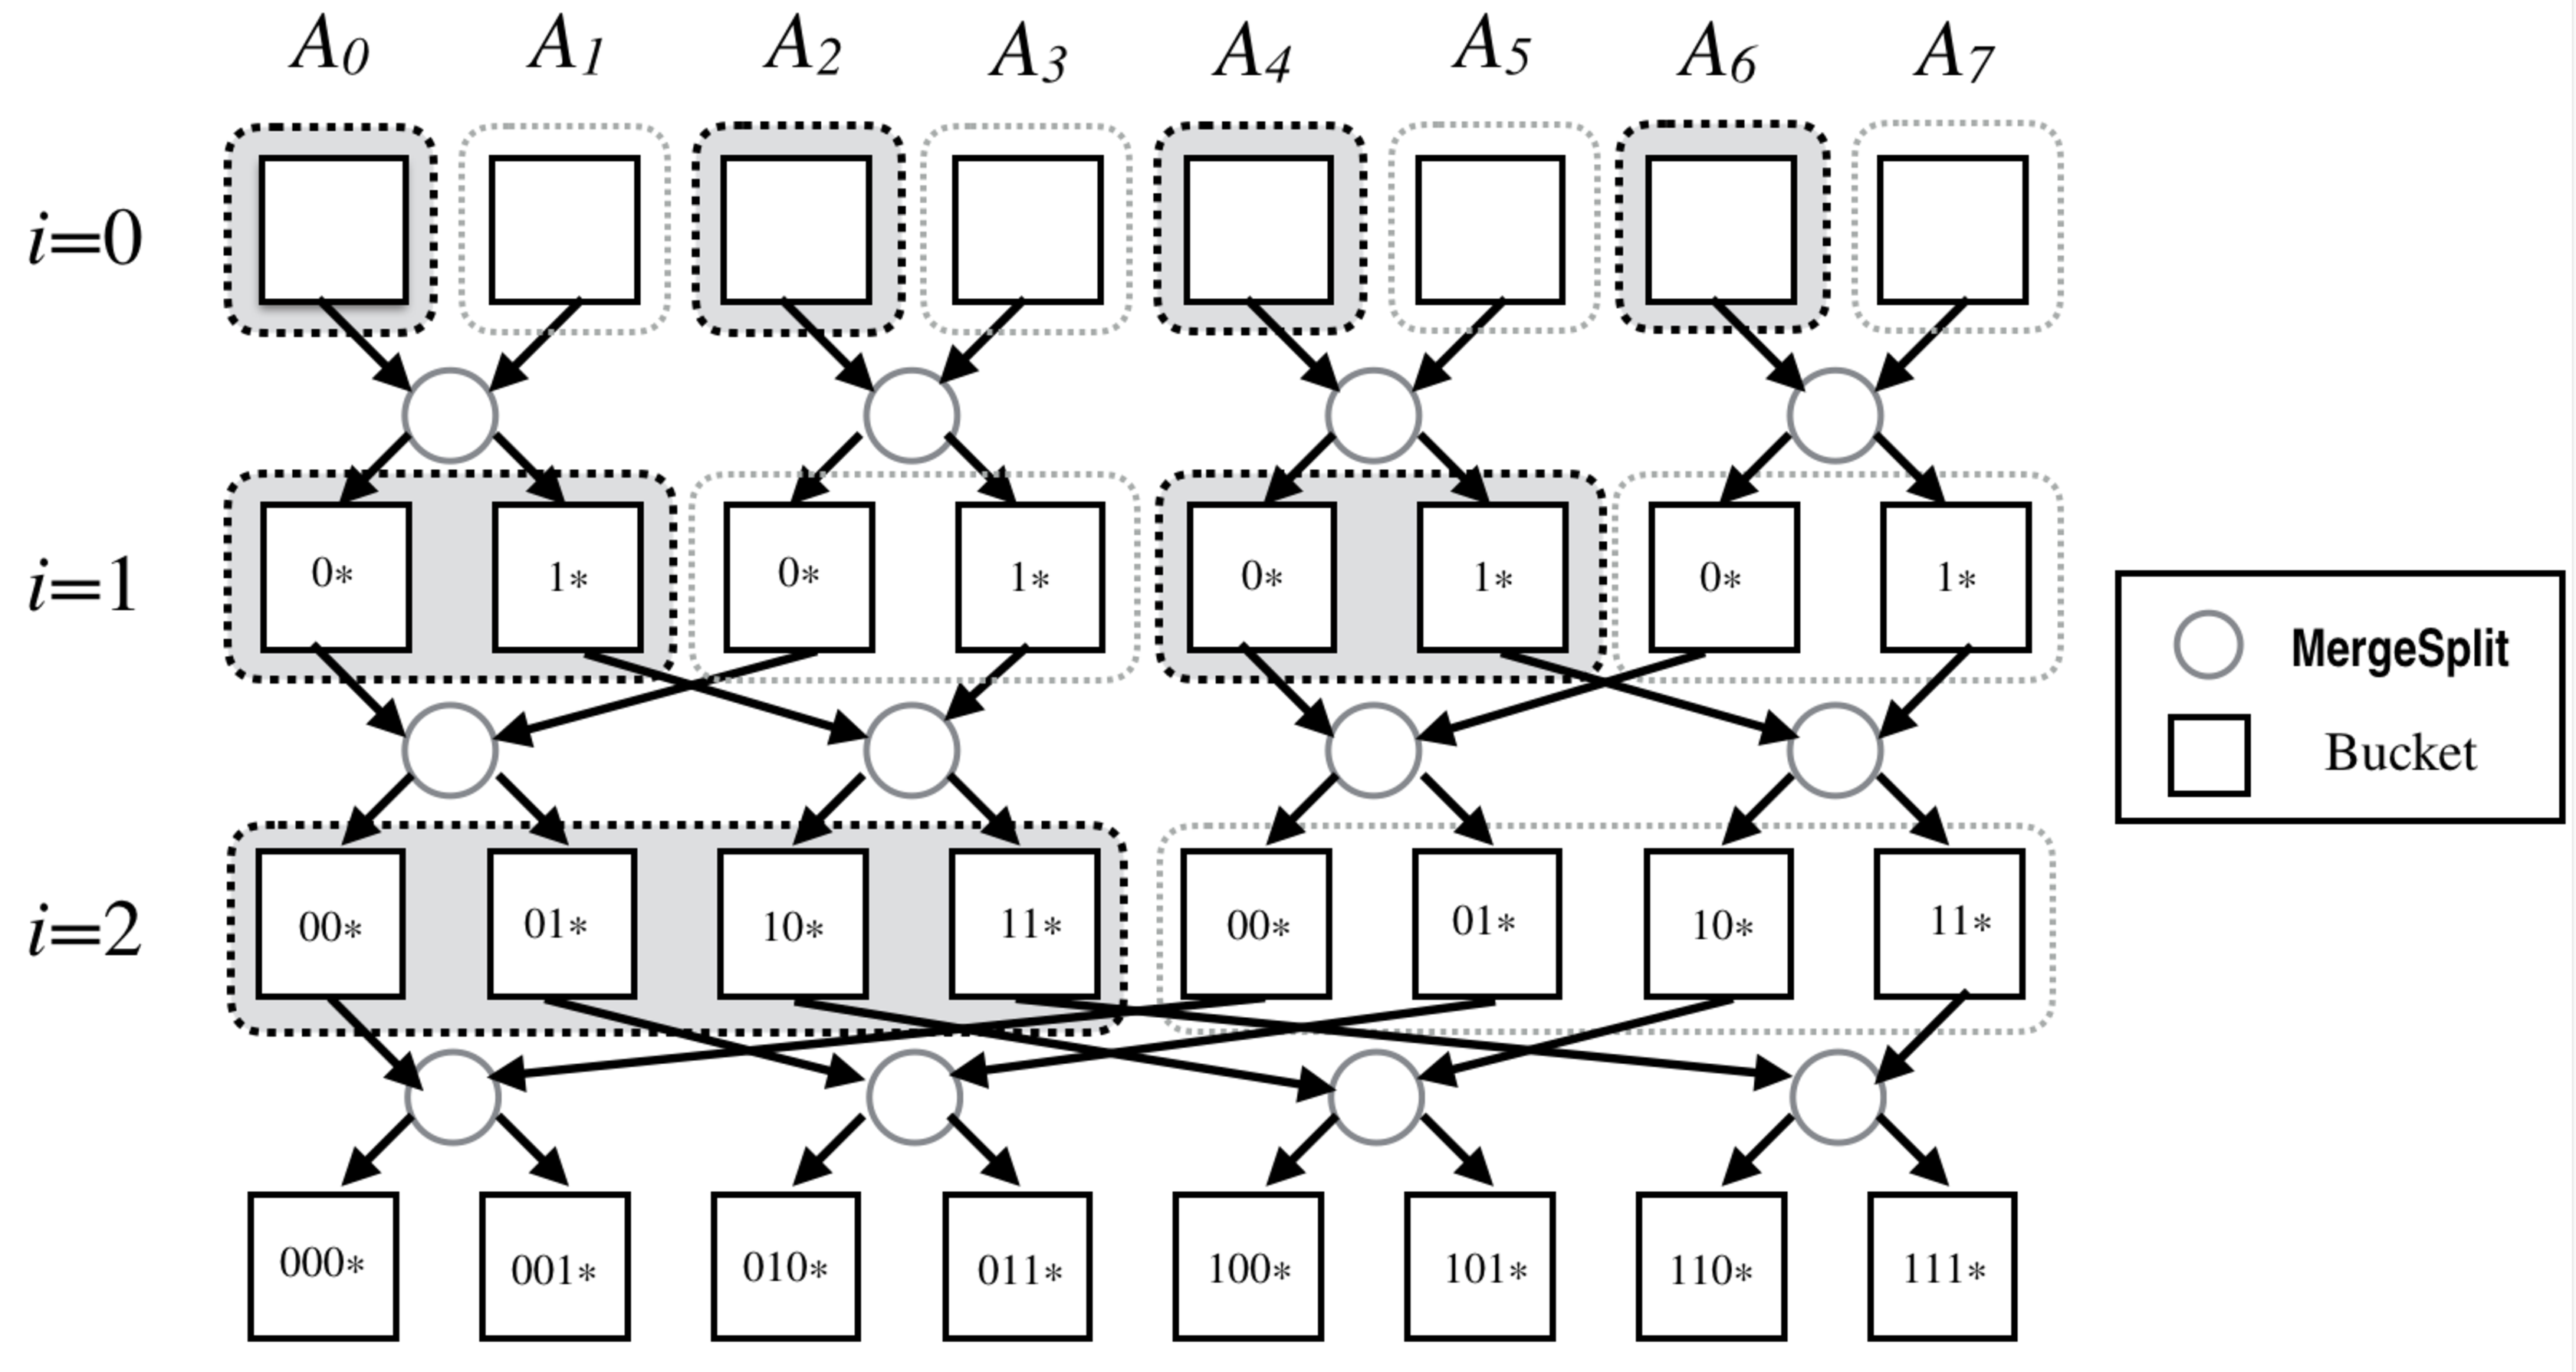
\includegraphics[width=0.7\textwidth]{RadixBucketSort1.pdf}
\captionof{figure}{\textbf{Oblivious random bin assignment with 8 buckets.}
The \textsc{MergeSplit} procedure takes elements from two buckets at level $i$ and put them into two buckets at level $i+1$, according to the $(i+1)$-th most significant bit of the keys. 
At level $i$, every $2^{i}$ consecutive buckets are semi-sorted by the most significant $i$ bits of the keys.}
\label{fig:radix-sort}

%\begin{table*}[t]
\bigskip
\centering
\begin{tabular}{|c|c|c|c|c|}
    \hline
    Algorithm & Oblivious & Client storage & Runtime & Error probability \\
    \hline
    Merge sort & No & $O(1)$ & $2n \log n$ & 0 \\
    Bitonic sort & Yes & $O(1)$ & $n\log^2 n$ & 0 \\
    AKS sort~\cite{aks} & Yes & $O(1)$ & $5.4\times10^7 \times n\log n$ & 0 \\
    Zig-zag sort~\cite{zigzag} & Yes & $O(1)$ & $8\times10^4 \times n\log n$ & 0 \\
    Randomized Shellsort~\cite{RandShellsort} & Yes & $O(1)$ & $24n\log n$ & $\approx n^{-3}$ \\
    \hline
    \textbf{Bucket oblivious sort} & Yes & $2Z$ & $6 n\log n$ & $\approx e^{-Z/6}$\\
    \textbf{Bucket oblivious sort} & Yes & $O(1)$ & $\approx 2n\log n \log^2 Z$ & $\approx e^{-Z/6}$ \\
    \hline   
\end{tabular}
\captionof{table}{\textbf{Runtime of bucket oblivious sort and
classic non-oblivious and oblivious sort algorithms.} Bitonic
sort requires $\frac 14 n \log^2 n$ comparisons. The number of comparisons for AKS
sort and zig-zag sort are cited from \cite{zigzag}. Runtime
represents the number of memory accesses, which is four times the
number of comparisons.}
\label{tab:compare}
%\end{table*}

\end{figure*}

The core of our algorithms is to assign each element to a random bin and then route the elements through a butterfly network to their assigned random bins. 
This part is inspired by Bucket ORAM~\cite{fletcher2015bucket}. 
In more detail, we divide the $n$ elements into $B=2n/Z$ buckets of size $Z/2$ each and add $Z/2$ dummy elements to each bucket.
Now, imagine that these $B$ buckets form the inputs of a butterfly network --- for simplicity, assume $B$ is a power of two.
Each element is uniformly randomly assigned to one of the $B$ output buckets, represented by a key of $\log B$ bits.
The elements are then routed through the butterfly network to their respective destinations.
Assuming the client can store two buckets locally at a time, at level $i$, the client simply reads elements from two buckets that are distance $2^i$ away in level $i$ and writes them to two adjacent buckets in level $i+1$, using the $i$-th bit of each element's key to make the routing decision. 
We refer readers to Figure~\ref{fig:radix-sort} for a graphical illustration.

The above algorithm is clearly oblivious, as the order in which the client reads and writes the buckets is fixed and independent of the input array. If no bucket overflows, all elements reach their assigned destinations. By setting $Z$ appropriately, we can bound the overflow probability.

Our bucket oblivious sort and bucket ORP algorithms are derived from
the above oblivious random bin assignment building block. 

\paragraph{From oblivious random bin assignment to ORP and oblivious sort.}
To obtain a random permutation, we simply remove all dummy elements and randomly permute 
each bucket of the final layer.
Since the client can hold $Z$ elements, permuting each bucket can be done locally. 
We show that the algorithm is oblivious and gives a random permutation despite revealing the number of dummy elements in each destination bucket.
To get oblivious sort, we can first perform ORP on the input array then apply any \emph{non-oblivious, comparison-based} sorting algorithm (e.g., quick sort or
merge sort). We show that the composition of ORP and non-oblivious sort results in an oblivious sort. 

\paragraph{Dealing with small client storage.}
In Section~\ref{sec:O1client}, we extend our algorithms to support $O(1)$ client storage. 
We can rely on bitonic sort to realize the \textsc{MergeSplit} operation that operates on 4 buckets at a time,
which would result in $O(n\log n\cdot \log^2 Z)$ runtime. 

\paragraph{Locality.} Algorithmic performance when the data is stored on disk has been studied in the external disk model (e.g.,~\cite{RuemmlerW94,ArgeFGV97,Vitter01,Vitter06}) and references within). Recently, Asharov et al.~\cite{AsharovCNPRS19} extended this study to oblivious algorithms.  We discuss how our algorithms can be made locality-friendly in Section~\ref{sec:locality}. 


%\paragraph{Organization.}
%The rest of the paper is organized as follows. Our algorithms are simple and intuitive. The access pattern of all our algorithms is deterministic, and therefore security is trivial and all we have to prove is correctness. In Section~\ref{sec:construction} we give our construction and in Section~\ref{sec:extensions} we describe simple extensions. In Appendix~\ref{sec:defs}  define the RAM model of computation and obliviousness. In Appendix~\ref{appx:formal} we give all omitted proofs. 

%
%
%\paragraph{From oblivious bin assignment to ORP.}
%To obtain a random permutation, a simple approach is to remove the dummy elements and permute within each bucket of the final layer. Since the client can hold $Z$ elements, permuting each bucket obliviously can be done locally. 
%
%
%Our bucket oblivious sort and bucket ORP build on top of the above oblivious random bin assignment. 
%To get ORP, simply remove all dummy elements, randomly permute each bucket of the final level, and concatenate the bins.
%To sort, we can simply apply any non-oblivious comparison-based sort (e.g., merge sort) on the randomly permuted elements. 
%
%In Section~\ref{sec:O1client}, we will discuss how to extend our algorithms to support constant client storage
%We can rely on Bitonic sort to realize the ${\bf MergeSplit}$ operation, which would result in $\approx 2n\log n \log^2 Z$ runtime.
%Recently, Asharov et al.~\cite{AsharovCNPRS19} initiate the study of data locality on oblivious algorithms. 
%We observe that our algorithms are be made locality-friendly, and refer readers to Appendix~\ref{sec:locality} for the exact definitions and complexity measures.

%%% Local Variables:
%%% mode: latex
%%% TeX-master: "main"
%%% End:

%!TEX root = main.tex

\newcommand{\memsize}{{N}}
\newcommand{\blocksize}{{b}}
%\newcommand{\negl}{{\sf negl}}
\newcommand{\Y}{{\bf Y}}

%\section*{Appendix}
%In the following we formally define the RAM model of computation, and formally prove obliviousness of our algorithms. 
%
\section{Preliminaries}
\label{sec:defs}

\paragraph{Notations and conventions.}
Let $[n]$ denote the set $\{1,\ldots,n\}$. Throughout this paper, we will use
$n$ to denote the size of the instance and use $\lambda$ to denote the security parameter. 
%A function $\negl$ is called \emph{negligible} if for any constant $c > 0$ and all sufficiently large $\sec$'s, it holds that $\negl < \sec^{-c}$. 
For an ensemble of distributions $\{D_\sec\}$ (parametrized with $\sec$),
we denote by $x \leftarrow D_\sec$ a sampling of an instance from the distribution $D_\sec$. 
We say two ensembles of distributions $\{X_\sec\}$~and~$\{Y_\sec\}$ 
are $\e(\sec)$-statistically-indistinguishable, denoted $\{X_\sec\} \overset{\e(\sec)}{\equiv} \{Y_\sec\}$, 
if for any unbounded adversary $\A$, 
\[
\left|\Pr_{x\leftarrow X_\sec}\left[\A(1^\lambda, x)=1\right] - \Pr_{y\leftarrow Y_\sec}\left[\A(1^\lambda, y)=1\right] \right| \leq \e(\sec) \ .
\]


%For simplicity, we will omit writing the unary security parameter input $1^\lambda$ to all procedures.
%\rl{We are writing the unary security parameter at a lot of places now. Should we add it everywhere and remove this statement?}
% Also, \emph{work} (or bandwidth) is always specified in terms of number of blocks of size $\Omega(\log N)$ accessed.

%\subsection{Memory with Multiple Disks and Data Locality}
%\label{sec:modeling-locality-formal}
%%\paragraph{Random-access machines.}
%%A RAM is an interactive Turing machine that consists of a memory and a CPU.  The
%%memory is denoted as $\mem[N,\bsize]$, and is indexed by the logical
%%address space $[N] = \{1,2,\ldots,N\}$. We refer to each memory word also as a
%%\emph{block} and we use $\bsize$ to denote the bit-length of each block. The CPU
%%has an internal state that consists of $O(1)$ words. The memory supports read/write
%%instructions $(\op,\addr, \data)$, where $\op \in \{\Read,\Write\}$, $\addr \in
%%[N]$ and $\data \in \bit^\bsize \cup \{\bot\}$.  If $\op = \Read$, then
%%$\data=\bot$ and the returned value is the content of the block located in
%%logical address $\addr$ in the memory. If $\op=\Write$, then the memory data in
%%logical address $\addr$ is updated to $\data$.
%%
%%
%%\paragraph{Locality.}
%%We model locality by dividing the memory address space $[N]$ to $\disks$ disks, simply by dividing the memory space to $\disks$ 
%
%
%% \kartik{define bandwidth?}
%To understand the notion of data locality, it may be convenient
%to view the memory as $\disks$ rotational hard drives or other
%storage mediums where sequential accesses are faster than random
%accesses. The program interacting with the memory has to specify
%which disk to access.  
%Each disk is equipped with one read/write head. In order to serve
%a $\Read$ or $\Write$ request with address $\addr$ in some disk
%$\disk \in [\disks]$, the memory has to move the read/write head
%of the disk $\disk$ to the physical location $\addr$ to perform
%the operation.  
%Any such movement of the head introduces cost and delays,  
%and the machine that interacts with the memory would like to
%minimize the  number of move head operations. 
%Traditionally, the latter can be improved by 
%ensuring that the program accesses contiguous regions of the
%memory. 
%% storing related
%% items to physically proximate areas on the memory.  
%However, this poses a great challenge for oblivious computation
%in which data is often continuously shuffled across memory.  
%
%More formally, a memory is denoted as $\mem[N,\bsize,\disks]$,
%consisting of $\disks$ disks, indexed by the address space $[N] =
%\{1,2,\ldots,N\}$, where $\disks \cdot N$ is the size of the
%logical memory. We refer to each memory word also as a
%\emph{block} and we use $\bsize$ to denote the bit-length of each
%block.  
%The memory supports the following two types of instructions.
%\begin{MyItemize}
%\item {\bf \boldmath Move head operation} $(\move,\disk,\addr)$
%moves the head of the $\disk$-th disk ($\disk \in [\disks]$) to point to address $\addr$ within that disk. 
%
%\item {\bf \boldmath A read/write operation} $(\op,\disk,\data)$, 
%where $\op \in \{\Read,\Write\}$, $\disk \in [\disks]$ and $\data \in \bit^\bsize \cup \{\bot\}$. 
%If $\op = \Read$, then $\data=\bot$ and $\mem$ should return the content of the block pointed to by the $\disk$-th disk; 
%If $\op=\Write$, the block pointed to by the $\disk$-th disk is updated to $\data$. The $\disk$-th head is then incremented to point to the next consecutive address, and wrapped around when the end of the disk is reached. 
%
%\end{MyItemize}
%
%\medskip
%\noindent
%{\bf Locality.}
%%\paragraph{Locality.}
%% The number of $\move$ operations defines locality.
%A sequence of memory operations has $(\disks,
%\locparam)$-locality if it contains $\locparam$ $\move$
%operations to a memory that is equipped with $\disks$ disks.  
%
%
%\medskip
%\noindent
%{\bf Relation to the standard memory definition.}
%%\paragraph{Relation to the standard memory definition.} 
%Instead of specifying which disk to read from/write to, we can define a memory of range $[\disks\cdot N] = \{1,\ldots,\disks\cdot N\}$. 
%The address space determines the disk index, and therefore also
%whether or not to move the read/write head. Thus, one can
%consider the regular notion of a RAM program, and our definition
%provides a way to measure the locality of the program. Different implementations
%of the same  functionality can have different locality, similarly to other metrics.

\paragraph{Random-access machines.}
A RAM is an interactive Turing machine that consists of a memory and a CPU.  The
memory is denoted as $\mem[\memsize,\blocksize]$, and is indexed by the logical
address space $[N] = \{1,2,\ldots,N\}$. We refer to each memory word also as a
\emph{block} and we use $\bsize$ to denote the bit-length of each block. The memory supports read/write
instructions $(\op,\addr, \data)$, where $\op \in \{\Read,\Write\}$, $\addr \in
[N]$ and $\data \in \bit^\bsize \cup \{\bot\}$.  If $\op = \Read$, then
$\data=\bot$ and the returned value is the content of the block located in
logical address $\addr$ in the memory. If $\op=\Write$, then the memory data in
logical address $\addr$ is updated to $\data$.
We use standard setting that $\blocksize = \Theta(\log N)$ (so a word can 
store an address).
%We follow the convention that the CPU performs one \emph{word-level operation} per unit time,
%i.e., arithmetic operations (addition or subtraction), 
%bitwise operations (AND, OR, NOT, or shift), memory accesses (read or write), or
%evaluating a pseudorandom function~\cite{oram00,oram09,oram03,oblivhash,LarsenN18,panorama}.

\medskip
\noindent
{\bf Obliviousness.}
Intuitively, a RAM program $M$ obliviously simulates a RAM program $f$ if: (1) it has the same input/output behavior as $f$; (2) There exists a simulator $\Sim(\abs{x})$ that produces access pattern that is statistically close to the access pattern of $M(x)$, i.e., it can simulate all memory addresses accessed by $M$ during the execution on $x$, without knowing $x$. In case the access pattern and the functionality are randomized, we have to consider the joint distribution of the simulator and the output of the RAM program or the functionality. 

%In our sorting algorithm, the access pattern is randomized but the functionality is deterministic. In the oblivious random permutation algorithm, the access pattern is deterministic but the functionality is randomized. As always either the access pattern or the functionality is deterministic, we can consider a simpler definition of obliviousness in which the functionality and the simulation are considered separately. 

For a  RAM machine $M$ and input $x$, let ${\sf AccPtrn}(M(x))$ denote the distribution of memory addresses a machine $M$ produces on an input $x$.
\begin{definition}
A RAM algorithm $M$ obliviously implements the functionality $f$ with $\e$-obliviousness if the following hold:
\begin{eqnarray*}
\left\{\Sim(1^\lambda),f(x)\right\}_{x \in \bit^\lambda} \overset{\epsilon(\lambda)}{\equiv} \left\{ {\sf AccPtrn}(M(x)),M(x)\right\}_{x \in \bit^\lambda}
\end{eqnarray*}
If $\epsilon(\cdot)=0$, we say $M$ is perfectly oblivious. 
%\[ \left\{\Sim(1^\lambda),f(x)\right\}_{x \in \bit^\lambda} 
%\overset{\epsilon(\lambda)}{\equiv} \left\{ {\sf AccPtrn}(M(x)),M(x)\right\}_{x \in \bit^\lambda} \]
\end{definition}

%$$
%$$
%\begin{MyItemize}
%
%\item {\bf $\delta$-Correctness:} For every input $x$ it holds that 
%$$
%\Pr\left[M(x) = f(x) \right] \geq 1- \delta(\abs{x})
%$$
%
%\item {\bf $\e$-Obliviousness:} There exists a simulator $\Sim(\abs{x})$ such that
%$$
%\left\{{\sf AccPtrn}(M(x))\right\}_{\abs{x}} \overset{\e(\abs{x})}{\equiv} 
%\left\{\Sim(\abs{x})\right\}_{\abs{x}}
%$$
%%that produces access pattern that is statistically close to the access pattern of $M(x)$.
%\end{MyItemize}
%\end{definition}

%A functionality $f$ is a (possibly randomized) RAM machine that gets some input $x$ and computes an output $y$. A RAM algorithm $M$ obliviously implements the functionality $f$ if: (1) it has the same input/output behavior as $f$; (2) There exists a simulator $\Sim(\abs{x})$ that produces access pattern that is statistically close to the access pattern of $M(x)$. I.e., it can simulates all memory addresses accessed by $M$ during the execution on $x$, without knowing $x$. Note that all our algorithms have deterministic access pattern, and therefore 
%
%In case where the functionality $f$ is randomized, we require that the joint distribution of the output of the functionality and the output of the simulator would be statistically close to the output of the algorithm $M$ and its access pattern. Formally, we let ${\sf AccPtrn}(M(x))$ denote the distribution of memory addresses a machine $M$ produces on an input $x$. We have:
%
%\begin{definition}[Oblivious machines]
%\label{defn:omachine}
%Let $f,M:\bit^* \rightarrow \bit^*$ be (possibly randomized) RAM programs. We say that $M$ {\em obliviously simulates $f$} if there exists a  simulator $\Sim$ and a negligible function $\epsilon(\cdot)$ such that  for any $\lambda$:% and any input $x$ of size $\lambda$ it holds that:
%\begin{eqnarray*}
%\hspace{-5ex}\lefteqn{\left\{\Sim(1^\lambda),f(x)\right\}_{x \in \bit^\lambda}} \\
%&&\hspace{+5ex}\overset{\epsilon(\lambda)}{\equiv} \left\{ {\sf AccPtrn}(M(x)),M(x)\right\}_{x \in \bit^\lambda}
%\end{eqnarray*}
%If $\epsilon(\cdot)=0$, we say $M$ is perfectly oblivious. 
%\end{definition}

The two main functionalities that we focus on in this paper are the following:

\paragraph{Oblivious sort:}
This is a deterministic functionality in which the input is an array $A[1,\ldots,n]$ of memory blocks (i.e., each $A[i] \in \bit^\blocksize$, representing a key). The goal is to output an array $A'[1,\ldots,n]$ which is some permutation $\pi:[n] \rightarrow [n]$ of the array $A$, i.e., $A'[i] = A[\pi(i)]$, such that $A'[1]\leq \ldots \leq A'[n]$. %Obliviousness is defined using Definition~\ref{defn:omachine}. We denote this functionality as ${\cal F}_{\rm sort}$. 

\paragraph{Oblivious permutation:} 
This is a randomized functionality in which the input is an array $A[1,\ldots,n]$ of memory blocks. The functionality chooses a random permutation $\pi:[n] \rightarrow [n]$ and outputs an array $A'[1,\ldots,n]$ such that $A'[i] = A[\pi(i)]$ for every $i$. %Obliviousness is defined using %Definition~\ref{defn:omachine}. Note that the definition requires that the access pattern does not leak the permutation chosen by the functionality. We denote this functionality ${\cal F}_{\rm perm}$. 
%\end{MyItemize}


%\section{Obliviousness}
%\label{appx:formal}
%In this section we provide proofs for obliviousness of our constructions. In Section~\ref{sec:rand:functionality} we formally define the ideal functionality of the random bin assignment (Algorithm~\ref{code:obin}). 
%
%
%\subsection{\boldmath Random Bin Assignment: Functionality}
%\label{sec:rand:functionality}
%We start with defining the oblivious random bin assignment functionality, which we denote by $f_{\rm randbin}$. In a nutshell, given some input array ${\bf X}$ we consider an output array which has twice the size of the input array, and we consider the output array as $B$ consecutive bins. We assign each ``real'' element of the input array into a random bin in the output array, and pad each bin with dummy elements. We will show how to realize the functionality for $Z := \alpha \log \lambda$ with $\alpha \in \omega(1)$ and $\lambda$ is the security parameter. 
%
%
%\begin{myfunc}
%[\boldmath ${\cal F}_{\rm randbin}(\X,Z)$]
%\label{func:bin-assignment}
%The random bin assignment functionality ${\cal F}_{\rm randbin}(\X,Z)$ is defined as follows:
%\begin{MyItemize}
%\item {\bf Input:} an input an array $\X$ of length $n$ containing real and dummy elements, and a bin size~$Z$. 
%\item {\bf The functionality:} 
%\begin{MyEnumerate}
%\item Define an output array $\Y$ of size $2n$, containing $B = 2n/Z$ bins of size $Z$ each, denoted as $\Y_1,\ldots,\Y_B$. 
%\item For every real element in $\X$ choose a random destination bin $i \gets [B]$, and place the element in the $i$th output bin. 
%\item If some output bin contains more than $Z$ elements, then {\sf abort}. 
%\item Pad each output bin to its maximal capacity using dummy elements. Order each output bin as follows: 
%(1) all real elements appear before dummies;
%and (2) real elements are ordered according to their ordering (indices) in the input array $\X$.
%\end{MyEnumerate}
%\end{MyItemize}
%\end{myfunc}
%
%
%\begin{lemma}
%Let $Z = \alpha \log \lambda$ for any super-constant function $\alpha(\lambda)$.
%Algorithm~\ref{code:obin}
%obliviously simulates ${\cal F}_{\rm randbin}$ (i.e., Functionality~\ref{func:bin-assignment}) with $\epsilon(n, Z) = 2n/Z \cdot \log(2n/Z) \cdot e^{-Z/6}$ failure probability. %The algorithm completes in $O(\frac{n}{Z}\log n \cdot T_{\sf MergeSplit}(Z))$ work, where $T_{\sf MergeSplit}(Z)$ .
%\label{lem:randbin}
%\end{lemma}
%\begin{proof}
%The access pattern of Algorithm~\ref{code:obin} is deterministic and is independent of the input, and therefore it can be simulated easily. Moreover, since it is deterministic, it suffices to consider correctness and access pattern separately, and there is no need to consider the joint distribution. 
%As for correctness, we claim that the algorithm implements Functionality~\ref{func:bin-assignment}. Specifically, the functionality and the algorithm choose the same bin assignment for all elements with the exact same probability. Moreover, for the same bin assignments for all elements, the functionality and the algorithm result in the same output, except for a negligible probability of failure. This occurs when there is some internal overflow in the algorithm in one of the iterations $i \in \{1,\ldots,\log B\}$, which does not occur in the functionality. 
%%As for efficiency, we run ${\sf MergeSplit}$ exactly $B \log B$ times, which results in $O(\frac{n}{Z}\log n \cdot T_{\sf MergeSplit}(Z))$. 
%%	%Sorting each bin results in $B \cdot (Z \log^2 Z) = n \log^2 Z$, which is smaller than $O(n \log n)$. 
%\end{proof}
%%
%%\subsection{Oblivious Sort from Oblivious Random Bin Assignment}
%%\label{sec:obliviousSortFromRandomBinAssignment}
%%
%%We formalize the composition theorem: Given an oblivious random bin assignment, 
%%%\paragraph{Oblivious sort from random bin assignment algorithm  and non-oblivious sort.}
%%Given a random bin assignment algorithm 
%%${\sf ObliviousRandomBin}$ and a non-oblivious
%%comparison-based sorting algorithm ${\sf NonObliviousSort}$ (e.g., Merge-Sort), one can 
%%easily construct
%%an oblivious sorting algorithm as follows. 
%%%
%%\begin{myalgorithm}
%%[${\sf ObliviousSortFromRandomBinAssignment}(\X)$]
%%\label{alg:sort-from-random-bin}
%%\leavevmode
%%\begin{MyEnumerate}%[leftmargin=5mm]
%%\item 
%%Given an input array $\X$, invoke the random bin assignment algorithm to receive $\Y: = {\sf ObliviousRandomBin}(\X)$. Note that in each ``bin'' of $\Y$, the real elements appear before the dummy elements, and are sorted. Moreover, $\abs{\Y}=2\abs{\X}$.  
%%
%%%\item Obliviously sort each bucket $A_0,\ldots,A_{B-1}$ using Bitonic Sort, sorting the real elements according to their keys, and preferring real elements over dummy elements. 
%%
%%
%%\item Sort $\Y$ using a (non-oblivious) comparison-based sorting algorithm. 
%%That is, invoke ${\Y'} := {\sf NonObliviousSort}(\Y)$, while preferring real elements over dummy elements. 
%%Formally speaking, a sorting algorithm is comparison-based if the physical access pattern depends only on the relative ranking of elements in the input. 
%%A technical condition we need is that no two elements have the same rank. This can be ensured by resolving any tie consistently by the initial location of the elements in the array $\Y$.
%%
%%\item Now, all dummy elements appear at the $n$ last locations of $\Y'$. Truncate the last $n$ elements of $\Y'$. 
%%
%%\end{MyEnumerate}
%%\end{myalgorithm}
%%
%%%Let ${\sf Truncate}$ denote the last step of the above algorithm. Then, our sorting algorithm can be described as the following simple composition 
%%%$$ {\sf Truncate}({\sf NonObliviousSort}({\sf ObliviousRandomBin}(\X))) \ .$$
%%
%%\paragraph{Why is it oblivious?} 
%%Given that we do not fully permute the input array, a natural question is why the above composition is still oblivious. Essentially, the composition still holds since there is a 1-to-1 mapping between any input of the array and every possible output of the ${\cal F}_{\rm randbin}$ functionality, i.e., every possible input of the non-oblivious sorting algorithm. This mapping is exactly the random assignment of the destination bins. Therefore,  every access pattern in the non-oblivious sorting part of the algorithm, can be justified with some specific random assignment on the input array, for every possible ordering of the input array. However, some of the  assignments are ``invalid'' due to overflows; yet, overflows occur with negligible probability, and therefore we get statistical security. We proceed to the formal proof of security:
%%
%%\begin{lemma}[From oblivious random bin to oblivious sort]
%%Suppose that {\sf ObliviousRandomBin} is a statistically (or perfectly resp.)
%%oblivious random bin assignment algorithm.
%%Then, 
%%the above algorithm is a statistically (or perfectly resp.) secure 
%%oblivious sorting algorithm. 
%%\label{lem:orpsort}
%%\end{lemma}
%%\begin{proof}
%%Since the functionality is deterministic, we can consider obliviousness and correctness separately. Correctness of the algorithm is trivial. 
%%We next prove the obliviousness of the algorithm. 
%%We prove for the case of perfect security, since statistical security is similar,
%%except that we replace ``identically distributed'' with ``statistically close''.
%%
%%
%%Let ${\sf SimRandBin}$ be the simulator algorithm for 
%%the underlying oblivious random bin assignment.
%%Consider any given input $\X$ of length $n$, 
%%and let $(\Y, {\sf addressesRandBin})$ 
%%denote the joint distribution of the outcome array $\Y$ and the addresses
%%accessed during an execution of the oblivious random bin assignment.
%%Lemma~\ref{lem:randbin} implies that:
%%$$
%%\left(\Y, {\sf addressesRandBin}\right) \equiv \left({f}_{\rm randbin}(\X), {\sf SimRandBin}(1^n,|\X|)\right)  \ . \vspace{-1ex}
%%$$
%%Let ${\sf SortAddresses}(\Y)$ 
%%denote the addresses observed during an execution 
%%of the truncation algorithm and the non-oblivious, comparison-based 
%%sorting algorithm upon receiving input array $\Y$.
%%We thus have that\vspace{-1ex}
%%\begin{eqnarray*}
%%\hspace{-15ex}\lefteqn{\left({\sf SortAddresses}(\Y), {\sf addressesRandBin}\right)}\\
%%&& \hspace{+15ex}\equiv 
%%\left({\sf SortAddresses}({f}_{\rm randbin}(\X)), {\sf SimRandBin}(1^n,|\X|)\right) \ .   \vspace{-1ex}
%%\end{eqnarray*}
%%For any comparison-based 
%%sort, its access patterns depend only on 
%%the relative ranking of the input elements. Since without loss of generality, 
%%we assumed that the input array $\X$ always has distinct values, and we carefully defined how to avoid any ties, 
%%we have that\vspace{-1ex}
%%$$
%%{\sf SortAddresses}({f}_{\rm randbin}(\X)) \equiv
%%{\sf SortAddresses}({f}_{\rm randbin}([|\X|])) \ , \vspace{-1ex}
%%$$
%%where $[|\X|] = \{1,\ldots,|\X|\}$. 
%%Now, 
%%observe that we can construct a simulator 
%%${\sf SimObliviousSort}$
%%that simply outputs 
%%$$
%%{\sf SortAddresses}({f}_{\rm randbin}([|\X|])), {\sf SimRandBin}(1^n,|\X|)
%%$$
%%This simulator's output is identically distributed
%%as the real-world access patterns of executing
%%the aforementioned sorting algorithm, i.e., to $({\sf SortAddresses}(\Y), \allowbreak{\sf addressesRandBin})$. 
%%\end{proof}
%%
%%%We therefore conclude:
%%%\begin{corollary}
%%%\label{cor:rand-bin-using-bitonic}
%%%Let $Z = \alpha \log \lambda$ for any super-constant function $\alpha(\lambda)$, and assume that a client can store $4\cdot Z$ elements locally. 
%%%Algorithm~\ref{alg:bucket-sort}, where ${\sf MergeSplit}$ 
%%%obliviously simulates ${\cal F}_{\rm randbin}$ (i.e., Functionality~\ref{func:bin-assignment}) with $\negl$ statistical 
%%%failure. The algorithm completes in $O(n \log n)$ work.
%%%\end{corollary}
%%
%%%\medskip
%%%\noindent
%%%{\bf Building blocks.} Moreover, in Appendix~\ref{sec:building-blocks} we review some building blocks that we will use in our construction, including oblivious sorts, {\sf Dedup} -- an algorithm that removes duplicates obliviously based on oblivious sorts, and Oblivious Bin Packing -- an algorithm that receives an array as an input, where each element is marked with some destination bin, and the algorithm obliviously routes the elements into the bin, while padding each bin to its maximal capacity with dummy elements. This is again implemented using oblivious sorts. See Appendix~\ref{sec:building-blocks} for further details.   
%%
%%%%% Local Variables:
%%%%% mode: latex
%%%%% TeX-master: "main"
%%%%% End:

%!TEX root = main.tex




\section{Our Construction} 
\label{sec:construction}
\label{sec:random-bin-assignment}

We first present the oblivious random bin assignment algorithm (Section~\ref{sec:obin})  and then use it to implement our bucket oblivious random permutation (Section~\ref{sec:ORP}) and bucket oblivious sort (Section~\ref{sec:osort}).

\newcommand{\val}{{\sf value}}
\newcommand{\pref}{{\sf pref}}

\begin{figure*}[h!]
\centering

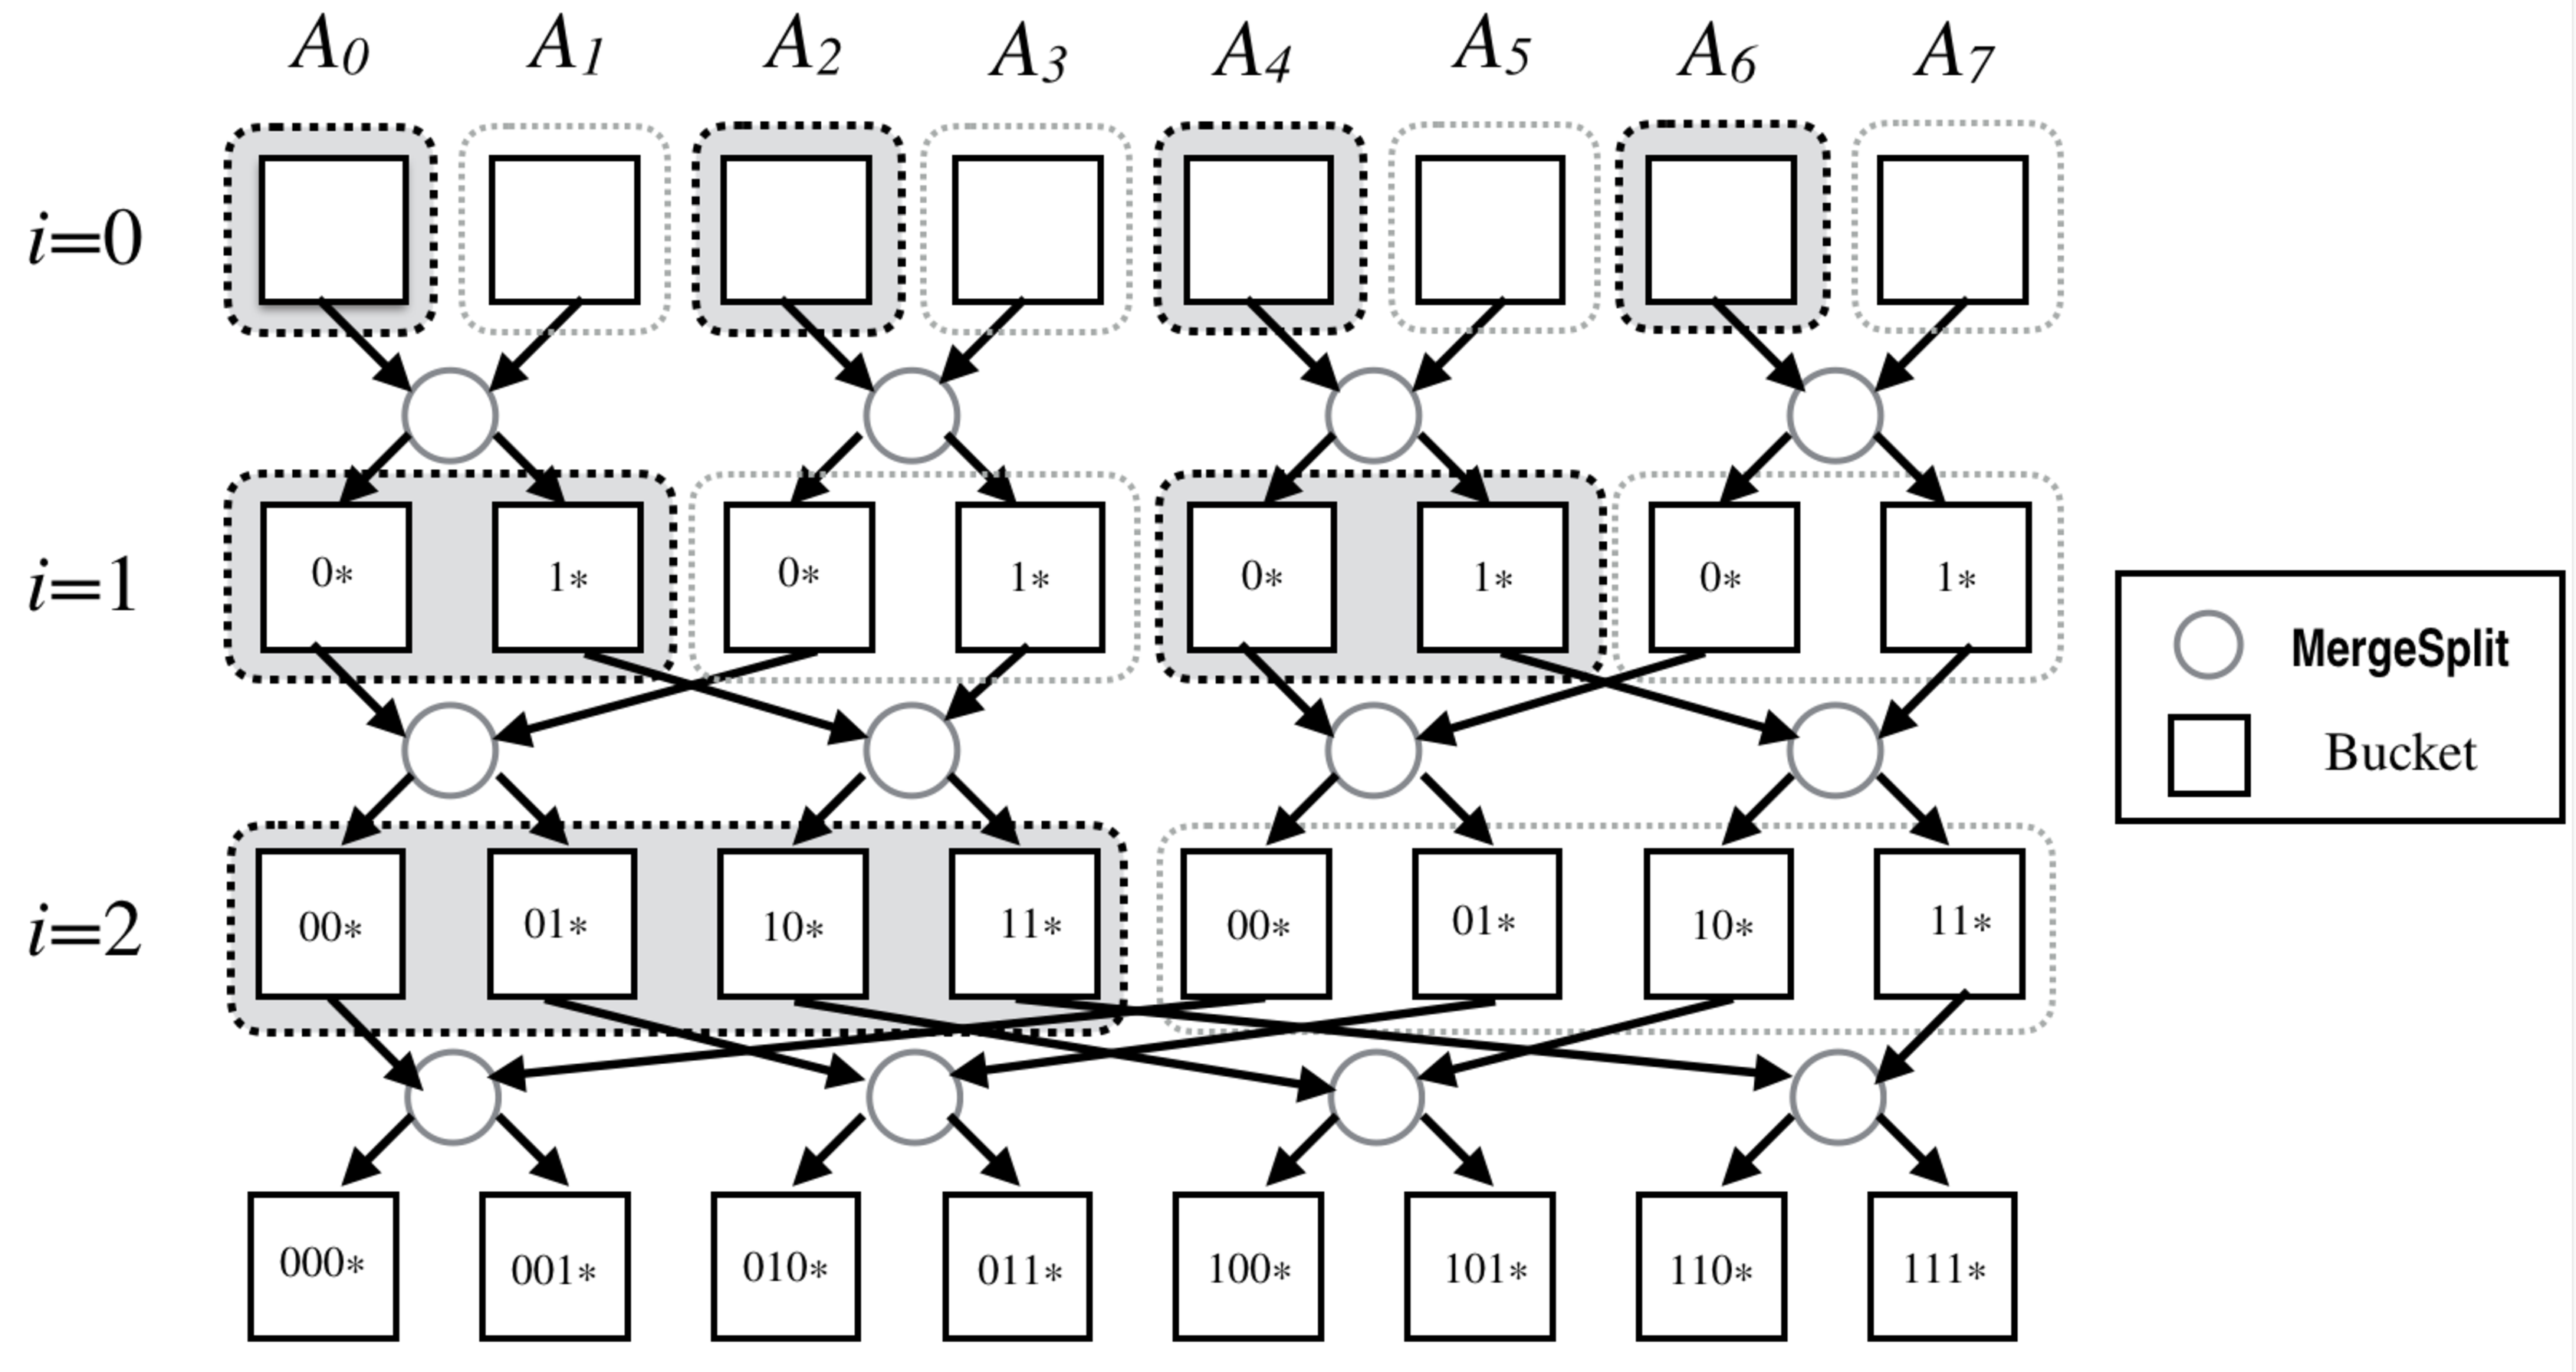
\includegraphics[width=0.75\textwidth]{RadixBucketSort1.pdf}
\captionof{figure}{Oblivious random bin assignment with 8 buckets.}
%The \textsc{MergeSplit} procedure takes elements from two buckets at level $i$ and put them into two buckets at level $i+1$, according to the $(i+1)$-th most significant bit of the keys. 
%At level $i$, every $2^{i}$ consecutive buckets are semi-sorted by the most significant $i$ bits of the keys.
\label{fig:radix-sort}

\bigskip
\begin{algorithm}[Oblivious Random Bin Assignment]
\begin{algorithmic}
\State
\State \textbf{Input}: an array $\X$ of size $n$
\State Choose a bucket size $Z$ and let $B$ be the smallest power of two that is $\geq 2n/Z$. 
\State Define $(\log B+1)$ arrays, each containing $B$ buckets of size $Z$. Denote the $j$-th bucket of the $i$-th array $A_j^{(i)}$.
\State For each element in $\X$, assign a uniformly random key in $[0,B-1]$.
\State Evenly divide $\X$ into $B$ groups. Put the $j$-th group into $A_j^{(0)}$ and pad with dummy elements to have size $Z$.

\For {$i=0,\ldots,\log B-1$}
    \For {$j=0,\ldots,B/2$}
        \State $(A^{(i+1)}_{2j}, A^{(i+1)}_{2j+1}) \leftarrow \textsc{MergeSplit}(A^{(i)}_{j'+j}, A^{(i)}_{j'+j+2^i}, i)$ where $j'=\lfloor j / {2^i} \rfloor \cdot 2^{i+1}$
        \State \Comment{Input: $j$-th pair of buckets with distance $2^i$ in $A^{(i)}$; Output: $j$-th pair of buckets in $A^{(i+1)}$}
        %\State Let $(A_0, A_1$) be the $j$-th pair of buckets with distance $2^i$ in $A^{(i)}$ 
        %\State Let $(A'_0, A'_1)$ be the $j$-th pair of buckets in $A^{(i+1)}$
        %\State $(A'_0, A'_1) \leftarrow \textsc{MergeSplit}(A_0, A_1, i)$ 
        
    \EndFor
\EndFor    
\State \textbf{Output:} $A^{(\log B)}$

\medskip
\Function{$(A'_0, A'_1) \leftarrow$ MergeSplit}{$A_0, A_1, i$}
    \State $A'_0$ receives all real elements in $A_0 \cup A_1$ where the $(i+1)$-st MSB of the key is $0$   
    \State $A'_1$ receives all real elements in $A_0 \cup A_1$ where the $(i+1)$-st MSB of the key is $1$
    \State If either $A'_0$ or $A'_1$ receives more than $Z$ real elements, the procedure aborts with {\sf overflow}
    \State Pad $A'_0$ and $A'_1$ to size $Z$ with dummy elements and return $(A'_0, A'_1)$
\EndFunction   
\end{algorithmic}
\label{code:obin}
\end{algorithm}

\bigskip
%\begin{table*}[t]
\centering
\begin{tabular}{|c|c|c|c|c|}
    \hline
    Algorithm & Oblivious & Client storage & Runtime & Error probability \\
    \hline
    merge sort & no & $O(1)$ & $2n \log n$ & 0 \\
    Bitonic sort & yes & $O(1)$ & $n\log^2 n$ & 0 \\
    AKS sort & yes & $O(1)$ & $5.4\times10^7 \times n\log n$ & 0 \\
    Zigzag sort & yes & $O(1)$ & $8\times10^4 \times n\log n$ & 0 \\
    Randomized Shellsort & yes & $O(1)$ & $24n\log n$ & $\approx n^{-3}$ \\
    \hline
    \textbf{Bucket oblivious sort} & yes & $2Z$ & $6 n\log n$ & $\approx e^{-6/3}$\\
    \textbf{Bucket oblivious sort} & yes & $O(1)$ & $2n\log n \log^2 Z$ & $\approx e^{-6/3}$ \\
    \hline   
\end{tabular}
\captionof{table}{Runtime of bucket oblivious sort and classic non-oblivious and oblivious sort algorithms.}
\label{tab:compare}
%\end{table*}

\end{figure*}
\subsection{Oblivious Random Bin Assignment.}
\label{sec:obin}

The input to the oblivious random bin assignment algorithm is an array $\X$ of $n$ elements. 
The goal is to obliviously and uniformly randomly distribute the elements into a set of bins. Each element is assigned to independent random bin, and elements are then routed into the bins obliviously. 

The algorithm first chooses a bucket size $Z$, which can be set to the security parameter $\sec$. 
Then, it constructs $B=\lceil 2n/Z \rceil$ buckets each of size $Z$.
Without loss of generality, assume $B$ is a power of $2$ --- if not, pad it to the next power of 2. Note that the algorithm introduces $n$ dummy elements, and the output is twice the size of the input array. %If needed, see Appendix~\ref{appx:formal} for a formal definition of the functionality. 

%also assume elements in $\X$ are distinct --- if not, we can use the indices of the elements within $\X$ to break ties.

Figure~\ref{fig:radix-sort} gives a graphic illustration of the algorithm for 8 input buckets and Algorithm~\ref{code:obin} gives the pseudocode.
Each element in $\X$ is assigned a random key in $[0, B-1]$ which represents a destination bucket.
Next, the algorithm repeatedly calls the \textsc{MergeSplit} subroutine to exchange elements between bucket pairs in $\log B$ levels to distribute elements into their destination buckets. 
The operation $(A'_0,A'_1)\leftarrow \textsc{MergeSplit}(A_0,A_1,i)$ involves four buckets at the time, distributing the elements in the two input buckets $A_0$ and $A_1$ into two output buckets $A'_0$ and $A'_1$.
$A'_0$ receives all the keys with $(i+1)$-th most significant bit (MSB) as 0 and $A'_1$ receives all the keys with $(i+1)$-th MSB as 1.


For now, assume the client can locally store two buckets.
For each \textsc{MergeSplit}, it reads (and decrypts) the two input buckets, swaps elements in the two buckets according to the above rule, and writes to the two output buckets (after re-encryption).
It is then easy to see that Algorithm~\ref{code:obin} is oblivious since the order in which the client reads and writes the buckets is fixed and independent of the input array.
%We discuss how to extend the algorithm to work with $O(1)$ client storage in Section~\ref{sec:O1client}. 

When no bucket overflows, all real elements are correctly put into their assigned bins.
We now show that the probability of overflow is exponentially small in $Z$. 
Intuitively, this is because each bucket contains (in expectation) half dummy elements that serve as a form of ``slack'' to disallow overflow.

\begin{lemma}
\label{lemma:shuffle}
Overflow happens with at most $\epsilon(n, Z) = 2n/Z \cdot \log(2n/Z) \cdot e^{-Z/6}$ probability.
\end{lemma}
\begin{proof}
\label{clm:proof-shuffle}
Consider a bucket $A^{(i)}_b$ at level $i$.
%Let $T$ be the set of real elements. For $t \in T$, $i \in \{1,\ldots,\log B\}$ and $b \in [B]$, let $X_{i,b}^{t}$ be the indicator random variable that $t$ is assigned to bucket $A^{(i)}_b$.
%$X_{i,b}=\sum_{t \in T}X_{i,b}^{t}$ denotes the load of $A^{(i)}_b$. 
Observe that this bucket can receive real elements from $2^i$ initial buckets, each containing $Z/2$ real elements.
For each such element, we have chosen an independent and uniformly random key;
the element reaches $A^{(i)}_b$ only when the most significant $i$ bits of its key match $b$,
which happens with exactly $2^{-i}$ probability.
A Chernoff bound shows that $A^{(i)}_b$ overflows with less than $e^{-Z/6}$ probability.
Hence, a union bound over all levels and all buckets 
shows that overflow happens with less than $B \cdot \log B \cdot e^{-Z/6} = \epsilon(n,Z)$ probability.
\end{proof}

%In Appendix~\ref{appx:formal} we formally describe the ideal functionality of oblivious random bin assignment, and show that the above describe algorithm obliviously implements this functionality. 

\subsection{Bucket Oblivious Random Permutation.}
\label{sec:ORP}

After performing the oblivious random bin assignment, ORP can be simply achieved as follows:
scan the array and delete dummy elements from each bin (note that within each bin it is guaranteed that the real elements appear before the dummy elements). Then obliviously permute each bin and finally concatenate all bins.  We have:

%The ORP reveals the loads of the output buckets of bin assignment, that is, the number of real elements in each bucket. 

\begin{lemma}
Bucket ORP oblivious implement the permutation functionality except for $\e(n,Z)$ probability. 
\end{lemma}

\begin{proof}
We first describe the simulator. 
The access pattern of the oblivious bin assignment algorithm is deterministic and the same for every input, where the overflow even is independent of the input itself. Therefore, it is easy to simulate the bin assignment. 
The simulator then pretends to simulate the randomly permuting of each bin. 
Then, 
the simulator chooses random loads $\vec{k}=(k_0, k_1, \ldots, k_{B-1})$, where $k_i$ is the load of the real elements in the $i$th bin. This is done by simply throwing $n$ elements into $B$ bins (``in the head''). If there is some $i$ for which $k_i > Z$ then the simulator aborts. The removal of the dummy elements is equivalent to the revealing of these loads. 

Clearly, $\vec{k}$ are distributed the same as in the real execution. The only difference between the simulated access pattern and the real one is in the case where the algorithm aborts as a result of an overflow before the last level, which occurs with at most $\e(n,Z)$ probability. 

We next show that the output of the algorithm is a random permutation, conditioned of the access pattern. As we previously described, it is actually enough to condition on the vector of random loads $\vec{k}=(k_0, k_1, \ldots, k_{B-1})$. We show that given any such vector, all permutations are possible.  

Fix a particular load $\vec{k}=(k_0, k_1, \ldots, k_{B-1})$. The algorithm works by first assigning the real elements into the bins, and then permuting within each bin. For every input, there are exactly ${n \choose k_0,\ldots,k_{B-1}}$ ways to distribute the real elements into the bins while achieving the vector of loads $\vec{k}$. Then, each bin is individually permuted, i.e., within each bin $i$, we have $k_i$ different possible ordering. Overall, 
the total number of possible outputs with that load is then
\[{n \choose k_0,\ldots,k_{B-1}} \cdot k_0! \cdot \ldots \cdot k_{B-1}! = n!\]
That is, even conditioned on some specific loads $\vec{k}=(k_0, k_1, \ldots, k_{B-1})$, all permutations are still possible.
Therefore, for every $\pi$, $\Pr\left[\Pi = \pi \mid \vec{K}=\vec{k} \right] = \frac 1 {n!}$, and
\[ \Pr\left[\Pi = \pi\right] = \sum_{\vec{k}} \Pr\left[\Pi = \pi \mid \vec{K}=\vec{k} \right] \cdot \Pr\left[\vec{K}=\vec{k}\right] = \frac {1}{n!} \]
%&= \frac {1}{n!} \cdot \sum_{\vec{k}} \Pr\left[\vec{K}=\vec{k}\right] = \frac {1}{n!}

The ORP fails only when some bin overflows during the oblivious random bin assignment, which happens with $\epsilon(n,Z)$ probability.
\end{proof}

\subsection{Bucket Oblivious Sort.}
\label{sec:osort}
Once we have ORP, it is easy to achieve oblivious sort: just invoke any non-oblivious comparison-based sort after ORP.

Since the functionality is deterministic, it is enough to consider separately correctness and simulation. Correctness follows from directly from the correctness of the ORP and the non-oblivious sort. As for obliviousness, given any input array, one can easily simulate the algorithm by first randomly permuting the array and then running the comparison-based non-oblivious sort. 
The access patterns of a comparison-based sort depend only on the relative ranking of the input elements, which is independent of the input array once the array has been randomly permuted. 

\subsection{Efficiency.}
\label{sec:efficiency}

We analyze the efficiency of our algorithms and compare them to classic non-oblivious oblivious sorting algorithms in Table~\ref{tab:compare}.
We measure runtime using the number of memory accesses the clients needs to perform on the server.



% Merge sort, a well known non-oblivious sort, runs in $2n\log n$ time. 
% It has in $\log n$ stages; each stage merges smaller sorted subarrays into larger sorted subarrays,
% which reads and writes the entire array in the process.
% Bitonic sort uses $\frac 14 n\log^2 n$ comparisons.
% According to~\cite{zigzag}, the AKS sorting network has $13613047 n\log n$ comparisons and the Zigzag sort uses $19600n\log n$ comparisons (with best known explicit constructions). 
% Randomized Shellsort~\cite{RandShellsort} needs $6n\log n$ comparisons (there are $\log n$ iterations, six passes per iteration, and $n$ comparisons per pass). 
% The number of memory accesses is four times of the number of
% comparisons for Bitonic, AKS, Zigzag, and randomized Shellsort.


For our algorithms, assuming the client can store $2Z$ elements locally, each $2n$-sized array is read and written once and there are $\log(2n/Z)<\log n$ of them.
So oblivious bin assignment and bucket ORP run in (less than) $4n\log n$ time.
Note that the last step of ORP, i.e., permuting each output bucket, can be incorporated with the last level of oblivious bin assignment.
Bucket oblivious sort additionally invokes a non-oblivious sort, and thus runs in $6n\log n$ time. 
This is within $3\times$ of merge sort and beats bitonic sort when $n$ is moderately large;
for example, $5\times$ faster than bitonic for $n=2^{30}$.
For an overflow probability of $2^{-80}$ and most reasonable values of $n$, $Z = 512$ suffices. 


%%% Local Variables:
%%% mode: latex
%%% TeX-master: "main"
%%% End:

% !TEX root =  main.tex

\section{Extensions}
\label{sec:extensions}

\subsection{Extension to Constant Client Storage.}
\label{sec:O1client}
We now discuss how to extend our algorithms to the case where the client can only store $O(1)$ elements locally.

Each \textsc{MergeSplit} can be realized with a single invocation of Bitonic sort.
Concretely, we first scan the two input buckets to count how many real elements should go to $A'_0$ vs. $A'_1$, then tag the right number of dummy elements to go to either direction, and finally perform the Bitonic sort.

Next, we need to permute each output bucket obliviously with $O(1)$ local storage. 
This can be done as follows. 
First, assign each element in a bucket a uniformly random label of $\Theta(\log n)$ bits. 
Then, obliviously sort the elements by their random labels using Bitonic sort. 
Since the labels are ``short'' (i.e., logarithmic in size), we may have collisions with $n^{-c}$ probability for some constant $c$, in which case we simply retry. 
In expectation, it succeeds in $1+o(1)$ trials. 

%or use the method in Chan et al.~\cite{opramdepth}[Lemma 10] \rl{what is this?}

Since we invoke $B/2$ instances of Bitonic sort on $2Z$ elements at each level,
the runtime is roughly $\log B \cdot B/2 \cdot 2Z \log^2 (2Z)) \approx 2 n\log n \log^2 Z$. 
%In this case, our ORP and oblivious sort run in approximately $160n\log n$ time. \rl{Not competitive. is this part worth it?}

\subsection{Better Asymptotic Performance.}
Our algorithms can also be extended to have better asymptotic performance.
For this instantiation, we use a primitive called oblivious tight compaction.
Oblivious tight compaction receives $n$ elements each marked as either 0 or 1, and outputs a permutation of the $n$ elements such that all elements marked 0 appear before the elements that are marked 1. 
It should not be hard to see that oblivious tight compaction can be used to achieve \textsc{MergeSplit}.
Using the $O(1)$-client-storage and $O(n)$-time oblivious tight compaction construction from~\cite{asharov2018optorama}, bucket oblivious sort achieves $O(n\log n + n\log^2Z)$ runtime and $O(1)$ client storage.
Setting $Z=\omega(1)\log n$, bucket oblivious sort achieves $O(n\log n)$ runtime, $O(1)$ client storage, and a negligible in $n$ error probability.

\subsection{Locality.}
\label{sec:locality}
Algorithmic performance when the data is stored on disk has been studied in the external disk model (e.g.,~\cite{RuemmlerW94,ArgeFGV97,Vitter01,Vitter06}) and references within). Recently, Asharov et al.~\cite{AsharovCNPRS19} extended this study to oblivious algorithms. In this setting, an algorithm 
is said to have $(p, \ell)$ locality if it has access 
to $p$ disks and 
accesses in total $\ell$ discontiguous memory regions in all disks combined. As an example, it is not hard to see that merge sort is non-oblivious sorting algorithm that sorts an array of size $n$ in $O(n \log n)$ and $(3,\log n)$-locality, whereas quick sort  is not local for any reasonable $p$. 
This locality metric is motivated by the fact that real-world storage
media such as disks support sequential accesses
much faster than random seeks. Thus an algorithm that 
makes mostly sequential accesses would execute much faster in practice than one that  
makes mostly random accesses --- even if the two have the same runtime in a standard
word-RAM model. 

Guided by this new metric, Asharov et al.~\cite{AsharovCNPRS19} consider how to design oblivious algorithms and ORAM schemes that achieve good locality. 
Since sorting is one of the most important
building blocks in the 
design of oblivious algorithms, 
inevitably Asharov et al.~\cite{AsharovCNPRS19}
show a locality-friendly sorting algorithm.
Concretely, they show that there is a specific way to implement
the Bitonic sort meta-algorithm,
such that the entire algorithm requires accessing 
$O(\log^2 n)$ distinct memory regions (i.e., as many as the depth of the sorting network) 
require only 2 disks to be available --- in other words,
the algorithm achieves $(2, O(\log^2 n))$-locality.

We observe that our algorithm, when implemented properly, is a locality-friendly oblivious sorting algorithm. 
Our algorithm 
outperforms Asharov et al.~\cite{AsharovCNPRS19}'s  scheme 
by an almost logarithmic 
factor improvement in locality. % both runtime and locality.
To achieve this, the crux is to implement all $n/Z$ instances of 
$\textsc{MergeSplit}$ in the same layer of the butterfly network 
while accessing a small number of discontiguous regions. Specifically, the $\textsc{MergeSplit}$ operation works on 4 buckets at a time, while reading two buckets from the input layer, and writing to two consecutive buckets in the output layer. Moreover, the different invocations of $\textsc{MergeSplit}$ on the same layer deal with consecutive buckets. By carefully distributing the buckets among the different disks, and by using Bitonic sort while implementing the $\textsc{MergeSplit}$ operation, we conclude:

\begin{corollary}
There exists a statistically oblivious sort algorithm which, except with $\approx e^{-Z/6}$ probability, completes in $O(n \log n \log^2 Z)$ work and with $(3, O(\log n \log^2 Z)$) locality.
\end{corollary}
%
%We observe that our algorithms, when implemented properly, have good data locality.
%The crux is to perform all $n/Z$ instances of 
%$\textsc{MergeSplit}$ in the same level of the butterfly network concurrently.
%We discuss this part in detail in Appendix~\ref{sec:locality}. 


%\medskip
%{\small
%\noindent
%{\bf Disclaimer.}
%This paper was prepared for information purposes jointly with the AI Research Group of JPMorgan Chase \& Co and its affiliates (“J.P.~Morgan”), and is not a product of the Research Department of J.P.~Morgan. J.P.~Morgan makes no explicit or implied representation and warranty and accepts no liability, for the completeness, accuracy or reliability of information, or the legal, compliance, financial, tax or accounting effects of matters contained herein. This document is not intended as investment research or investment advice, or a recommendation, offer or solicitation for the purchase or sale of any security, financial instrument, financial product or service, or to be used in any way for evaluating the merits of participating in any transaction.
%}


\paragraph{Acknowledgement.} The authors thank Yutong Dai and Peijing Xu for proofreading the manuscript.

\bibliographystyle{alpha}
\bibliography{refs}
%
\documentclass[11pt,letterpaper]{article}

\usepackage[margin=1in]{geometry}
\usepackage[utf8]{inputenc}

\usepackage{cite}
\usepackage[bookmarks=true,pdfstartview=FitH,colorlinks,linkcolor=darkred,filecolor=darkred,citecolor=darkred,urlcolor=darkred]{hyperref}


\usepackage{multicol}
\usepackage{color,xcolor}
\usepackage{graphicx,color,eso-pic}
\usepackage{amsmath,amssymb,stmaryrd}
\usepackage{boxedminipage}
\usepackage{cite}
\usepackage{url}
\usepackage{graphicx}
\usepackage[bf]{caption}
\usepackage{subcaption}
\usepackage{color}
\usepackage{xspace}
\usepackage{multirow}
\usepackage{amsmath,amsthm,amstext,amssymb,amsfonts,latexsym}
\usepackage{wrapfig}
\usepackage{comment}
\usepackage{algorithmicx}
 \usepackage{algpseudocode}



\definecolor{darkred}{rgb}{0.5, 0, 0}
\definecolor{darkgreen}{rgb}{0, 0.5, 0}
\definecolor{darkblue}{rgb}{0,0,0.5}

\newcommand{\gnote}[1]{{\footnotesize\color{red}[Gilad: #1]}}


\newenvironment{proofof}[1]{\noindent \textbf{Proof of #1:}}{\hfill \qed}



\newtheorem{thm}{Theorem}[section]      % A counter for Theorems etc
\newtheorem{theorem}[thm]{Theorem}
\newtheorem{conjecture}[thm]{Conjecture}
\newtheorem{lemma}[thm]{Lemma}
\newtheorem{claim}[thm]{Claim}
\newtheorem{corollary}[thm]{Corollary}
\newtheorem{fact}[thm]{Fact}
\newtheorem{proposition}[thm]{Proposition}
\newtheorem{example}[thm]{Example}


%{
%\theoremstyle{definition}
\newtheorem{definition}[thm]{Definition}
\newtheorem{remark}[thm]{Remark}
%}


\newtheoremstyle{boxes}% name  
{2pt}% ?Space above ? 
{0pt}% ?Space below ?
{}% ?Body font ?
{}% ?Indent amount ?
{\bfseries}% ?Theorem head font?
{}% ?Punctuation after theorem head ?
{\newline}% ?Space after theorem head ?
{\thmname{#1}\thmnumber{ #2}:  
\thmnote{#3}}

\theoremstyle{boxes}
\newtheorem{algorithm}[thm]{Algorithm}%{\bf}{} %
\newtheorem{myalgo}[thm]{Algorithm}%{\bf}{} %
\newtheorem{myfunc}[thm]{Functionality}%{\bf}{} %
\newtheorem{myconst}[thm]{Construction}%{\bf}{} %

\newcommand{\algo}[3]{
\medskip
\noindent\begin{minipage}{\textwidth}
\rule{\linewidth}{0.3mm}
\begin{myalgo}
[\sloppy {#1}\vspace{-1.5ex}]\label{#2}\vspace{-1ex}
\rule{\linewidth}{0.1mm}
\end{myalgo}
\end{minipage}
%\vspace{-1.5ex}
%\leavevmode\vspace{-1.2\baselineskip}
{#3}
%\vspace{-2.7ex}
\noindent
\rule{\linewidth}{0.3mm}
}

\newcommand{\func}[3]{
\medskip
\noindent\begin{minipage}{\textwidth}
\rule{\linewidth}{0.3mm}
\begin{myfunc}
[\sloppy {#1}\vspace{-1.5ex}]\label{#2}\vspace{-1ex}
\rule{\linewidth}{0.1mm}
\end{myfunc}
\end{minipage}
%\vspace{-1.5ex}
%\leavevmode\vspace{-1.2\baselineskip}
{#3}
\vspace{-2.7ex}
\noindent
\rule{\linewidth}{0.3mm}
}

\newcommand{\const}[3]{
\medskip
\noindent\noindent\begin{minipage}{\textwidth}
\rule{\linewidth}{0.3mm}
\begin{myconst}
[\sloppy {#1}\vspace{-1.5ex}]\label{#2}\vspace{-1ex}
\rule{\linewidth}{0.1mm}
\end{myconst}
\end{minipage}
%\vspace{-1.5ex}
%\leavevmode\vspace{-1.2\baselineskip}
{#3}

\vspace{-2.7ex}
\noindent
\rule{\linewidth}{0.3mm}
}

\newcommand{\eqdef}{\stackrel{\rm def}{=}}
\newcommand{\indist}{\stackrel{\rm c}{\equiv}}
\newcommand{\statclose}{\stackrel{\rm s}{\equiv}}


\newenvironment{MyEnumerate}[1]{\begin{enumerate}\setlength{\itemsep}{0.1cm}
\setlength{\parskip}{-0.05cm} #1}{\end{enumerate}}
\newenvironment{MyItemize}[1]{\begin{itemize}\setlength{\itemsep}{0.1cm}
\setlength{\parskip}{-0.05cm} #1}{\end{itemize}}

\renewcommand{\sec}{{\lambda}}
\newcommand{\A}{{\cal A}}
\renewcommand{\S}{{\cal S}}
\newcommand{\bit}{{\{0,1\}}}



\newcommand{\X}{\mathbf{X}}
\renewcommand{\sec}{{\lambda}}
\newcommand{\e}{{\epsilon}}

\newcommand{\bsize}{\ensuremath{b}}
\newcommand{\op}{\ensuremath{\mathsf{op}}\xspace}
\newcommand{\data}{{\ensuremath{\mathsf{data}}}\xspace}
\newcommand{\addr}{{\ensuremath{\mathsf{addr}}}\xspace}

\newcommand{\Sim}{\ensuremath{{\sf Sim}}\xspace}
\newcommand{\abs}[1]{\left|{#1}\right|}





%\newcommand{\data}{{\ensuremath{\mathsf{data}}}\xspace}
%\newcommand{\wdata}{{\mathsf{wdata}}}
%\newcommand{\fetched}{{\mathsf{rdata}}}


\newcommand{\cpu}{\ensuremath{\text{CPU}}\xspace}
\newcommand{\cpus}{\ensuremath{\text{CPUs}}\xspace}

\newcommand{\mem}{{\ensuremath{\mathsf{mem}}}\xspace}
\newcommand{\add}{{\ensuremath{\mathsf{addr}}}\xspace}

\newcommand{\Read}{{\ensuremath{\mathsf{read}}}\xspace}
\newcommand{\Write}{{\ensuremath{\mathsf{write}}}\xspace}
\newcommand{\pos}{{\ensuremath{\mathsf{pos}}}\xspace}
\newcommand{\opram}{{\ensuremath{\mathsf{OPRAM}}}\xspace}



\newcommand{\flag}{{\sf flag}\xspace}
\newcommand{\dummy}{{\sf dummy}\xspace}



%\sloppy
%\widowpenalty10000
%\clubpenalty10000

\begin{document}

\title{\bf Bucket Oblivious Sort: \\An Extremely Simple Oblivious Sort\thanks{The paper was presented in the 3rd Symposium on Simplicity in Algorithms, SOSA@SODA 2020. This version is identical
to the SOSA'20 conference version modulo typo corrections.
}}

\author{Gilad Asharov \thanks{Bar-Ilan University. Part of the work was done while the author was a post-doctoral fellow at Cornell Tech supported a Junior Fellow award from the Simons Foundation, and while at J.P. Morgan AI Research.} \qquad
T-H. Hubert Chan\thanks{The University of Hong Kong. Partially supported the Hong Kong RGC under the grant 17200418.} \qquad
Kartik Nayak\thanks{Duke University. Part of the work was done while the author was at University of Maryland.} \\
Rafael Pass\thanks{Cornell Tech.} \qquad
Ling Ren\thanks{University of Illinois Urbana-Champaign. Part of the work was done while the author was at MIT.} \qquad
Elaine Shi\thanks{Cornell University.}}

\newcommand{\rl}[1]{{\footnotesize\color{orange}[Ling: #1]}}

\date{}

\maketitle

%\fancyfoot[R]{\scriptsize{Copyright \textcopyright\ 2020 by SIAM\\
%Unauthorized reproduction of this article is prohibited}}

\begin{abstract}
We propose a conceptually simple oblivious sort and oblivious random permutation algorithms called bucket oblivious sort and bucket oblivious random permutation.
Bucket oblivious sort uses $6n\log n$ time (measured by the number of memory accesses) and $2Z$ client storage to ensure an error probability exponentially small in $Z$. 
This runtime is only $3\times$ slower than a non-oblivious merge sort baseline;
for $2^{30}$ elements, it is $5\times$ faster than Bitonic sort,
the de facto oblivious sorting algorithm in practical implementations. 
%We thus recommend our algorithms as an attractive alternative to Bitonic Sort.

%Finally, we show that using our Bucket Sort as a meta-algorithm and leveraging additional algorithmic tricks,
%we can devise a new ``locality-friendly'' oblivious sorting algorithm that outperforms the state of the art (Asharov et al., Eurocrypt 2019) by an almost logarithmic factor in both runtime and locality.

% and $\widetilde{O}(\log n)$ depth
%%% Local Variables:
%%% mode: plain-tex
%%% TeX-master: "main"
%%% End:

\end{abstract}

%!TEX root = main.tex


%\gnote{Write the paper in the client-server model, where the client can hold $4$ buckets at a time; Write the introduction as such; Move all other optimizations to "extensions"}

\section{Introduction}

With the increased use of outsourced storage and computation, privacy of the outsourced data has been of paramount importance. 
A canonical setting is where a client with a small local
storage outsources its encrypted data to an untrusted server. 
In this setting, encryption alone is not sufficient to preserve privacy.
The access patterns to the data may reveal sensitive information. 

Two fundamental building blocks for oblivious storage and computation~\cite{goldreich1996software,goodrich2011privacy,oblivistore} are oblivious sorting and oblivious random permutation.
In these two problems, an array of $n$ elements is stored on an untrusted server, encrypted under a trusted client's secret key.
The client wishes to sort or permute the $n$ elements in a \emph{data-oblivious} fashion.
That is, the sequence of accesses it makes to the server should not reveal any information about the $n$ elements (e.g., their relative ranking).
The client has a small amount of local storage, the access pattern to which cannot be observed by the server.
This work presents simple and efficient algorithms to these two problems, named bucket oblivious sort and bucket oblivious random permutation.

\subsection{State of the Affairs.}
For oblivious sort, it is well-known that one can leverage 
sorting networks such as AKS~\cite{aks} and Zig-zag sort~\cite{zigzag}
to obliviously sort $n$ elements in $O(n\log n)$ time. 
Unfortunately, these algorithms are complicated and incur enormous constants rendering them completely impractical. 
%\rl{What's expensive is approximate halvers, not expanders.} 
Thus, almost all known practical implementations~\cite{oblivistore,oblivm,graphsc}
instead employ the simple bitonic sort algorithm~\cite{bitonic}. 
While asymptotically worse, due to the small leading constants, bitonic sort performs much better in practice.

Oblivious random permutation (ORP) can be realized by assigning a sufficiently long random key to each element, and then obliviously sorting the elements by the keys.
To the best of our knowledge, this remains the most practical solution for ORP.
It then follows that while $O(n \log n)$ algorithms exist in theory, practical instantiations resort to the $O(n \log^2 n)$ bitonic sort.
There exist algorithms such as the Melbourne
shuffle~\cite{ohrimenko2014melbourne} that do not rely on
oblivious sort; but they require $O(\sqrt{n})$ client storage to permute $n$ elements.
Other approaches include the famous Thorp shuffle~\cite{thorp01} and random permutation networks~\cite{randpermnet}, but none of these solutions are competitive in performance either asymptotically or concretely.

\subsection{Our Results.}
Let $Z$ be a statistical security parameter that controls the error probability. 
Our bucket oblivious sort runs in $6n\log n$ time ($4n\log n$ for bucket ORP) and has an error probability around $e^{-Z/6}$ when the client can store $2Z$ elements locally.
This is at most $3\times$ slower than the non-oblivious merge sort, and is at least $5\times$ faster than bitonic sort for $n=2^{30}$ (cf. Table~\ref{tab:compare}).
Therefore, we recommend bucket oblivious sort and bucket ORP as attractive alternatives to bitonic sort in practical implementations.

\begin{figure*}[h!]
\centering
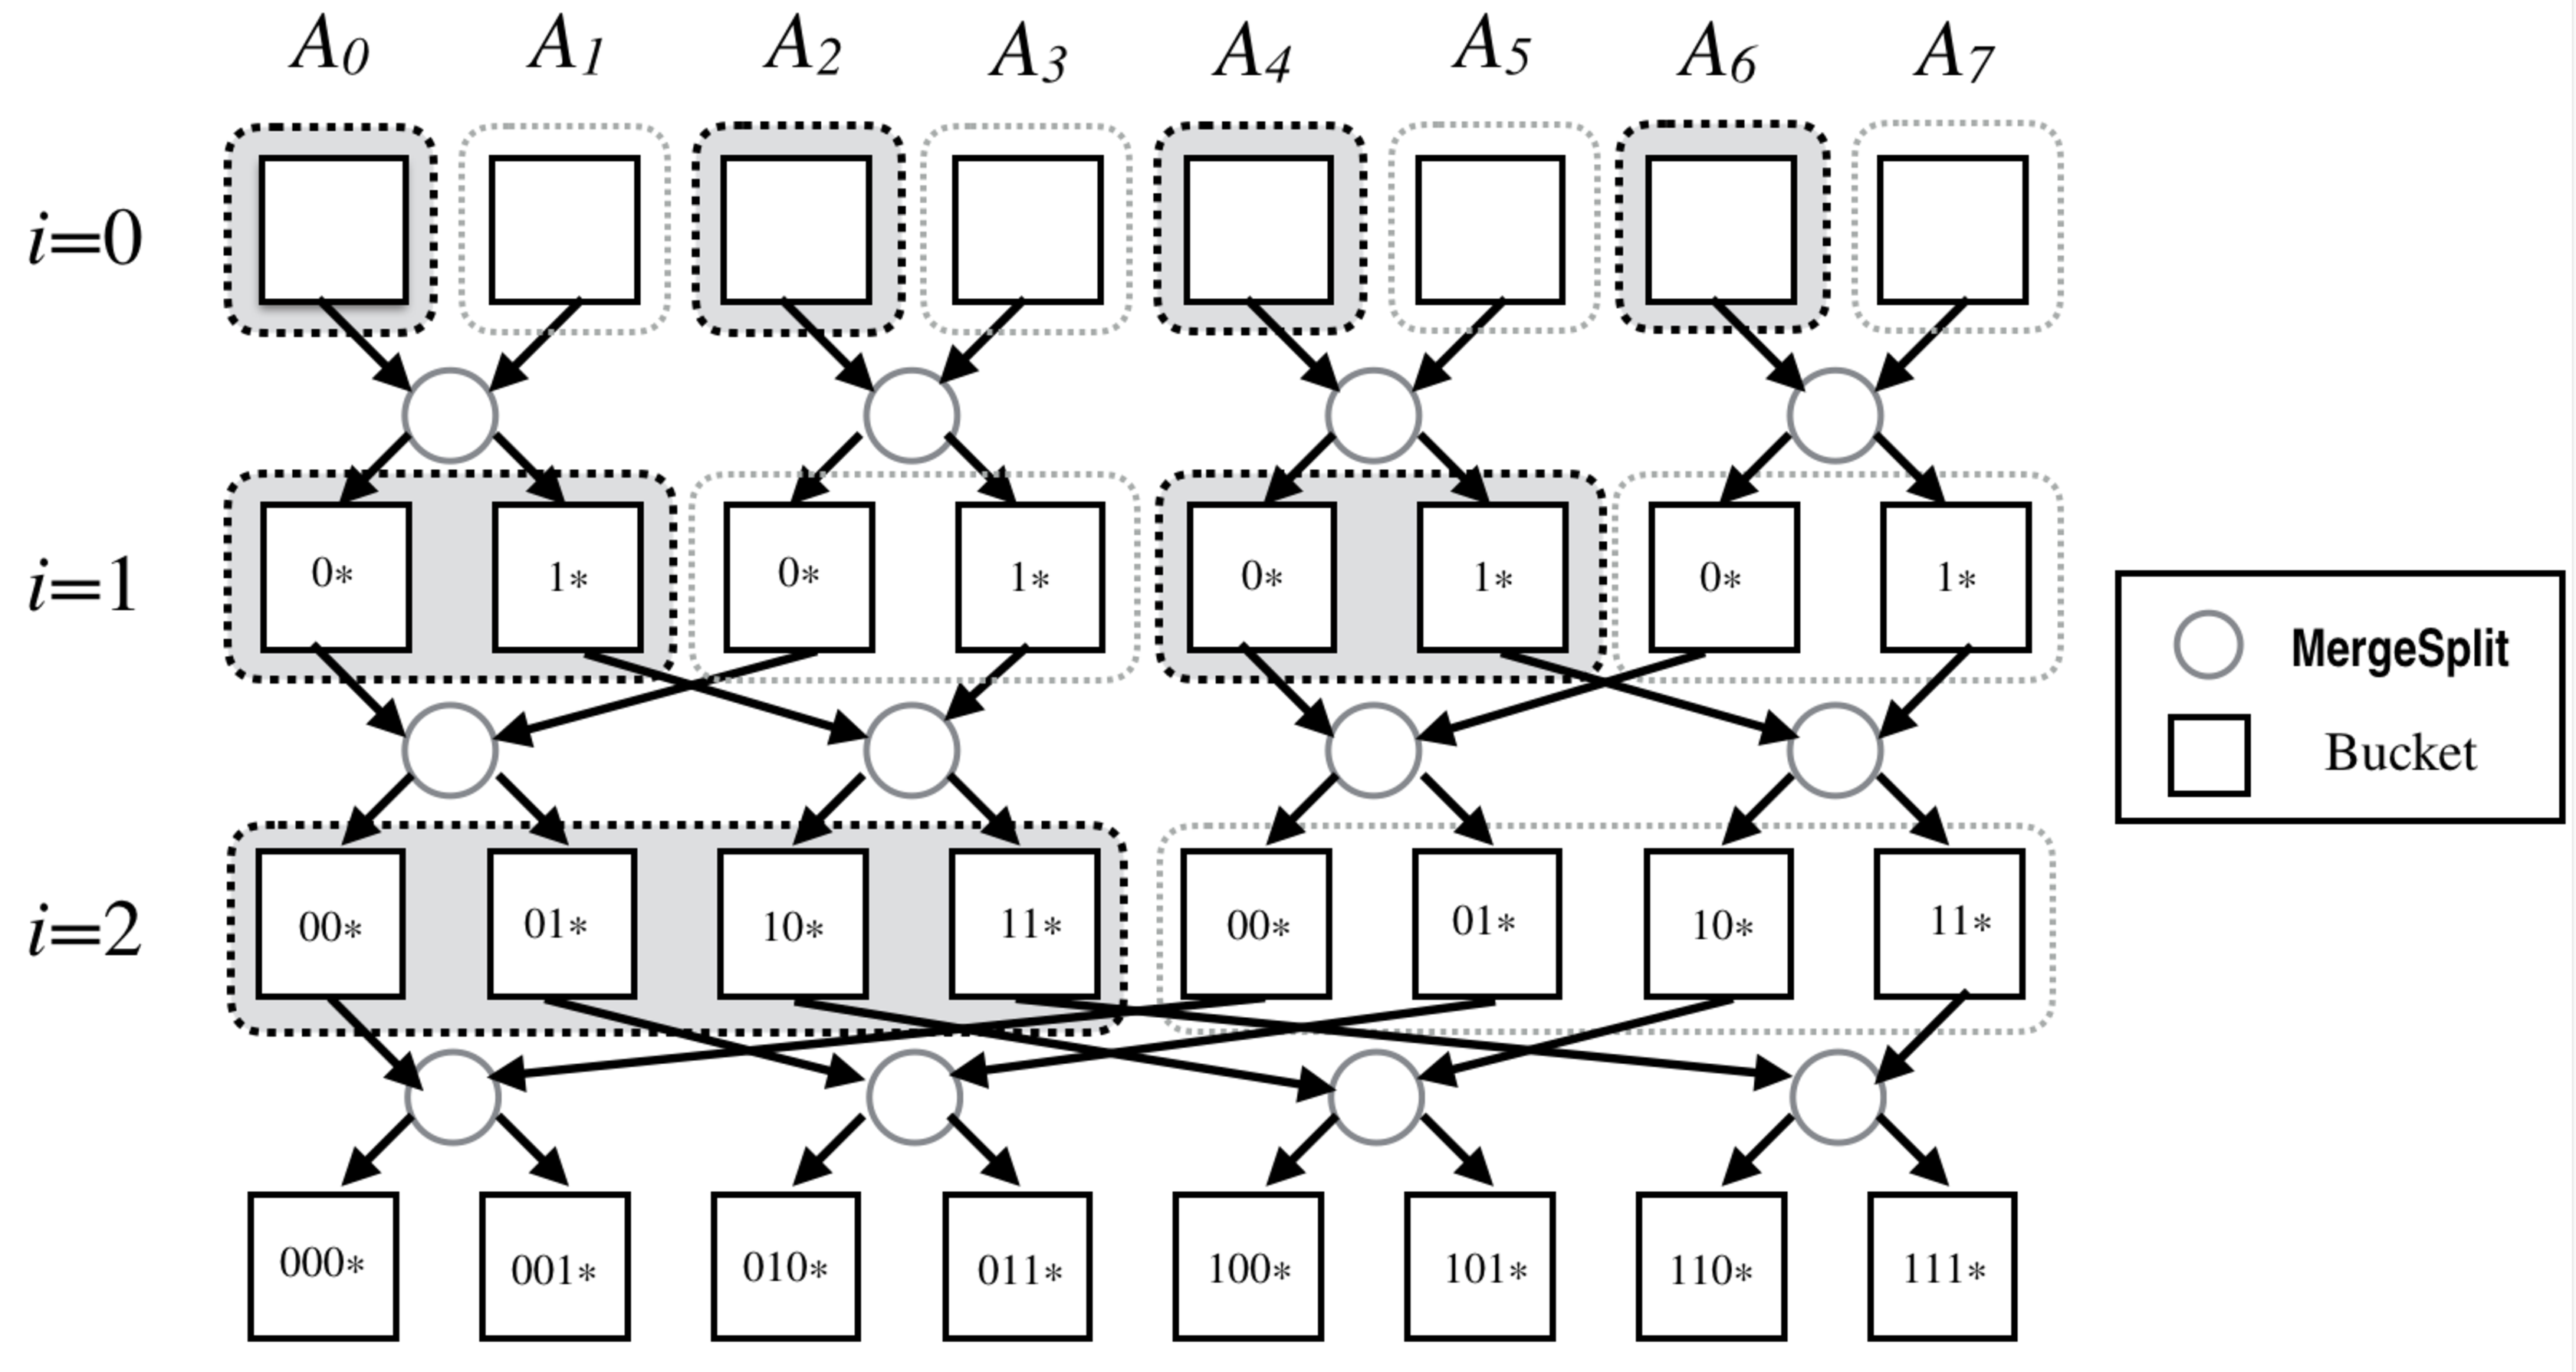
\includegraphics[width=0.7\textwidth]{RadixBucketSort1.pdf}
\captionof{figure}{\textbf{Oblivious random bin assignment with 8 buckets.}
The \textsc{MergeSplit} procedure takes elements from two buckets at level $i$ and put them into two buckets at level $i+1$, according to the $(i+1)$-th most significant bit of the keys. 
At level $i$, every $2^{i}$ consecutive buckets are semi-sorted by the most significant $i$ bits of the keys.}
\label{fig:radix-sort}

%\begin{table*}[t]
\bigskip
\centering
\begin{tabular}{|c|c|c|c|c|}
    \hline
    Algorithm & Oblivious & Client storage & Runtime & Error probability \\
    \hline
    Merge sort & No & $O(1)$ & $2n \log n$ & 0 \\
    Bitonic sort & Yes & $O(1)$ & $n\log^2 n$ & 0 \\
    AKS sort~\cite{aks} & Yes & $O(1)$ & $5.4\times10^7 \times n\log n$ & 0 \\
    Zig-zag sort~\cite{zigzag} & Yes & $O(1)$ & $8\times10^4 \times n\log n$ & 0 \\
    Randomized Shellsort~\cite{RandShellsort} & Yes & $O(1)$ & $24n\log n$ & $\approx n^{-3}$ \\
    \hline
    \textbf{Bucket oblivious sort} & Yes & $2Z$ & $6 n\log n$ & $\approx e^{-Z/6}$\\
    \textbf{Bucket oblivious sort} & Yes & $O(1)$ & $\approx 2n\log n \log^2 Z$ & $\approx e^{-Z/6}$ \\
    \hline   
\end{tabular}
\captionof{table}{\textbf{Runtime of bucket oblivious sort and
classic non-oblivious and oblivious sort algorithms.} Bitonic
sort requires $\frac 14 n \log^2 n$ comparisons. The number of comparisons for AKS
sort and zig-zag sort are cited from \cite{zigzag}. Runtime
represents the number of memory accesses, which is four times the
number of comparisons.}
\label{tab:compare}
%\end{table*}

\end{figure*}

The core of our algorithms is to assign each element to a random bin and then route the elements through a butterfly network to their assigned random bins. 
This part is inspired by Bucket ORAM~\cite{fletcher2015bucket}. 
In more detail, we divide the $n$ elements into $B=2n/Z$ buckets of size $Z/2$ each and add $Z/2$ dummy elements to each bucket.
Now, imagine that these $B$ buckets form the inputs of a butterfly network --- for simplicity, assume $B$ is a power of two.
Each element is uniformly randomly assigned to one of the $B$ output buckets, represented by a key of $\log B$ bits.
The elements are then routed through the butterfly network to their respective destinations.
Assuming the client can store two buckets locally at a time, at level $i$, the client simply reads elements from two buckets that are distance $2^i$ away in level $i$ and writes them to two adjacent buckets in level $i+1$, using the $i$-th bit of each element's key to make the routing decision. 
We refer readers to Figure~\ref{fig:radix-sort} for a graphical illustration.

The above algorithm is clearly oblivious, as the order in which the client reads and writes the buckets is fixed and independent of the input array. If no bucket overflows, all elements reach their assigned destinations. By setting $Z$ appropriately, we can bound the overflow probability.

Our bucket oblivious sort and bucket ORP algorithms are derived from
the above oblivious random bin assignment building block. 

\paragraph{From oblivious random bin assignment to ORP and oblivious sort.}
To obtain a random permutation, we simply remove all dummy elements and randomly permute 
each bucket of the final layer.
Since the client can hold $Z$ elements, permuting each bucket can be done locally. 
We show that the algorithm is oblivious and gives a random permutation despite revealing the number of dummy elements in each destination bucket.
To get oblivious sort, we can first perform ORP on the input array then apply any \emph{non-oblivious, comparison-based} sorting algorithm (e.g., quick sort or
merge sort). We show that the composition of ORP and non-oblivious sort results in an oblivious sort. 

\paragraph{Dealing with small client storage.}
In Section~\ref{sec:O1client}, we extend our algorithms to support $O(1)$ client storage. 
We can rely on bitonic sort to realize the \textsc{MergeSplit} operation that operates on 4 buckets at a time,
which would result in $O(n\log n\cdot \log^2 Z)$ runtime. 

\paragraph{Locality.} Algorithmic performance when the data is stored on disk has been studied in the external disk model (e.g.,~\cite{RuemmlerW94,ArgeFGV97,Vitter01,Vitter06}) and references within). Recently, Asharov et al.~\cite{AsharovCNPRS19} extended this study to oblivious algorithms.  We discuss how our algorithms can be made locality-friendly in Section~\ref{sec:locality}. 


%\paragraph{Organization.}
%The rest of the paper is organized as follows. Our algorithms are simple and intuitive. The access pattern of all our algorithms is deterministic, and therefore security is trivial and all we have to prove is correctness. In Section~\ref{sec:construction} we give our construction and in Section~\ref{sec:extensions} we describe simple extensions. In Appendix~\ref{sec:defs}  define the RAM model of computation and obliviousness. In Appendix~\ref{appx:formal} we give all omitted proofs. 

%
%
%\paragraph{From oblivious bin assignment to ORP.}
%To obtain a random permutation, a simple approach is to remove the dummy elements and permute within each bucket of the final layer. Since the client can hold $Z$ elements, permuting each bucket obliviously can be done locally. 
%
%
%Our bucket oblivious sort and bucket ORP build on top of the above oblivious random bin assignment. 
%To get ORP, simply remove all dummy elements, randomly permute each bucket of the final level, and concatenate the bins.
%To sort, we can simply apply any non-oblivious comparison-based sort (e.g., merge sort) on the randomly permuted elements. 
%
%In Section~\ref{sec:O1client}, we will discuss how to extend our algorithms to support constant client storage
%We can rely on Bitonic sort to realize the ${\bf MergeSplit}$ operation, which would result in $\approx 2n\log n \log^2 Z$ runtime.
%Recently, Asharov et al.~\cite{AsharovCNPRS19} initiate the study of data locality on oblivious algorithms. 
%We observe that our algorithms are be made locality-friendly, and refer readers to Appendix~\ref{sec:locality} for the exact definitions and complexity measures.

%%% Local Variables:
%%% mode: latex
%%% TeX-master: "main"
%%% End:

%!TEX root = main.tex

\newcommand{\memsize}{{N}}
\newcommand{\blocksize}{{b}}
%\newcommand{\negl}{{\sf negl}}
\newcommand{\Y}{{\bf Y}}

%\section*{Appendix}
%In the following we formally define the RAM model of computation, and formally prove obliviousness of our algorithms. 
%
\section{Preliminaries}
\label{sec:defs}

\paragraph{Notations and conventions.}
Let $[n]$ denote the set $\{1,\ldots,n\}$. Throughout this paper, we will use
$n$ to denote the size of the instance and use $\lambda$ to denote the security parameter. 
%A function $\negl$ is called \emph{negligible} if for any constant $c > 0$ and all sufficiently large $\sec$'s, it holds that $\negl < \sec^{-c}$. 
For an ensemble of distributions $\{D_\sec\}$ (parametrized with $\sec$),
we denote by $x \leftarrow D_\sec$ a sampling of an instance from the distribution $D_\sec$. 
We say two ensembles of distributions $\{X_\sec\}$~and~$\{Y_\sec\}$ 
are $\e(\sec)$-statistically-indistinguishable, denoted $\{X_\sec\} \overset{\e(\sec)}{\equiv} \{Y_\sec\}$, 
if for any unbounded adversary $\A$, 
\[
\left|\Pr_{x\leftarrow X_\sec}\left[\A(1^\lambda, x)=1\right] - \Pr_{y\leftarrow Y_\sec}\left[\A(1^\lambda, y)=1\right] \right| \leq \e(\sec) \ .
\]


%For simplicity, we will omit writing the unary security parameter input $1^\lambda$ to all procedures.
%\rl{We are writing the unary security parameter at a lot of places now. Should we add it everywhere and remove this statement?}
% Also, \emph{work} (or bandwidth) is always specified in terms of number of blocks of size $\Omega(\log N)$ accessed.

%\subsection{Memory with Multiple Disks and Data Locality}
%\label{sec:modeling-locality-formal}
%%\paragraph{Random-access machines.}
%%A RAM is an interactive Turing machine that consists of a memory and a CPU.  The
%%memory is denoted as $\mem[N,\bsize]$, and is indexed by the logical
%%address space $[N] = \{1,2,\ldots,N\}$. We refer to each memory word also as a
%%\emph{block} and we use $\bsize$ to denote the bit-length of each block. The CPU
%%has an internal state that consists of $O(1)$ words. The memory supports read/write
%%instructions $(\op,\addr, \data)$, where $\op \in \{\Read,\Write\}$, $\addr \in
%%[N]$ and $\data \in \bit^\bsize \cup \{\bot\}$.  If $\op = \Read$, then
%%$\data=\bot$ and the returned value is the content of the block located in
%%logical address $\addr$ in the memory. If $\op=\Write$, then the memory data in
%%logical address $\addr$ is updated to $\data$.
%%
%%
%%\paragraph{Locality.}
%%We model locality by dividing the memory address space $[N]$ to $\disks$ disks, simply by dividing the memory space to $\disks$ 
%
%
%% \kartik{define bandwidth?}
%To understand the notion of data locality, it may be convenient
%to view the memory as $\disks$ rotational hard drives or other
%storage mediums where sequential accesses are faster than random
%accesses. The program interacting with the memory has to specify
%which disk to access.  
%Each disk is equipped with one read/write head. In order to serve
%a $\Read$ or $\Write$ request with address $\addr$ in some disk
%$\disk \in [\disks]$, the memory has to move the read/write head
%of the disk $\disk$ to the physical location $\addr$ to perform
%the operation.  
%Any such movement of the head introduces cost and delays,  
%and the machine that interacts with the memory would like to
%minimize the  number of move head operations. 
%Traditionally, the latter can be improved by 
%ensuring that the program accesses contiguous regions of the
%memory. 
%% storing related
%% items to physically proximate areas on the memory.  
%However, this poses a great challenge for oblivious computation
%in which data is often continuously shuffled across memory.  
%
%More formally, a memory is denoted as $\mem[N,\bsize,\disks]$,
%consisting of $\disks$ disks, indexed by the address space $[N] =
%\{1,2,\ldots,N\}$, where $\disks \cdot N$ is the size of the
%logical memory. We refer to each memory word also as a
%\emph{block} and we use $\bsize$ to denote the bit-length of each
%block.  
%The memory supports the following two types of instructions.
%\begin{MyItemize}
%\item {\bf \boldmath Move head operation} $(\move,\disk,\addr)$
%moves the head of the $\disk$-th disk ($\disk \in [\disks]$) to point to address $\addr$ within that disk. 
%
%\item {\bf \boldmath A read/write operation} $(\op,\disk,\data)$, 
%where $\op \in \{\Read,\Write\}$, $\disk \in [\disks]$ and $\data \in \bit^\bsize \cup \{\bot\}$. 
%If $\op = \Read$, then $\data=\bot$ and $\mem$ should return the content of the block pointed to by the $\disk$-th disk; 
%If $\op=\Write$, the block pointed to by the $\disk$-th disk is updated to $\data$. The $\disk$-th head is then incremented to point to the next consecutive address, and wrapped around when the end of the disk is reached. 
%
%\end{MyItemize}
%
%\medskip
%\noindent
%{\bf Locality.}
%%\paragraph{Locality.}
%% The number of $\move$ operations defines locality.
%A sequence of memory operations has $(\disks,
%\locparam)$-locality if it contains $\locparam$ $\move$
%operations to a memory that is equipped with $\disks$ disks.  
%
%
%\medskip
%\noindent
%{\bf Relation to the standard memory definition.}
%%\paragraph{Relation to the standard memory definition.} 
%Instead of specifying which disk to read from/write to, we can define a memory of range $[\disks\cdot N] = \{1,\ldots,\disks\cdot N\}$. 
%The address space determines the disk index, and therefore also
%whether or not to move the read/write head. Thus, one can
%consider the regular notion of a RAM program, and our definition
%provides a way to measure the locality of the program. Different implementations
%of the same  functionality can have different locality, similarly to other metrics.

\paragraph{Random-access machines.}
A RAM is an interactive Turing machine that consists of a memory and a CPU.  The
memory is denoted as $\mem[\memsize,\blocksize]$, and is indexed by the logical
address space $[N] = \{1,2,\ldots,N\}$. We refer to each memory word also as a
\emph{block} and we use $\bsize$ to denote the bit-length of each block. The memory supports read/write
instructions $(\op,\addr, \data)$, where $\op \in \{\Read,\Write\}$, $\addr \in
[N]$ and $\data \in \bit^\bsize \cup \{\bot\}$.  If $\op = \Read$, then
$\data=\bot$ and the returned value is the content of the block located in
logical address $\addr$ in the memory. If $\op=\Write$, then the memory data in
logical address $\addr$ is updated to $\data$.
We use standard setting that $\blocksize = \Theta(\log N)$ (so a word can 
store an address).
%We follow the convention that the CPU performs one \emph{word-level operation} per unit time,
%i.e., arithmetic operations (addition or subtraction), 
%bitwise operations (AND, OR, NOT, or shift), memory accesses (read or write), or
%evaluating a pseudorandom function~\cite{oram00,oram09,oram03,oblivhash,LarsenN18,panorama}.

\medskip
\noindent
{\bf Obliviousness.}
Intuitively, a RAM program $M$ obliviously simulates a RAM program $f$ if: (1) it has the same input/output behavior as $f$; (2) There exists a simulator $\Sim(\abs{x})$ that produces access pattern that is statistically close to the access pattern of $M(x)$, i.e., it can simulate all memory addresses accessed by $M$ during the execution on $x$, without knowing $x$. In case the access pattern and the functionality are randomized, we have to consider the joint distribution of the simulator and the output of the RAM program or the functionality. 

%In our sorting algorithm, the access pattern is randomized but the functionality is deterministic. In the oblivious random permutation algorithm, the access pattern is deterministic but the functionality is randomized. As always either the access pattern or the functionality is deterministic, we can consider a simpler definition of obliviousness in which the functionality and the simulation are considered separately. 

For a  RAM machine $M$ and input $x$, let ${\sf AccPtrn}(M(x))$ denote the distribution of memory addresses a machine $M$ produces on an input $x$.
\begin{definition}
A RAM algorithm $M$ obliviously implements the functionality $f$ with $\e$-obliviousness if the following hold:
\begin{eqnarray*}
\left\{\Sim(1^\lambda),f(x)\right\}_{x \in \bit^\lambda} \overset{\epsilon(\lambda)}{\equiv} \left\{ {\sf AccPtrn}(M(x)),M(x)\right\}_{x \in \bit^\lambda}
\end{eqnarray*}
If $\epsilon(\cdot)=0$, we say $M$ is perfectly oblivious. 
%\[ \left\{\Sim(1^\lambda),f(x)\right\}_{x \in \bit^\lambda} 
%\overset{\epsilon(\lambda)}{\equiv} \left\{ {\sf AccPtrn}(M(x)),M(x)\right\}_{x \in \bit^\lambda} \]
\end{definition}

%$$
%$$
%\begin{MyItemize}
%
%\item {\bf $\delta$-Correctness:} For every input $x$ it holds that 
%$$
%\Pr\left[M(x) = f(x) \right] \geq 1- \delta(\abs{x})
%$$
%
%\item {\bf $\e$-Obliviousness:} There exists a simulator $\Sim(\abs{x})$ such that
%$$
%\left\{{\sf AccPtrn}(M(x))\right\}_{\abs{x}} \overset{\e(\abs{x})}{\equiv} 
%\left\{\Sim(\abs{x})\right\}_{\abs{x}}
%$$
%%that produces access pattern that is statistically close to the access pattern of $M(x)$.
%\end{MyItemize}
%\end{definition}

%A functionality $f$ is a (possibly randomized) RAM machine that gets some input $x$ and computes an output $y$. A RAM algorithm $M$ obliviously implements the functionality $f$ if: (1) it has the same input/output behavior as $f$; (2) There exists a simulator $\Sim(\abs{x})$ that produces access pattern that is statistically close to the access pattern of $M(x)$. I.e., it can simulates all memory addresses accessed by $M$ during the execution on $x$, without knowing $x$. Note that all our algorithms have deterministic access pattern, and therefore 
%
%In case where the functionality $f$ is randomized, we require that the joint distribution of the output of the functionality and the output of the simulator would be statistically close to the output of the algorithm $M$ and its access pattern. Formally, we let ${\sf AccPtrn}(M(x))$ denote the distribution of memory addresses a machine $M$ produces on an input $x$. We have:
%
%\begin{definition}[Oblivious machines]
%\label{defn:omachine}
%Let $f,M:\bit^* \rightarrow \bit^*$ be (possibly randomized) RAM programs. We say that $M$ {\em obliviously simulates $f$} if there exists a  simulator $\Sim$ and a negligible function $\epsilon(\cdot)$ such that  for any $\lambda$:% and any input $x$ of size $\lambda$ it holds that:
%\begin{eqnarray*}
%\hspace{-5ex}\lefteqn{\left\{\Sim(1^\lambda),f(x)\right\}_{x \in \bit^\lambda}} \\
%&&\hspace{+5ex}\overset{\epsilon(\lambda)}{\equiv} \left\{ {\sf AccPtrn}(M(x)),M(x)\right\}_{x \in \bit^\lambda}
%\end{eqnarray*}
%If $\epsilon(\cdot)=0$, we say $M$ is perfectly oblivious. 
%\end{definition}

The two main functionalities that we focus on in this paper are the following:

\paragraph{Oblivious sort:}
This is a deterministic functionality in which the input is an array $A[1,\ldots,n]$ of memory blocks (i.e., each $A[i] \in \bit^\blocksize$, representing a key). The goal is to output an array $A'[1,\ldots,n]$ which is some permutation $\pi:[n] \rightarrow [n]$ of the array $A$, i.e., $A'[i] = A[\pi(i)]$, such that $A'[1]\leq \ldots \leq A'[n]$. %Obliviousness is defined using Definition~\ref{defn:omachine}. We denote this functionality as ${\cal F}_{\rm sort}$. 

\paragraph{Oblivious permutation:} 
This is a randomized functionality in which the input is an array $A[1,\ldots,n]$ of memory blocks. The functionality chooses a random permutation $\pi:[n] \rightarrow [n]$ and outputs an array $A'[1,\ldots,n]$ such that $A'[i] = A[\pi(i)]$ for every $i$. %Obliviousness is defined using %Definition~\ref{defn:omachine}. Note that the definition requires that the access pattern does not leak the permutation chosen by the functionality. We denote this functionality ${\cal F}_{\rm perm}$. 
%\end{MyItemize}


%\section{Obliviousness}
%\label{appx:formal}
%In this section we provide proofs for obliviousness of our constructions. In Section~\ref{sec:rand:functionality} we formally define the ideal functionality of the random bin assignment (Algorithm~\ref{code:obin}). 
%
%
%\subsection{\boldmath Random Bin Assignment: Functionality}
%\label{sec:rand:functionality}
%We start with defining the oblivious random bin assignment functionality, which we denote by $f_{\rm randbin}$. In a nutshell, given some input array ${\bf X}$ we consider an output array which has twice the size of the input array, and we consider the output array as $B$ consecutive bins. We assign each ``real'' element of the input array into a random bin in the output array, and pad each bin with dummy elements. We will show how to realize the functionality for $Z := \alpha \log \lambda$ with $\alpha \in \omega(1)$ and $\lambda$ is the security parameter. 
%
%
%\begin{myfunc}
%[\boldmath ${\cal F}_{\rm randbin}(\X,Z)$]
%\label{func:bin-assignment}
%The random bin assignment functionality ${\cal F}_{\rm randbin}(\X,Z)$ is defined as follows:
%\begin{MyItemize}
%\item {\bf Input:} an input an array $\X$ of length $n$ containing real and dummy elements, and a bin size~$Z$. 
%\item {\bf The functionality:} 
%\begin{MyEnumerate}
%\item Define an output array $\Y$ of size $2n$, containing $B = 2n/Z$ bins of size $Z$ each, denoted as $\Y_1,\ldots,\Y_B$. 
%\item For every real element in $\X$ choose a random destination bin $i \gets [B]$, and place the element in the $i$th output bin. 
%\item If some output bin contains more than $Z$ elements, then {\sf abort}. 
%\item Pad each output bin to its maximal capacity using dummy elements. Order each output bin as follows: 
%(1) all real elements appear before dummies;
%and (2) real elements are ordered according to their ordering (indices) in the input array $\X$.
%\end{MyEnumerate}
%\end{MyItemize}
%\end{myfunc}
%
%
%\begin{lemma}
%Let $Z = \alpha \log \lambda$ for any super-constant function $\alpha(\lambda)$.
%Algorithm~\ref{code:obin}
%obliviously simulates ${\cal F}_{\rm randbin}$ (i.e., Functionality~\ref{func:bin-assignment}) with $\epsilon(n, Z) = 2n/Z \cdot \log(2n/Z) \cdot e^{-Z/6}$ failure probability. %The algorithm completes in $O(\frac{n}{Z}\log n \cdot T_{\sf MergeSplit}(Z))$ work, where $T_{\sf MergeSplit}(Z)$ .
%\label{lem:randbin}
%\end{lemma}
%\begin{proof}
%The access pattern of Algorithm~\ref{code:obin} is deterministic and is independent of the input, and therefore it can be simulated easily. Moreover, since it is deterministic, it suffices to consider correctness and access pattern separately, and there is no need to consider the joint distribution. 
%As for correctness, we claim that the algorithm implements Functionality~\ref{func:bin-assignment}. Specifically, the functionality and the algorithm choose the same bin assignment for all elements with the exact same probability. Moreover, for the same bin assignments for all elements, the functionality and the algorithm result in the same output, except for a negligible probability of failure. This occurs when there is some internal overflow in the algorithm in one of the iterations $i \in \{1,\ldots,\log B\}$, which does not occur in the functionality. 
%%As for efficiency, we run ${\sf MergeSplit}$ exactly $B \log B$ times, which results in $O(\frac{n}{Z}\log n \cdot T_{\sf MergeSplit}(Z))$. 
%%	%Sorting each bin results in $B \cdot (Z \log^2 Z) = n \log^2 Z$, which is smaller than $O(n \log n)$. 
%\end{proof}
%%
%%\subsection{Oblivious Sort from Oblivious Random Bin Assignment}
%%\label{sec:obliviousSortFromRandomBinAssignment}
%%
%%We formalize the composition theorem: Given an oblivious random bin assignment, 
%%%\paragraph{Oblivious sort from random bin assignment algorithm  and non-oblivious sort.}
%%Given a random bin assignment algorithm 
%%${\sf ObliviousRandomBin}$ and a non-oblivious
%%comparison-based sorting algorithm ${\sf NonObliviousSort}$ (e.g., Merge-Sort), one can 
%%easily construct
%%an oblivious sorting algorithm as follows. 
%%%
%%\begin{myalgorithm}
%%[${\sf ObliviousSortFromRandomBinAssignment}(\X)$]
%%\label{alg:sort-from-random-bin}
%%\leavevmode
%%\begin{MyEnumerate}%[leftmargin=5mm]
%%\item 
%%Given an input array $\X$, invoke the random bin assignment algorithm to receive $\Y: = {\sf ObliviousRandomBin}(\X)$. Note that in each ``bin'' of $\Y$, the real elements appear before the dummy elements, and are sorted. Moreover, $\abs{\Y}=2\abs{\X}$.  
%%
%%%\item Obliviously sort each bucket $A_0,\ldots,A_{B-1}$ using Bitonic Sort, sorting the real elements according to their keys, and preferring real elements over dummy elements. 
%%
%%
%%\item Sort $\Y$ using a (non-oblivious) comparison-based sorting algorithm. 
%%That is, invoke ${\Y'} := {\sf NonObliviousSort}(\Y)$, while preferring real elements over dummy elements. 
%%Formally speaking, a sorting algorithm is comparison-based if the physical access pattern depends only on the relative ranking of elements in the input. 
%%A technical condition we need is that no two elements have the same rank. This can be ensured by resolving any tie consistently by the initial location of the elements in the array $\Y$.
%%
%%\item Now, all dummy elements appear at the $n$ last locations of $\Y'$. Truncate the last $n$ elements of $\Y'$. 
%%
%%\end{MyEnumerate}
%%\end{myalgorithm}
%%
%%%Let ${\sf Truncate}$ denote the last step of the above algorithm. Then, our sorting algorithm can be described as the following simple composition 
%%%$$ {\sf Truncate}({\sf NonObliviousSort}({\sf ObliviousRandomBin}(\X))) \ .$$
%%
%%\paragraph{Why is it oblivious?} 
%%Given that we do not fully permute the input array, a natural question is why the above composition is still oblivious. Essentially, the composition still holds since there is a 1-to-1 mapping between any input of the array and every possible output of the ${\cal F}_{\rm randbin}$ functionality, i.e., every possible input of the non-oblivious sorting algorithm. This mapping is exactly the random assignment of the destination bins. Therefore,  every access pattern in the non-oblivious sorting part of the algorithm, can be justified with some specific random assignment on the input array, for every possible ordering of the input array. However, some of the  assignments are ``invalid'' due to overflows; yet, overflows occur with negligible probability, and therefore we get statistical security. We proceed to the formal proof of security:
%%
%%\begin{lemma}[From oblivious random bin to oblivious sort]
%%Suppose that {\sf ObliviousRandomBin} is a statistically (or perfectly resp.)
%%oblivious random bin assignment algorithm.
%%Then, 
%%the above algorithm is a statistically (or perfectly resp.) secure 
%%oblivious sorting algorithm. 
%%\label{lem:orpsort}
%%\end{lemma}
%%\begin{proof}
%%Since the functionality is deterministic, we can consider obliviousness and correctness separately. Correctness of the algorithm is trivial. 
%%We next prove the obliviousness of the algorithm. 
%%We prove for the case of perfect security, since statistical security is similar,
%%except that we replace ``identically distributed'' with ``statistically close''.
%%
%%
%%Let ${\sf SimRandBin}$ be the simulator algorithm for 
%%the underlying oblivious random bin assignment.
%%Consider any given input $\X$ of length $n$, 
%%and let $(\Y, {\sf addressesRandBin})$ 
%%denote the joint distribution of the outcome array $\Y$ and the addresses
%%accessed during an execution of the oblivious random bin assignment.
%%Lemma~\ref{lem:randbin} implies that:
%%$$
%%\left(\Y, {\sf addressesRandBin}\right) \equiv \left({f}_{\rm randbin}(\X), {\sf SimRandBin}(1^n,|\X|)\right)  \ . \vspace{-1ex}
%%$$
%%Let ${\sf SortAddresses}(\Y)$ 
%%denote the addresses observed during an execution 
%%of the truncation algorithm and the non-oblivious, comparison-based 
%%sorting algorithm upon receiving input array $\Y$.
%%We thus have that\vspace{-1ex}
%%\begin{eqnarray*}
%%\hspace{-15ex}\lefteqn{\left({\sf SortAddresses}(\Y), {\sf addressesRandBin}\right)}\\
%%&& \hspace{+15ex}\equiv 
%%\left({\sf SortAddresses}({f}_{\rm randbin}(\X)), {\sf SimRandBin}(1^n,|\X|)\right) \ .   \vspace{-1ex}
%%\end{eqnarray*}
%%For any comparison-based 
%%sort, its access patterns depend only on 
%%the relative ranking of the input elements. Since without loss of generality, 
%%we assumed that the input array $\X$ always has distinct values, and we carefully defined how to avoid any ties, 
%%we have that\vspace{-1ex}
%%$$
%%{\sf SortAddresses}({f}_{\rm randbin}(\X)) \equiv
%%{\sf SortAddresses}({f}_{\rm randbin}([|\X|])) \ , \vspace{-1ex}
%%$$
%%where $[|\X|] = \{1,\ldots,|\X|\}$. 
%%Now, 
%%observe that we can construct a simulator 
%%${\sf SimObliviousSort}$
%%that simply outputs 
%%$$
%%{\sf SortAddresses}({f}_{\rm randbin}([|\X|])), {\sf SimRandBin}(1^n,|\X|)
%%$$
%%This simulator's output is identically distributed
%%as the real-world access patterns of executing
%%the aforementioned sorting algorithm, i.e., to $({\sf SortAddresses}(\Y), \allowbreak{\sf addressesRandBin})$. 
%%\end{proof}
%%
%%%We therefore conclude:
%%%\begin{corollary}
%%%\label{cor:rand-bin-using-bitonic}
%%%Let $Z = \alpha \log \lambda$ for any super-constant function $\alpha(\lambda)$, and assume that a client can store $4\cdot Z$ elements locally. 
%%%Algorithm~\ref{alg:bucket-sort}, where ${\sf MergeSplit}$ 
%%%obliviously simulates ${\cal F}_{\rm randbin}$ (i.e., Functionality~\ref{func:bin-assignment}) with $\negl$ statistical 
%%%failure. The algorithm completes in $O(n \log n)$ work.
%%%\end{corollary}
%%
%%%\medskip
%%%\noindent
%%%{\bf Building blocks.} Moreover, in Appendix~\ref{sec:building-blocks} we review some building blocks that we will use in our construction, including oblivious sorts, {\sf Dedup} -- an algorithm that removes duplicates obliviously based on oblivious sorts, and Oblivious Bin Packing -- an algorithm that receives an array as an input, where each element is marked with some destination bin, and the algorithm obliviously routes the elements into the bin, while padding each bin to its maximal capacity with dummy elements. This is again implemented using oblivious sorts. See Appendix~\ref{sec:building-blocks} for further details.   
%%
%%%%% Local Variables:
%%%%% mode: latex
%%%%% TeX-master: "main"
%%%%% End:

%!TEX root = main.tex




\section{Our Construction} 
\label{sec:construction}
\label{sec:random-bin-assignment}

We first present the oblivious random bin assignment algorithm (Section~\ref{sec:obin})  and then use it to implement our bucket oblivious random permutation (Section~\ref{sec:ORP}) and bucket oblivious sort (Section~\ref{sec:osort}).

\newcommand{\val}{{\sf value}}
\newcommand{\pref}{{\sf pref}}

\begin{figure*}[h!]
\centering

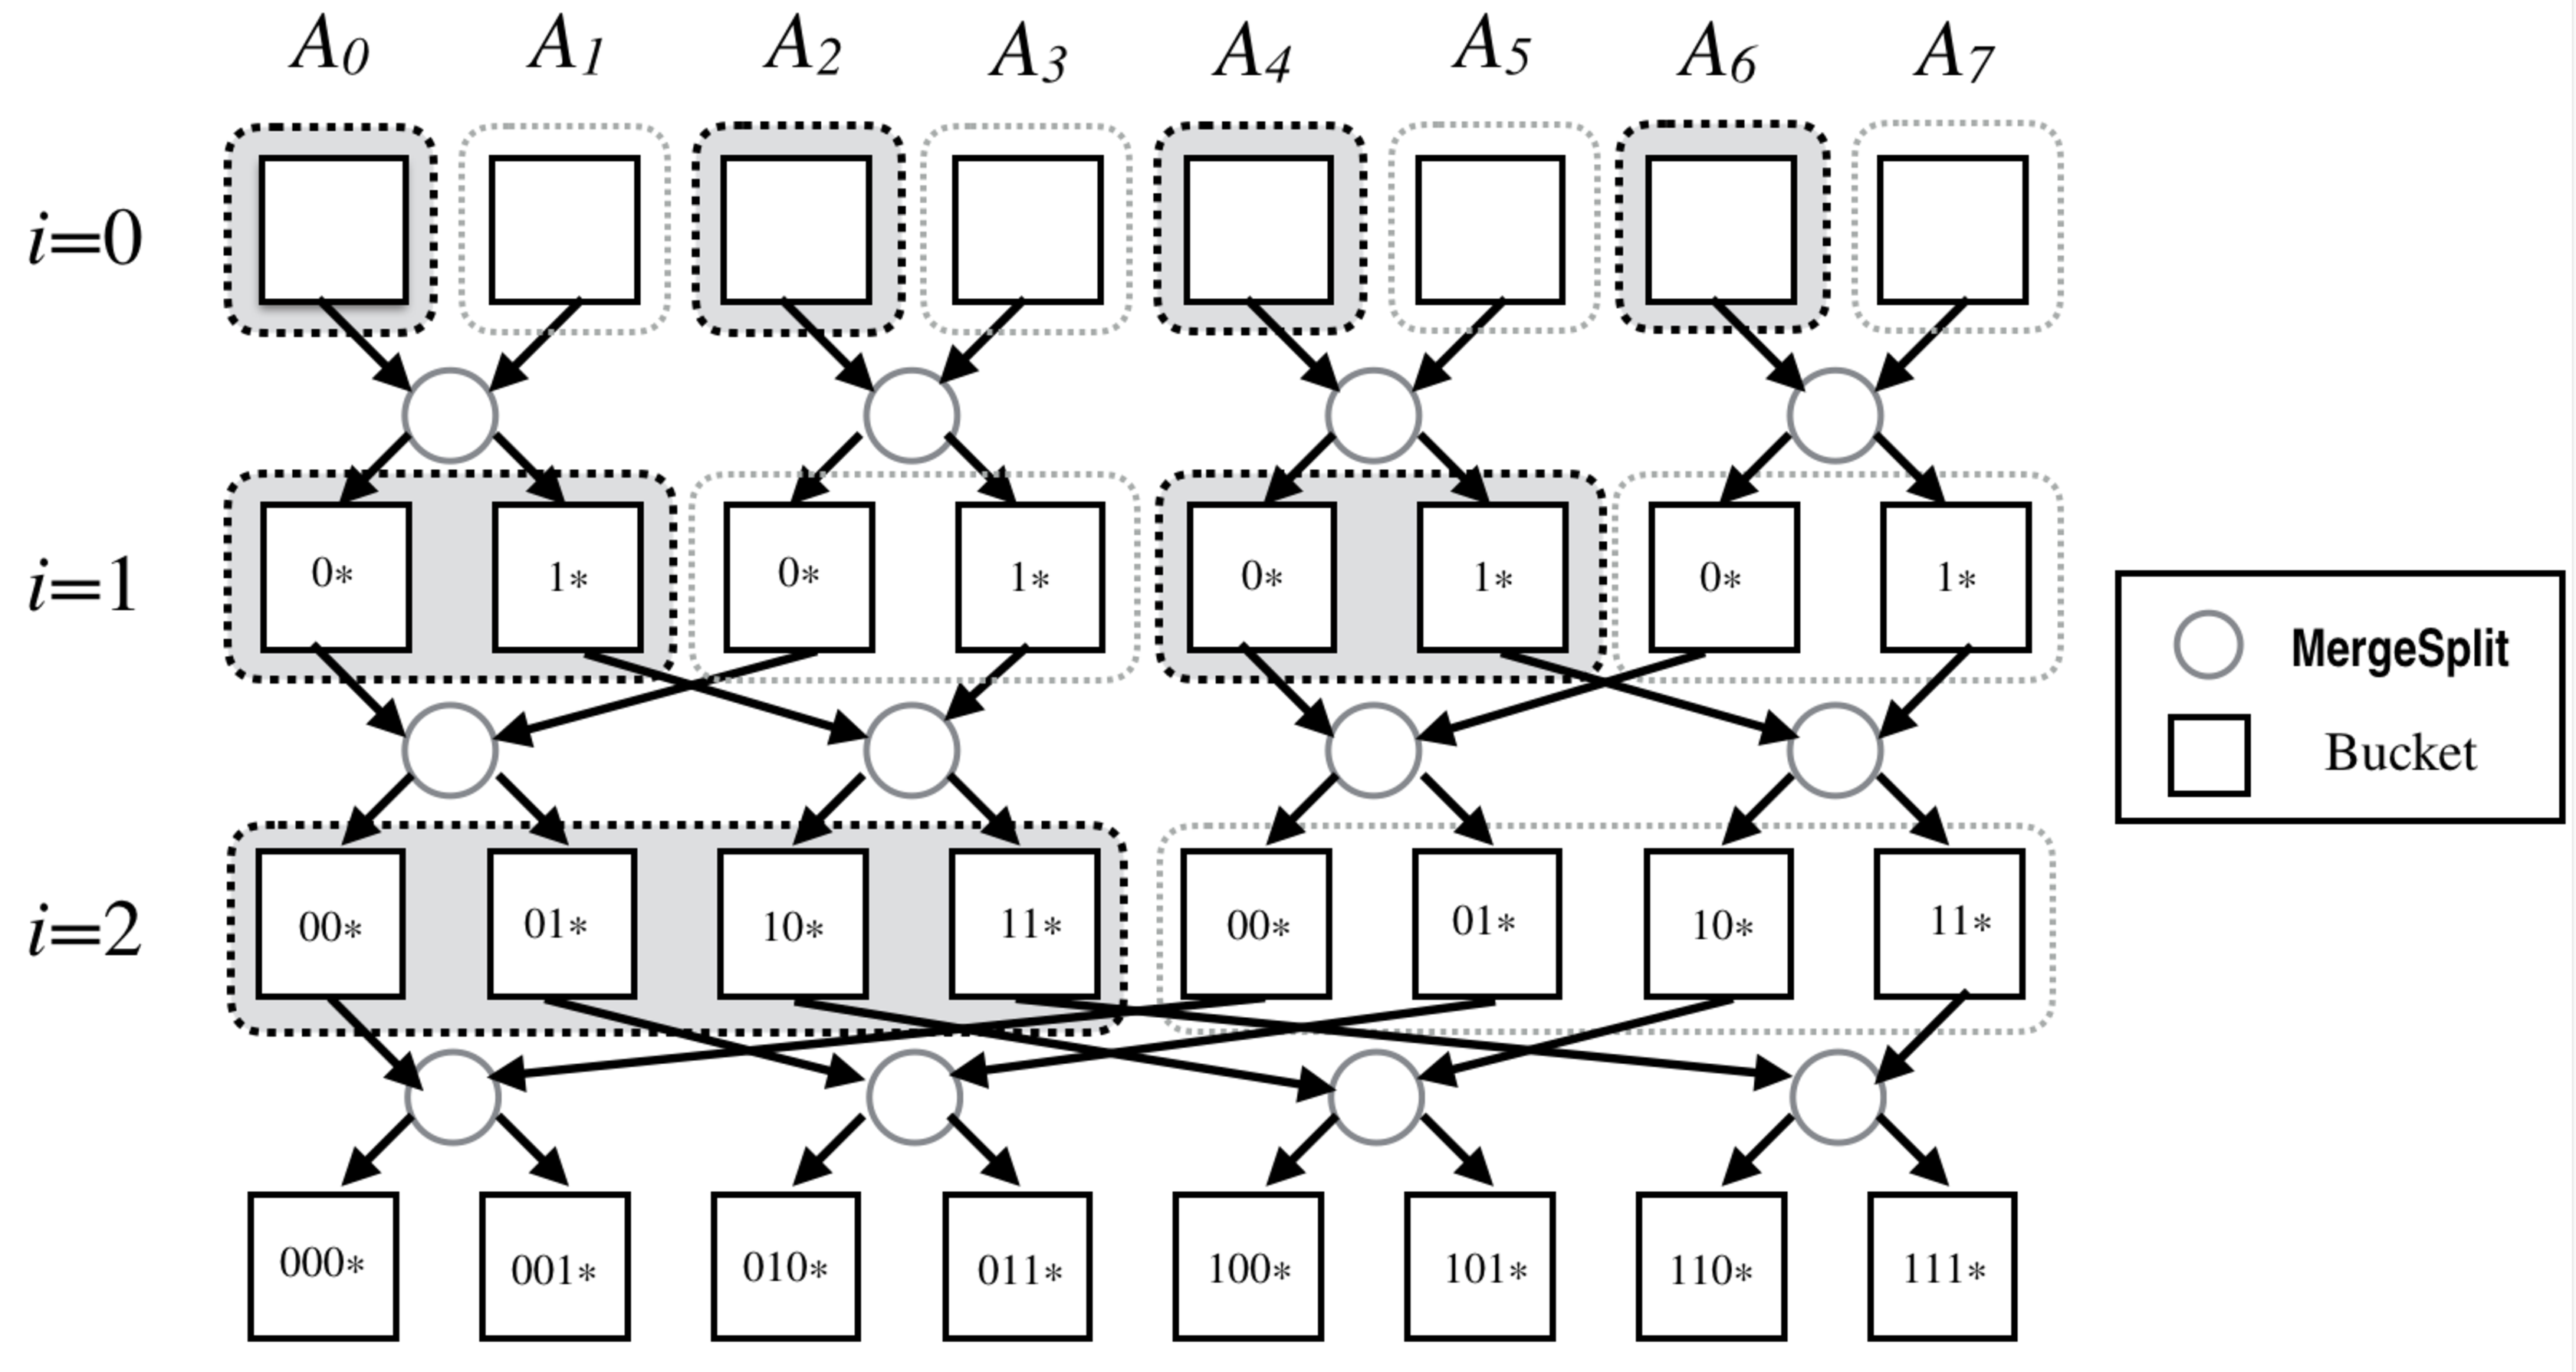
\includegraphics[width=0.75\textwidth]{RadixBucketSort1.pdf}
\captionof{figure}{Oblivious random bin assignment with 8 buckets.}
%The \textsc{MergeSplit} procedure takes elements from two buckets at level $i$ and put them into two buckets at level $i+1$, according to the $(i+1)$-th most significant bit of the keys. 
%At level $i$, every $2^{i}$ consecutive buckets are semi-sorted by the most significant $i$ bits of the keys.
\label{fig:radix-sort}

\bigskip
\begin{algorithm}[Oblivious Random Bin Assignment]
\begin{algorithmic}
\State
\State \textbf{Input}: an array $\X$ of size $n$
\State Choose a bucket size $Z$ and let $B$ be the smallest power of two that is $\geq 2n/Z$. 
\State Define $(\log B+1)$ arrays, each containing $B$ buckets of size $Z$. Denote the $j$-th bucket of the $i$-th array $A_j^{(i)}$.
\State For each element in $\X$, assign a uniformly random key in $[0,B-1]$.
\State Evenly divide $\X$ into $B$ groups. Put the $j$-th group into $A_j^{(0)}$ and pad with dummy elements to have size $Z$.

\For {$i=0,\ldots,\log B-1$}
    \For {$j=0,\ldots,B/2$}
        \State $(A^{(i+1)}_{2j}, A^{(i+1)}_{2j+1}) \leftarrow \textsc{MergeSplit}(A^{(i)}_{j'+j}, A^{(i)}_{j'+j+2^i}, i)$ where $j'=\lfloor j / {2^i} \rfloor \cdot 2^{i+1}$
        \State \Comment{Input: $j$-th pair of buckets with distance $2^i$ in $A^{(i)}$; Output: $j$-th pair of buckets in $A^{(i+1)}$}
        %\State Let $(A_0, A_1$) be the $j$-th pair of buckets with distance $2^i$ in $A^{(i)}$ 
        %\State Let $(A'_0, A'_1)$ be the $j$-th pair of buckets in $A^{(i+1)}$
        %\State $(A'_0, A'_1) \leftarrow \textsc{MergeSplit}(A_0, A_1, i)$ 
        
    \EndFor
\EndFor    
\State \textbf{Output:} $A^{(\log B)}$

\medskip
\Function{$(A'_0, A'_1) \leftarrow$ MergeSplit}{$A_0, A_1, i$}
    \State $A'_0$ receives all real elements in $A_0 \cup A_1$ where the $(i+1)$-st MSB of the key is $0$   
    \State $A'_1$ receives all real elements in $A_0 \cup A_1$ where the $(i+1)$-st MSB of the key is $1$
    \State If either $A'_0$ or $A'_1$ receives more than $Z$ real elements, the procedure aborts with {\sf overflow}
    \State Pad $A'_0$ and $A'_1$ to size $Z$ with dummy elements and return $(A'_0, A'_1)$
\EndFunction   
\end{algorithmic}
\label{code:obin}
\end{algorithm}

\bigskip
%\begin{table*}[t]
\centering
\begin{tabular}{|c|c|c|c|c|}
    \hline
    Algorithm & Oblivious & Client storage & Runtime & Error probability \\
    \hline
    merge sort & no & $O(1)$ & $2n \log n$ & 0 \\
    Bitonic sort & yes & $O(1)$ & $n\log^2 n$ & 0 \\
    AKS sort & yes & $O(1)$ & $5.4\times10^7 \times n\log n$ & 0 \\
    Zigzag sort & yes & $O(1)$ & $8\times10^4 \times n\log n$ & 0 \\
    Randomized Shellsort & yes & $O(1)$ & $24n\log n$ & $\approx n^{-3}$ \\
    \hline
    \textbf{Bucket oblivious sort} & yes & $2Z$ & $6 n\log n$ & $\approx e^{-6/3}$\\
    \textbf{Bucket oblivious sort} & yes & $O(1)$ & $2n\log n \log^2 Z$ & $\approx e^{-6/3}$ \\
    \hline   
\end{tabular}
\captionof{table}{Runtime of bucket oblivious sort and classic non-oblivious and oblivious sort algorithms.}
\label{tab:compare}
%\end{table*}

\end{figure*}
\subsection{Oblivious Random Bin Assignment.}
\label{sec:obin}

The input to the oblivious random bin assignment algorithm is an array $\X$ of $n$ elements. 
The goal is to obliviously and uniformly randomly distribute the elements into a set of bins. Each element is assigned to independent random bin, and elements are then routed into the bins obliviously. 

The algorithm first chooses a bucket size $Z$, which can be set to the security parameter $\sec$. 
Then, it constructs $B=\lceil 2n/Z \rceil$ buckets each of size $Z$.
Without loss of generality, assume $B$ is a power of $2$ --- if not, pad it to the next power of 2. Note that the algorithm introduces $n$ dummy elements, and the output is twice the size of the input array. %If needed, see Appendix~\ref{appx:formal} for a formal definition of the functionality. 

%also assume elements in $\X$ are distinct --- if not, we can use the indices of the elements within $\X$ to break ties.

Figure~\ref{fig:radix-sort} gives a graphic illustration of the algorithm for 8 input buckets and Algorithm~\ref{code:obin} gives the pseudocode.
Each element in $\X$ is assigned a random key in $[0, B-1]$ which represents a destination bucket.
Next, the algorithm repeatedly calls the \textsc{MergeSplit} subroutine to exchange elements between bucket pairs in $\log B$ levels to distribute elements into their destination buckets. 
The operation $(A'_0,A'_1)\leftarrow \textsc{MergeSplit}(A_0,A_1,i)$ involves four buckets at the time, distributing the elements in the two input buckets $A_0$ and $A_1$ into two output buckets $A'_0$ and $A'_1$.
$A'_0$ receives all the keys with $(i+1)$-th most significant bit (MSB) as 0 and $A'_1$ receives all the keys with $(i+1)$-th MSB as 1.


For now, assume the client can locally store two buckets.
For each \textsc{MergeSplit}, it reads (and decrypts) the two input buckets, swaps elements in the two buckets according to the above rule, and writes to the two output buckets (after re-encryption).
It is then easy to see that Algorithm~\ref{code:obin} is oblivious since the order in which the client reads and writes the buckets is fixed and independent of the input array.
%We discuss how to extend the algorithm to work with $O(1)$ client storage in Section~\ref{sec:O1client}. 

When no bucket overflows, all real elements are correctly put into their assigned bins.
We now show that the probability of overflow is exponentially small in $Z$. 
Intuitively, this is because each bucket contains (in expectation) half dummy elements that serve as a form of ``slack'' to disallow overflow.

\begin{lemma}
\label{lemma:shuffle}
Overflow happens with at most $\epsilon(n, Z) = 2n/Z \cdot \log(2n/Z) \cdot e^{-Z/6}$ probability.
\end{lemma}
\begin{proof}
\label{clm:proof-shuffle}
Consider a bucket $A^{(i)}_b$ at level $i$.
%Let $T$ be the set of real elements. For $t \in T$, $i \in \{1,\ldots,\log B\}$ and $b \in [B]$, let $X_{i,b}^{t}$ be the indicator random variable that $t$ is assigned to bucket $A^{(i)}_b$.
%$X_{i,b}=\sum_{t \in T}X_{i,b}^{t}$ denotes the load of $A^{(i)}_b$. 
Observe that this bucket can receive real elements from $2^i$ initial buckets, each containing $Z/2$ real elements.
For each such element, we have chosen an independent and uniformly random key;
the element reaches $A^{(i)}_b$ only when the most significant $i$ bits of its key match $b$,
which happens with exactly $2^{-i}$ probability.
A Chernoff bound shows that $A^{(i)}_b$ overflows with less than $e^{-Z/6}$ probability.
Hence, a union bound over all levels and all buckets 
shows that overflow happens with less than $B \cdot \log B \cdot e^{-Z/6} = \epsilon(n,Z)$ probability.
\end{proof}

%In Appendix~\ref{appx:formal} we formally describe the ideal functionality of oblivious random bin assignment, and show that the above describe algorithm obliviously implements this functionality. 

\subsection{Bucket Oblivious Random Permutation.}
\label{sec:ORP}

After performing the oblivious random bin assignment, ORP can be simply achieved as follows:
scan the array and delete dummy elements from each bin (note that within each bin it is guaranteed that the real elements appear before the dummy elements). Then obliviously permute each bin and finally concatenate all bins.  We have:

%The ORP reveals the loads of the output buckets of bin assignment, that is, the number of real elements in each bucket. 

\begin{lemma}
Bucket ORP oblivious implement the permutation functionality except for $\e(n,Z)$ probability. 
\end{lemma}

\begin{proof}
We first describe the simulator. 
The access pattern of the oblivious bin assignment algorithm is deterministic and the same for every input, where the overflow even is independent of the input itself. Therefore, it is easy to simulate the bin assignment. 
The simulator then pretends to simulate the randomly permuting of each bin. 
Then, 
the simulator chooses random loads $\vec{k}=(k_0, k_1, \ldots, k_{B-1})$, where $k_i$ is the load of the real elements in the $i$th bin. This is done by simply throwing $n$ elements into $B$ bins (``in the head''). If there is some $i$ for which $k_i > Z$ then the simulator aborts. The removal of the dummy elements is equivalent to the revealing of these loads. 

Clearly, $\vec{k}$ are distributed the same as in the real execution. The only difference between the simulated access pattern and the real one is in the case where the algorithm aborts as a result of an overflow before the last level, which occurs with at most $\e(n,Z)$ probability. 

We next show that the output of the algorithm is a random permutation, conditioned of the access pattern. As we previously described, it is actually enough to condition on the vector of random loads $\vec{k}=(k_0, k_1, \ldots, k_{B-1})$. We show that given any such vector, all permutations are possible.  

Fix a particular load $\vec{k}=(k_0, k_1, \ldots, k_{B-1})$. The algorithm works by first assigning the real elements into the bins, and then permuting within each bin. For every input, there are exactly ${n \choose k_0,\ldots,k_{B-1}}$ ways to distribute the real elements into the bins while achieving the vector of loads $\vec{k}$. Then, each bin is individually permuted, i.e., within each bin $i$, we have $k_i$ different possible ordering. Overall, 
the total number of possible outputs with that load is then
\[{n \choose k_0,\ldots,k_{B-1}} \cdot k_0! \cdot \ldots \cdot k_{B-1}! = n!\]
That is, even conditioned on some specific loads $\vec{k}=(k_0, k_1, \ldots, k_{B-1})$, all permutations are still possible.
Therefore, for every $\pi$, $\Pr\left[\Pi = \pi \mid \vec{K}=\vec{k} \right] = \frac 1 {n!}$, and
\[ \Pr\left[\Pi = \pi\right] = \sum_{\vec{k}} \Pr\left[\Pi = \pi \mid \vec{K}=\vec{k} \right] \cdot \Pr\left[\vec{K}=\vec{k}\right] = \frac {1}{n!} \]
%&= \frac {1}{n!} \cdot \sum_{\vec{k}} \Pr\left[\vec{K}=\vec{k}\right] = \frac {1}{n!}

The ORP fails only when some bin overflows during the oblivious random bin assignment, which happens with $\epsilon(n,Z)$ probability.
\end{proof}

\subsection{Bucket Oblivious Sort.}
\label{sec:osort}
Once we have ORP, it is easy to achieve oblivious sort: just invoke any non-oblivious comparison-based sort after ORP.

Since the functionality is deterministic, it is enough to consider separately correctness and simulation. Correctness follows from directly from the correctness of the ORP and the non-oblivious sort. As for obliviousness, given any input array, one can easily simulate the algorithm by first randomly permuting the array and then running the comparison-based non-oblivious sort. 
The access patterns of a comparison-based sort depend only on the relative ranking of the input elements, which is independent of the input array once the array has been randomly permuted. 

\subsection{Efficiency.}
\label{sec:efficiency}

We analyze the efficiency of our algorithms and compare them to classic non-oblivious oblivious sorting algorithms in Table~\ref{tab:compare}.
We measure runtime using the number of memory accesses the clients needs to perform on the server.



% Merge sort, a well known non-oblivious sort, runs in $2n\log n$ time. 
% It has in $\log n$ stages; each stage merges smaller sorted subarrays into larger sorted subarrays,
% which reads and writes the entire array in the process.
% Bitonic sort uses $\frac 14 n\log^2 n$ comparisons.
% According to~\cite{zigzag}, the AKS sorting network has $13613047 n\log n$ comparisons and the Zigzag sort uses $19600n\log n$ comparisons (with best known explicit constructions). 
% Randomized Shellsort~\cite{RandShellsort} needs $6n\log n$ comparisons (there are $\log n$ iterations, six passes per iteration, and $n$ comparisons per pass). 
% The number of memory accesses is four times of the number of
% comparisons for Bitonic, AKS, Zigzag, and randomized Shellsort.


For our algorithms, assuming the client can store $2Z$ elements locally, each $2n$-sized array is read and written once and there are $\log(2n/Z)<\log n$ of them.
So oblivious bin assignment and bucket ORP run in (less than) $4n\log n$ time.
Note that the last step of ORP, i.e., permuting each output bucket, can be incorporated with the last level of oblivious bin assignment.
Bucket oblivious sort additionally invokes a non-oblivious sort, and thus runs in $6n\log n$ time. 
This is within $3\times$ of merge sort and beats bitonic sort when $n$ is moderately large;
for example, $5\times$ faster than bitonic for $n=2^{30}$.
For an overflow probability of $2^{-80}$ and most reasonable values of $n$, $Z = 512$ suffices. 


%%% Local Variables:
%%% mode: latex
%%% TeX-master: "main"
%%% End:

% !TEX root =  main.tex

\section{Extensions}
\label{sec:extensions}

\subsection{Extension to Constant Client Storage.}
\label{sec:O1client}
We now discuss how to extend our algorithms to the case where the client can only store $O(1)$ elements locally.

Each \textsc{MergeSplit} can be realized with a single invocation of Bitonic sort.
Concretely, we first scan the two input buckets to count how many real elements should go to $A'_0$ vs. $A'_1$, then tag the right number of dummy elements to go to either direction, and finally perform the Bitonic sort.

Next, we need to permute each output bucket obliviously with $O(1)$ local storage. 
This can be done as follows. 
First, assign each element in a bucket a uniformly random label of $\Theta(\log n)$ bits. 
Then, obliviously sort the elements by their random labels using Bitonic sort. 
Since the labels are ``short'' (i.e., logarithmic in size), we may have collisions with $n^{-c}$ probability for some constant $c$, in which case we simply retry. 
In expectation, it succeeds in $1+o(1)$ trials. 

%or use the method in Chan et al.~\cite{opramdepth}[Lemma 10] \rl{what is this?}

Since we invoke $B/2$ instances of Bitonic sort on $2Z$ elements at each level,
the runtime is roughly $\log B \cdot B/2 \cdot 2Z \log^2 (2Z)) \approx 2 n\log n \log^2 Z$. 
%In this case, our ORP and oblivious sort run in approximately $160n\log n$ time. \rl{Not competitive. is this part worth it?}

\subsection{Better Asymptotic Performance.}
Our algorithms can also be extended to have better asymptotic performance.
For this instantiation, we use a primitive called oblivious tight compaction.
Oblivious tight compaction receives $n$ elements each marked as either 0 or 1, and outputs a permutation of the $n$ elements such that all elements marked 0 appear before the elements that are marked 1. 
It should not be hard to see that oblivious tight compaction can be used to achieve \textsc{MergeSplit}.
Using the $O(1)$-client-storage and $O(n)$-time oblivious tight compaction construction from~\cite{asharov2018optorama}, bucket oblivious sort achieves $O(n\log n + n\log^2Z)$ runtime and $O(1)$ client storage.
Setting $Z=\omega(1)\log n$, bucket oblivious sort achieves $O(n\log n)$ runtime, $O(1)$ client storage, and a negligible in $n$ error probability.

\subsection{Locality.}
\label{sec:locality}
Algorithmic performance when the data is stored on disk has been studied in the external disk model (e.g.,~\cite{RuemmlerW94,ArgeFGV97,Vitter01,Vitter06}) and references within). Recently, Asharov et al.~\cite{AsharovCNPRS19} extended this study to oblivious algorithms. In this setting, an algorithm 
is said to have $(p, \ell)$ locality if it has access 
to $p$ disks and 
accesses in total $\ell$ discontiguous memory regions in all disks combined. As an example, it is not hard to see that merge sort is non-oblivious sorting algorithm that sorts an array of size $n$ in $O(n \log n)$ and $(3,\log n)$-locality, whereas quick sort  is not local for any reasonable $p$. 
This locality metric is motivated by the fact that real-world storage
media such as disks support sequential accesses
much faster than random seeks. Thus an algorithm that 
makes mostly sequential accesses would execute much faster in practice than one that  
makes mostly random accesses --- even if the two have the same runtime in a standard
word-RAM model. 

Guided by this new metric, Asharov et al.~\cite{AsharovCNPRS19} consider how to design oblivious algorithms and ORAM schemes that achieve good locality. 
Since sorting is one of the most important
building blocks in the 
design of oblivious algorithms, 
inevitably Asharov et al.~\cite{AsharovCNPRS19}
show a locality-friendly sorting algorithm.
Concretely, they show that there is a specific way to implement
the Bitonic sort meta-algorithm,
such that the entire algorithm requires accessing 
$O(\log^2 n)$ distinct memory regions (i.e., as many as the depth of the sorting network) 
require only 2 disks to be available --- in other words,
the algorithm achieves $(2, O(\log^2 n))$-locality.

We observe that our algorithm, when implemented properly, is a locality-friendly oblivious sorting algorithm. 
Our algorithm 
outperforms Asharov et al.~\cite{AsharovCNPRS19}'s  scheme 
by an almost logarithmic 
factor improvement in locality. % both runtime and locality.
To achieve this, the crux is to implement all $n/Z$ instances of 
$\textsc{MergeSplit}$ in the same layer of the butterfly network 
while accessing a small number of discontiguous regions. Specifically, the $\textsc{MergeSplit}$ operation works on 4 buckets at a time, while reading two buckets from the input layer, and writing to two consecutive buckets in the output layer. Moreover, the different invocations of $\textsc{MergeSplit}$ on the same layer deal with consecutive buckets. By carefully distributing the buckets among the different disks, and by using Bitonic sort while implementing the $\textsc{MergeSplit}$ operation, we conclude:

\begin{corollary}
There exists a statistically oblivious sort algorithm which, except with $\approx e^{-Z/6}$ probability, completes in $O(n \log n \log^2 Z)$ work and with $(3, O(\log n \log^2 Z)$) locality.
\end{corollary}
%
%We observe that our algorithms, when implemented properly, have good data locality.
%The crux is to perform all $n/Z$ instances of 
%$\textsc{MergeSplit}$ in the same level of the butterfly network concurrently.
%We discuss this part in detail in Appendix~\ref{sec:locality}. 


%\medskip
%{\small
%\noindent
%{\bf Disclaimer.}
%This paper was prepared for information purposes jointly with the AI Research Group of JPMorgan Chase \& Co and its affiliates (“J.P.~Morgan”), and is not a product of the Research Department of J.P.~Morgan. J.P.~Morgan makes no explicit or implied representation and warranty and accepts no liability, for the completeness, accuracy or reliability of information, or the legal, compliance, financial, tax or accounting effects of matters contained herein. This document is not intended as investment research or investment advice, or a recommendation, offer or solicitation for the purchase or sale of any security, financial instrument, financial product or service, or to be used in any way for evaluating the merits of participating in any transaction.
%}


\paragraph{Acknowledgement.} The authors thank Yutong Dai and Peijing Xu for proofreading the manuscript.

\bibliographystyle{alpha}
\bibliography{refs}
%
\documentclass[11pt,letterpaper]{article}

\usepackage[margin=1in]{geometry}
\usepackage[utf8]{inputenc}

\usepackage{cite}
\usepackage[bookmarks=true,pdfstartview=FitH,colorlinks,linkcolor=darkred,filecolor=darkred,citecolor=darkred,urlcolor=darkred]{hyperref}


\usepackage{multicol}
\usepackage{color,xcolor}
\usepackage{graphicx,color,eso-pic}
\usepackage{amsmath,amssymb,stmaryrd}
\usepackage{boxedminipage}
\usepackage{cite}
\usepackage{url}
\usepackage{graphicx}
\usepackage[bf]{caption}
\usepackage{subcaption}
\usepackage{color}
\usepackage{xspace}
\usepackage{multirow}
\usepackage{amsmath,amsthm,amstext,amssymb,amsfonts,latexsym}
\usepackage{wrapfig}
\usepackage{comment}
\usepackage{algorithmicx}
 \usepackage{algpseudocode}



\definecolor{darkred}{rgb}{0.5, 0, 0}
\definecolor{darkgreen}{rgb}{0, 0.5, 0}
\definecolor{darkblue}{rgb}{0,0,0.5}

\newcommand{\gnote}[1]{{\footnotesize\color{red}[Gilad: #1]}}


\newenvironment{proofof}[1]{\noindent \textbf{Proof of #1:}}{\hfill \qed}



\newtheorem{thm}{Theorem}[section]      % A counter for Theorems etc
\newtheorem{theorem}[thm]{Theorem}
\newtheorem{conjecture}[thm]{Conjecture}
\newtheorem{lemma}[thm]{Lemma}
\newtheorem{claim}[thm]{Claim}
\newtheorem{corollary}[thm]{Corollary}
\newtheorem{fact}[thm]{Fact}
\newtheorem{proposition}[thm]{Proposition}
\newtheorem{example}[thm]{Example}


%{
%\theoremstyle{definition}
\newtheorem{definition}[thm]{Definition}
\newtheorem{remark}[thm]{Remark}
%}


\newtheoremstyle{boxes}% name  
{2pt}% ?Space above ? 
{0pt}% ?Space below ?
{}% ?Body font ?
{}% ?Indent amount ?
{\bfseries}% ?Theorem head font?
{}% ?Punctuation after theorem head ?
{\newline}% ?Space after theorem head ?
{\thmname{#1}\thmnumber{ #2}:  
\thmnote{#3}}

\theoremstyle{boxes}
\newtheorem{algorithm}[thm]{Algorithm}%{\bf}{} %
\newtheorem{myalgo}[thm]{Algorithm}%{\bf}{} %
\newtheorem{myfunc}[thm]{Functionality}%{\bf}{} %
\newtheorem{myconst}[thm]{Construction}%{\bf}{} %

\newcommand{\algo}[3]{
\medskip
\noindent\begin{minipage}{\textwidth}
\rule{\linewidth}{0.3mm}
\begin{myalgo}
[\sloppy {#1}\vspace{-1.5ex}]\label{#2}\vspace{-1ex}
\rule{\linewidth}{0.1mm}
\end{myalgo}
\end{minipage}
%\vspace{-1.5ex}
%\leavevmode\vspace{-1.2\baselineskip}
{#3}
%\vspace{-2.7ex}
\noindent
\rule{\linewidth}{0.3mm}
}

\newcommand{\func}[3]{
\medskip
\noindent\begin{minipage}{\textwidth}
\rule{\linewidth}{0.3mm}
\begin{myfunc}
[\sloppy {#1}\vspace{-1.5ex}]\label{#2}\vspace{-1ex}
\rule{\linewidth}{0.1mm}
\end{myfunc}
\end{minipage}
%\vspace{-1.5ex}
%\leavevmode\vspace{-1.2\baselineskip}
{#3}
\vspace{-2.7ex}
\noindent
\rule{\linewidth}{0.3mm}
}

\newcommand{\const}[3]{
\medskip
\noindent\noindent\begin{minipage}{\textwidth}
\rule{\linewidth}{0.3mm}
\begin{myconst}
[\sloppy {#1}\vspace{-1.5ex}]\label{#2}\vspace{-1ex}
\rule{\linewidth}{0.1mm}
\end{myconst}
\end{minipage}
%\vspace{-1.5ex}
%\leavevmode\vspace{-1.2\baselineskip}
{#3}

\vspace{-2.7ex}
\noindent
\rule{\linewidth}{0.3mm}
}

\newcommand{\eqdef}{\stackrel{\rm def}{=}}
\newcommand{\indist}{\stackrel{\rm c}{\equiv}}
\newcommand{\statclose}{\stackrel{\rm s}{\equiv}}


\newenvironment{MyEnumerate}[1]{\begin{enumerate}\setlength{\itemsep}{0.1cm}
\setlength{\parskip}{-0.05cm} #1}{\end{enumerate}}
\newenvironment{MyItemize}[1]{\begin{itemize}\setlength{\itemsep}{0.1cm}
\setlength{\parskip}{-0.05cm} #1}{\end{itemize}}

\renewcommand{\sec}{{\lambda}}
\newcommand{\A}{{\cal A}}
\renewcommand{\S}{{\cal S}}
\newcommand{\bit}{{\{0,1\}}}



\newcommand{\X}{\mathbf{X}}
\renewcommand{\sec}{{\lambda}}
\newcommand{\e}{{\epsilon}}

\newcommand{\bsize}{\ensuremath{b}}
\newcommand{\op}{\ensuremath{\mathsf{op}}\xspace}
\newcommand{\data}{{\ensuremath{\mathsf{data}}}\xspace}
\newcommand{\addr}{{\ensuremath{\mathsf{addr}}}\xspace}

\newcommand{\Sim}{\ensuremath{{\sf Sim}}\xspace}
\newcommand{\abs}[1]{\left|{#1}\right|}





%\newcommand{\data}{{\ensuremath{\mathsf{data}}}\xspace}
%\newcommand{\wdata}{{\mathsf{wdata}}}
%\newcommand{\fetched}{{\mathsf{rdata}}}


\newcommand{\cpu}{\ensuremath{\text{CPU}}\xspace}
\newcommand{\cpus}{\ensuremath{\text{CPUs}}\xspace}

\newcommand{\mem}{{\ensuremath{\mathsf{mem}}}\xspace}
\newcommand{\add}{{\ensuremath{\mathsf{addr}}}\xspace}

\newcommand{\Read}{{\ensuremath{\mathsf{read}}}\xspace}
\newcommand{\Write}{{\ensuremath{\mathsf{write}}}\xspace}
\newcommand{\pos}{{\ensuremath{\mathsf{pos}}}\xspace}
\newcommand{\opram}{{\ensuremath{\mathsf{OPRAM}}}\xspace}



\newcommand{\flag}{{\sf flag}\xspace}
\newcommand{\dummy}{{\sf dummy}\xspace}



%\sloppy
%\widowpenalty10000
%\clubpenalty10000

\begin{document}

\title{\bf Bucket Oblivious Sort: \\An Extremely Simple Oblivious Sort\thanks{The paper was presented in the 3rd Symposium on Simplicity in Algorithms, SOSA@SODA 2020. This version is identical
to the SOSA'20 conference version modulo typo corrections.
}}

\author{Gilad Asharov \thanks{Bar-Ilan University. Part of the work was done while the author was a post-doctoral fellow at Cornell Tech supported a Junior Fellow award from the Simons Foundation, and while at J.P. Morgan AI Research.} \qquad
T-H. Hubert Chan\thanks{The University of Hong Kong. Partially supported the Hong Kong RGC under the grant 17200418.} \qquad
Kartik Nayak\thanks{Duke University. Part of the work was done while the author was at University of Maryland.} \\
Rafael Pass\thanks{Cornell Tech.} \qquad
Ling Ren\thanks{University of Illinois Urbana-Champaign. Part of the work was done while the author was at MIT.} \qquad
Elaine Shi\thanks{Cornell University.}}

\newcommand{\rl}[1]{{\footnotesize\color{orange}[Ling: #1]}}

\date{}

\maketitle

%\fancyfoot[R]{\scriptsize{Copyright \textcopyright\ 2020 by SIAM\\
%Unauthorized reproduction of this article is prohibited}}

\begin{abstract}
We propose a conceptually simple oblivious sort and oblivious random permutation algorithms called bucket oblivious sort and bucket oblivious random permutation.
Bucket oblivious sort uses $6n\log n$ time (measured by the number of memory accesses) and $2Z$ client storage to ensure an error probability exponentially small in $Z$. 
This runtime is only $3\times$ slower than a non-oblivious merge sort baseline;
for $2^{30}$ elements, it is $5\times$ faster than Bitonic sort,
the de facto oblivious sorting algorithm in practical implementations. 
%We thus recommend our algorithms as an attractive alternative to Bitonic Sort.

%Finally, we show that using our Bucket Sort as a meta-algorithm and leveraging additional algorithmic tricks,
%we can devise a new ``locality-friendly'' oblivious sorting algorithm that outperforms the state of the art (Asharov et al., Eurocrypt 2019) by an almost logarithmic factor in both runtime and locality.

% and $\widetilde{O}(\log n)$ depth
%%% Local Variables:
%%% mode: plain-tex
%%% TeX-master: "main"
%%% End:

\end{abstract}

%!TEX root = main.tex


%\gnote{Write the paper in the client-server model, where the client can hold $4$ buckets at a time; Write the introduction as such; Move all other optimizations to "extensions"}

\section{Introduction}

With the increased use of outsourced storage and computation, privacy of the outsourced data has been of paramount importance. 
A canonical setting is where a client with a small local
storage outsources its encrypted data to an untrusted server. 
In this setting, encryption alone is not sufficient to preserve privacy.
The access patterns to the data may reveal sensitive information. 

Two fundamental building blocks for oblivious storage and computation~\cite{goldreich1996software,goodrich2011privacy,oblivistore} are oblivious sorting and oblivious random permutation.
In these two problems, an array of $n$ elements is stored on an untrusted server, encrypted under a trusted client's secret key.
The client wishes to sort or permute the $n$ elements in a \emph{data-oblivious} fashion.
That is, the sequence of accesses it makes to the server should not reveal any information about the $n$ elements (e.g., their relative ranking).
The client has a small amount of local storage, the access pattern to which cannot be observed by the server.
This work presents simple and efficient algorithms to these two problems, named bucket oblivious sort and bucket oblivious random permutation.

\subsection{State of the Affairs.}
For oblivious sort, it is well-known that one can leverage 
sorting networks such as AKS~\cite{aks} and Zig-zag sort~\cite{zigzag}
to obliviously sort $n$ elements in $O(n\log n)$ time. 
Unfortunately, these algorithms are complicated and incur enormous constants rendering them completely impractical. 
%\rl{What's expensive is approximate halvers, not expanders.} 
Thus, almost all known practical implementations~\cite{oblivistore,oblivm,graphsc}
instead employ the simple bitonic sort algorithm~\cite{bitonic}. 
While asymptotically worse, due to the small leading constants, bitonic sort performs much better in practice.

Oblivious random permutation (ORP) can be realized by assigning a sufficiently long random key to each element, and then obliviously sorting the elements by the keys.
To the best of our knowledge, this remains the most practical solution for ORP.
It then follows that while $O(n \log n)$ algorithms exist in theory, practical instantiations resort to the $O(n \log^2 n)$ bitonic sort.
There exist algorithms such as the Melbourne
shuffle~\cite{ohrimenko2014melbourne} that do not rely on
oblivious sort; but they require $O(\sqrt{n})$ client storage to permute $n$ elements.
Other approaches include the famous Thorp shuffle~\cite{thorp01} and random permutation networks~\cite{randpermnet}, but none of these solutions are competitive in performance either asymptotically or concretely.

\subsection{Our Results.}
Let $Z$ be a statistical security parameter that controls the error probability. 
Our bucket oblivious sort runs in $6n\log n$ time ($4n\log n$ for bucket ORP) and has an error probability around $e^{-Z/6}$ when the client can store $2Z$ elements locally.
This is at most $3\times$ slower than the non-oblivious merge sort, and is at least $5\times$ faster than bitonic sort for $n=2^{30}$ (cf. Table~\ref{tab:compare}).
Therefore, we recommend bucket oblivious sort and bucket ORP as attractive alternatives to bitonic sort in practical implementations.

\begin{figure*}[h!]
\centering
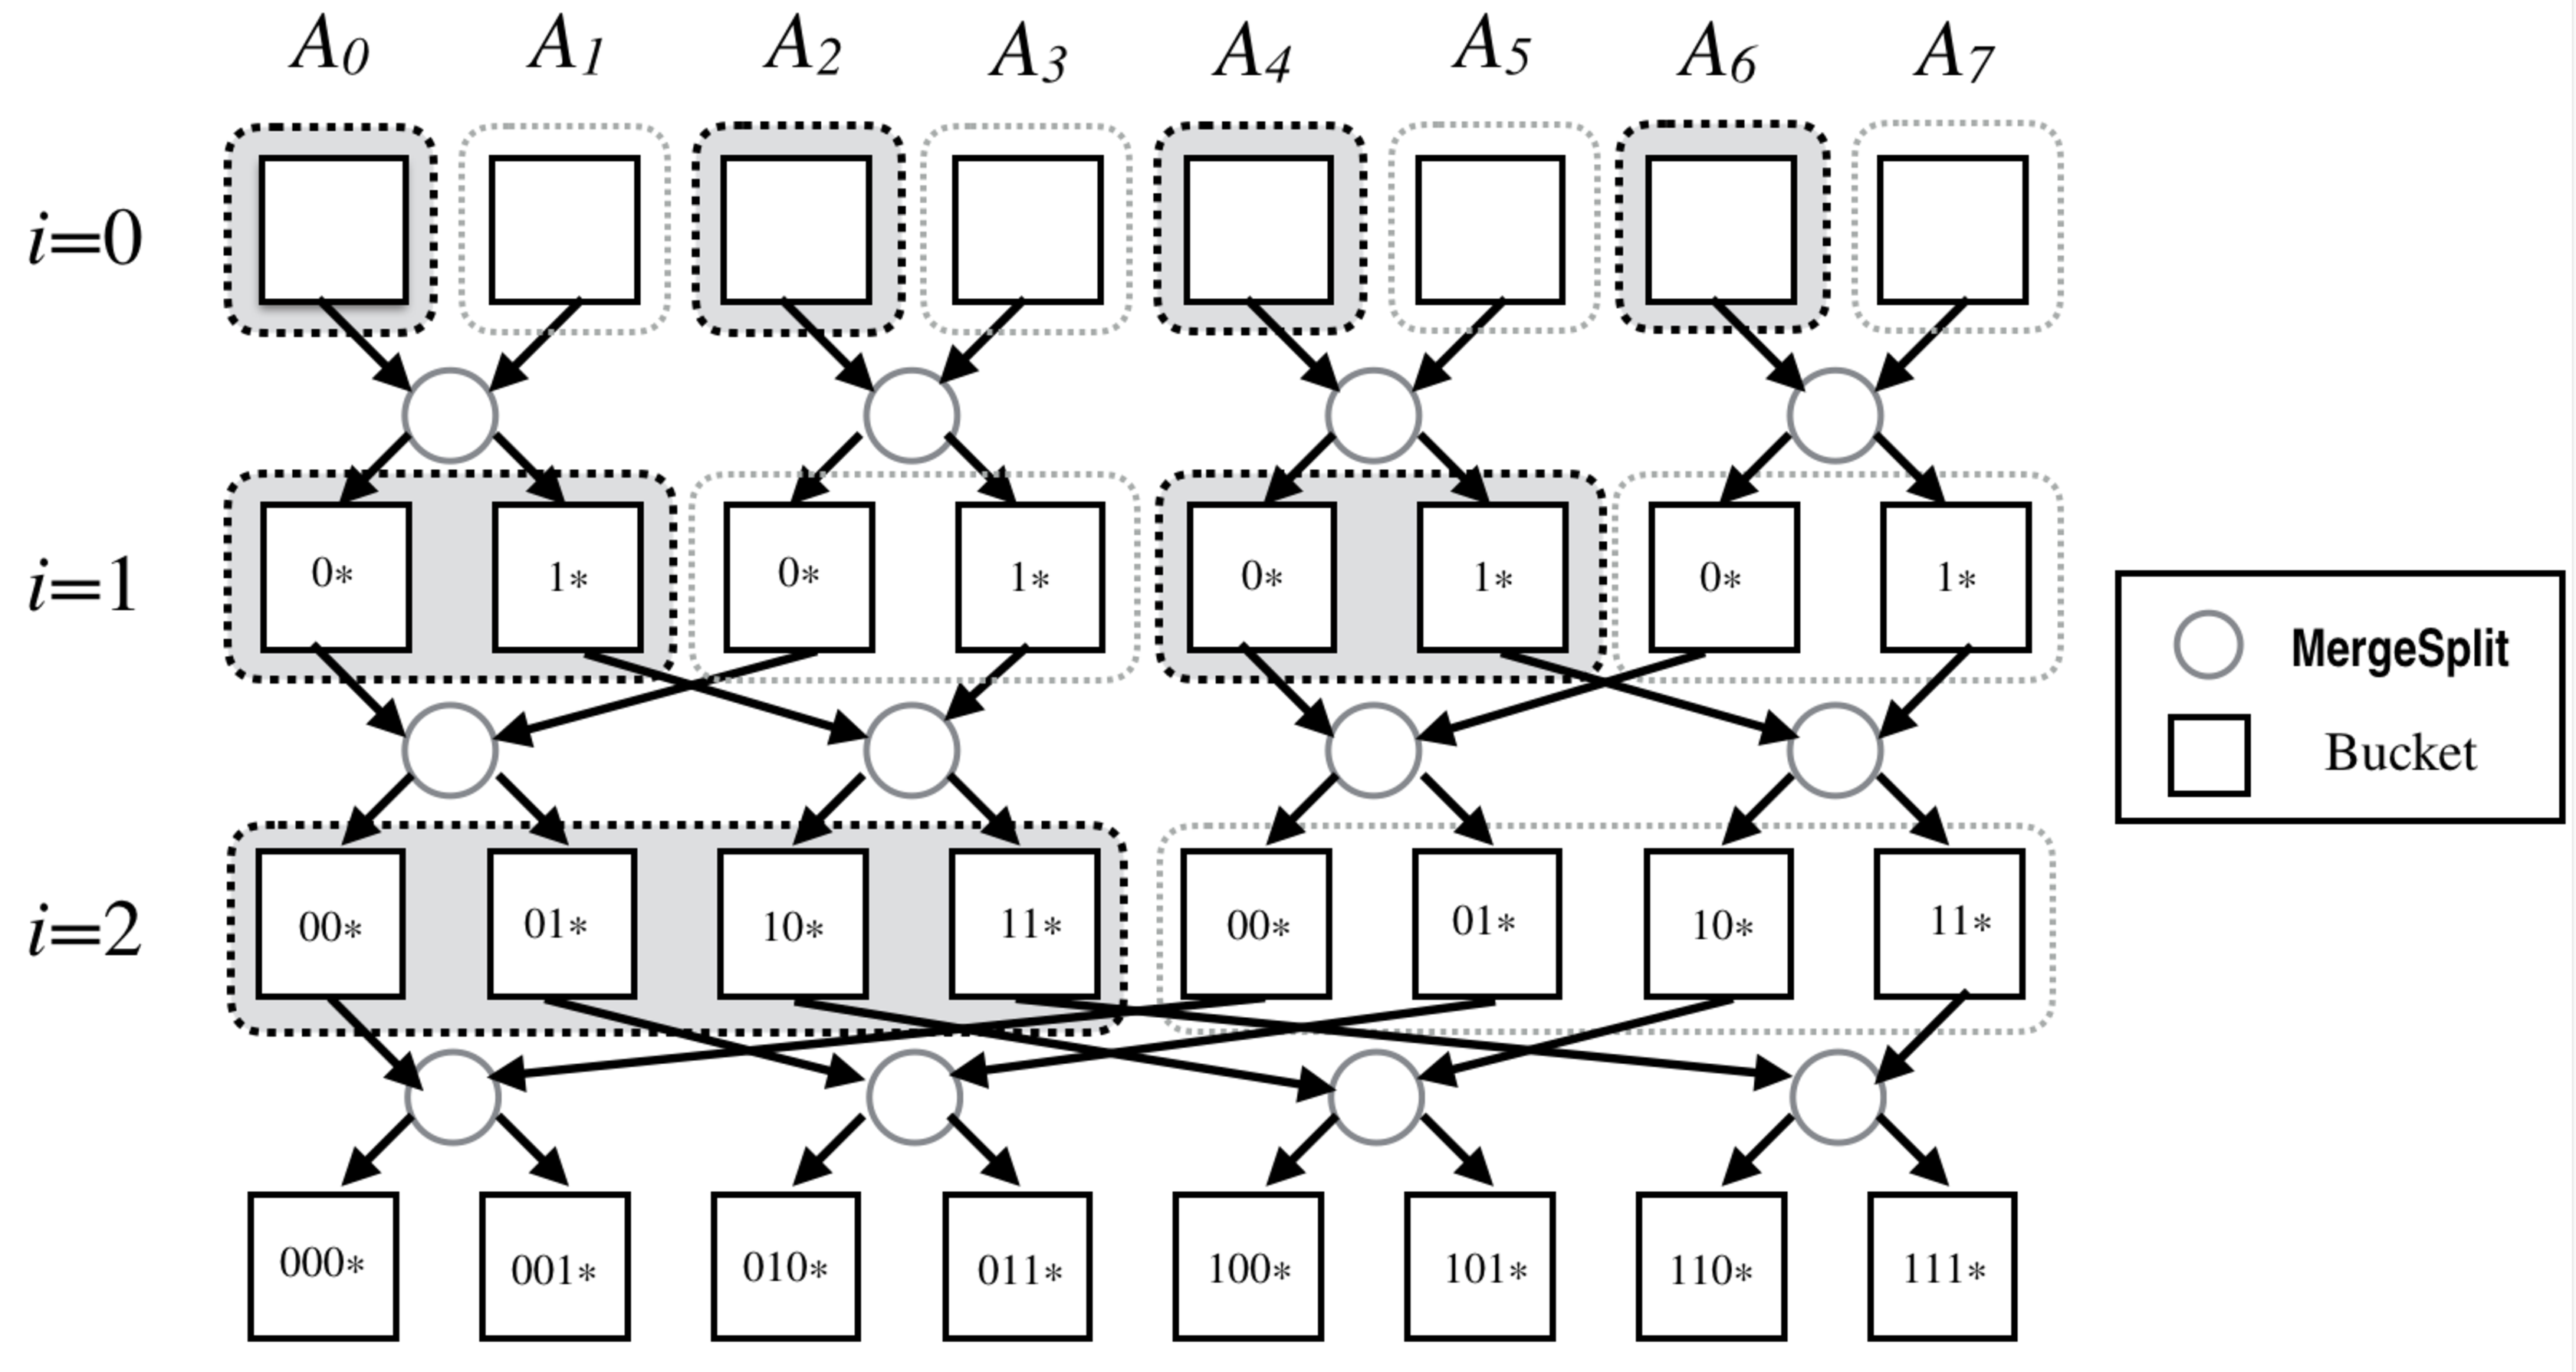
\includegraphics[width=0.7\textwidth]{RadixBucketSort1.pdf}
\captionof{figure}{\textbf{Oblivious random bin assignment with 8 buckets.}
The \textsc{MergeSplit} procedure takes elements from two buckets at level $i$ and put them into two buckets at level $i+1$, according to the $(i+1)$-th most significant bit of the keys. 
At level $i$, every $2^{i}$ consecutive buckets are semi-sorted by the most significant $i$ bits of the keys.}
\label{fig:radix-sort}

%\begin{table*}[t]
\bigskip
\centering
\begin{tabular}{|c|c|c|c|c|}
    \hline
    Algorithm & Oblivious & Client storage & Runtime & Error probability \\
    \hline
    Merge sort & No & $O(1)$ & $2n \log n$ & 0 \\
    Bitonic sort & Yes & $O(1)$ & $n\log^2 n$ & 0 \\
    AKS sort~\cite{aks} & Yes & $O(1)$ & $5.4\times10^7 \times n\log n$ & 0 \\
    Zig-zag sort~\cite{zigzag} & Yes & $O(1)$ & $8\times10^4 \times n\log n$ & 0 \\
    Randomized Shellsort~\cite{RandShellsort} & Yes & $O(1)$ & $24n\log n$ & $\approx n^{-3}$ \\
    \hline
    \textbf{Bucket oblivious sort} & Yes & $2Z$ & $6 n\log n$ & $\approx e^{-Z/6}$\\
    \textbf{Bucket oblivious sort} & Yes & $O(1)$ & $\approx 2n\log n \log^2 Z$ & $\approx e^{-Z/6}$ \\
    \hline   
\end{tabular}
\captionof{table}{\textbf{Runtime of bucket oblivious sort and
classic non-oblivious and oblivious sort algorithms.} Bitonic
sort requires $\frac 14 n \log^2 n$ comparisons. The number of comparisons for AKS
sort and zig-zag sort are cited from \cite{zigzag}. Runtime
represents the number of memory accesses, which is four times the
number of comparisons.}
\label{tab:compare}
%\end{table*}

\end{figure*}

The core of our algorithms is to assign each element to a random bin and then route the elements through a butterfly network to their assigned random bins. 
This part is inspired by Bucket ORAM~\cite{fletcher2015bucket}. 
In more detail, we divide the $n$ elements into $B=2n/Z$ buckets of size $Z/2$ each and add $Z/2$ dummy elements to each bucket.
Now, imagine that these $B$ buckets form the inputs of a butterfly network --- for simplicity, assume $B$ is a power of two.
Each element is uniformly randomly assigned to one of the $B$ output buckets, represented by a key of $\log B$ bits.
The elements are then routed through the butterfly network to their respective destinations.
Assuming the client can store two buckets locally at a time, at level $i$, the client simply reads elements from two buckets that are distance $2^i$ away in level $i$ and writes them to two adjacent buckets in level $i+1$, using the $i$-th bit of each element's key to make the routing decision. 
We refer readers to Figure~\ref{fig:radix-sort} for a graphical illustration.

The above algorithm is clearly oblivious, as the order in which the client reads and writes the buckets is fixed and independent of the input array. If no bucket overflows, all elements reach their assigned destinations. By setting $Z$ appropriately, we can bound the overflow probability.

Our bucket oblivious sort and bucket ORP algorithms are derived from
the above oblivious random bin assignment building block. 

\paragraph{From oblivious random bin assignment to ORP and oblivious sort.}
To obtain a random permutation, we simply remove all dummy elements and randomly permute 
each bucket of the final layer.
Since the client can hold $Z$ elements, permuting each bucket can be done locally. 
We show that the algorithm is oblivious and gives a random permutation despite revealing the number of dummy elements in each destination bucket.
To get oblivious sort, we can first perform ORP on the input array then apply any \emph{non-oblivious, comparison-based} sorting algorithm (e.g., quick sort or
merge sort). We show that the composition of ORP and non-oblivious sort results in an oblivious sort. 

\paragraph{Dealing with small client storage.}
In Section~\ref{sec:O1client}, we extend our algorithms to support $O(1)$ client storage. 
We can rely on bitonic sort to realize the \textsc{MergeSplit} operation that operates on 4 buckets at a time,
which would result in $O(n\log n\cdot \log^2 Z)$ runtime. 

\paragraph{Locality.} Algorithmic performance when the data is stored on disk has been studied in the external disk model (e.g.,~\cite{RuemmlerW94,ArgeFGV97,Vitter01,Vitter06}) and references within). Recently, Asharov et al.~\cite{AsharovCNPRS19} extended this study to oblivious algorithms.  We discuss how our algorithms can be made locality-friendly in Section~\ref{sec:locality}. 


%\paragraph{Organization.}
%The rest of the paper is organized as follows. Our algorithms are simple and intuitive. The access pattern of all our algorithms is deterministic, and therefore security is trivial and all we have to prove is correctness. In Section~\ref{sec:construction} we give our construction and in Section~\ref{sec:extensions} we describe simple extensions. In Appendix~\ref{sec:defs}  define the RAM model of computation and obliviousness. In Appendix~\ref{appx:formal} we give all omitted proofs. 

%
%
%\paragraph{From oblivious bin assignment to ORP.}
%To obtain a random permutation, a simple approach is to remove the dummy elements and permute within each bucket of the final layer. Since the client can hold $Z$ elements, permuting each bucket obliviously can be done locally. 
%
%
%Our bucket oblivious sort and bucket ORP build on top of the above oblivious random bin assignment. 
%To get ORP, simply remove all dummy elements, randomly permute each bucket of the final level, and concatenate the bins.
%To sort, we can simply apply any non-oblivious comparison-based sort (e.g., merge sort) on the randomly permuted elements. 
%
%In Section~\ref{sec:O1client}, we will discuss how to extend our algorithms to support constant client storage
%We can rely on Bitonic sort to realize the ${\bf MergeSplit}$ operation, which would result in $\approx 2n\log n \log^2 Z$ runtime.
%Recently, Asharov et al.~\cite{AsharovCNPRS19} initiate the study of data locality on oblivious algorithms. 
%We observe that our algorithms are be made locality-friendly, and refer readers to Appendix~\ref{sec:locality} for the exact definitions and complexity measures.

%%% Local Variables:
%%% mode: latex
%%% TeX-master: "main"
%%% End:

%!TEX root = main.tex

\newcommand{\memsize}{{N}}
\newcommand{\blocksize}{{b}}
%\newcommand{\negl}{{\sf negl}}
\newcommand{\Y}{{\bf Y}}

%\section*{Appendix}
%In the following we formally define the RAM model of computation, and formally prove obliviousness of our algorithms. 
%
\section{Preliminaries}
\label{sec:defs}

\paragraph{Notations and conventions.}
Let $[n]$ denote the set $\{1,\ldots,n\}$. Throughout this paper, we will use
$n$ to denote the size of the instance and use $\lambda$ to denote the security parameter. 
%A function $\negl$ is called \emph{negligible} if for any constant $c > 0$ and all sufficiently large $\sec$'s, it holds that $\negl < \sec^{-c}$. 
For an ensemble of distributions $\{D_\sec\}$ (parametrized with $\sec$),
we denote by $x \leftarrow D_\sec$ a sampling of an instance from the distribution $D_\sec$. 
We say two ensembles of distributions $\{X_\sec\}$~and~$\{Y_\sec\}$ 
are $\e(\sec)$-statistically-indistinguishable, denoted $\{X_\sec\} \overset{\e(\sec)}{\equiv} \{Y_\sec\}$, 
if for any unbounded adversary $\A$, 
\[
\left|\Pr_{x\leftarrow X_\sec}\left[\A(1^\lambda, x)=1\right] - \Pr_{y\leftarrow Y_\sec}\left[\A(1^\lambda, y)=1\right] \right| \leq \e(\sec) \ .
\]


%For simplicity, we will omit writing the unary security parameter input $1^\lambda$ to all procedures.
%\rl{We are writing the unary security parameter at a lot of places now. Should we add it everywhere and remove this statement?}
% Also, \emph{work} (or bandwidth) is always specified in terms of number of blocks of size $\Omega(\log N)$ accessed.

%\subsection{Memory with Multiple Disks and Data Locality}
%\label{sec:modeling-locality-formal}
%%\paragraph{Random-access machines.}
%%A RAM is an interactive Turing machine that consists of a memory and a CPU.  The
%%memory is denoted as $\mem[N,\bsize]$, and is indexed by the logical
%%address space $[N] = \{1,2,\ldots,N\}$. We refer to each memory word also as a
%%\emph{block} and we use $\bsize$ to denote the bit-length of each block. The CPU
%%has an internal state that consists of $O(1)$ words. The memory supports read/write
%%instructions $(\op,\addr, \data)$, where $\op \in \{\Read,\Write\}$, $\addr \in
%%[N]$ and $\data \in \bit^\bsize \cup \{\bot\}$.  If $\op = \Read$, then
%%$\data=\bot$ and the returned value is the content of the block located in
%%logical address $\addr$ in the memory. If $\op=\Write$, then the memory data in
%%logical address $\addr$ is updated to $\data$.
%%
%%
%%\paragraph{Locality.}
%%We model locality by dividing the memory address space $[N]$ to $\disks$ disks, simply by dividing the memory space to $\disks$ 
%
%
%% \kartik{define bandwidth?}
%To understand the notion of data locality, it may be convenient
%to view the memory as $\disks$ rotational hard drives or other
%storage mediums where sequential accesses are faster than random
%accesses. The program interacting with the memory has to specify
%which disk to access.  
%Each disk is equipped with one read/write head. In order to serve
%a $\Read$ or $\Write$ request with address $\addr$ in some disk
%$\disk \in [\disks]$, the memory has to move the read/write head
%of the disk $\disk$ to the physical location $\addr$ to perform
%the operation.  
%Any such movement of the head introduces cost and delays,  
%and the machine that interacts with the memory would like to
%minimize the  number of move head operations. 
%Traditionally, the latter can be improved by 
%ensuring that the program accesses contiguous regions of the
%memory. 
%% storing related
%% items to physically proximate areas on the memory.  
%However, this poses a great challenge for oblivious computation
%in which data is often continuously shuffled across memory.  
%
%More formally, a memory is denoted as $\mem[N,\bsize,\disks]$,
%consisting of $\disks$ disks, indexed by the address space $[N] =
%\{1,2,\ldots,N\}$, where $\disks \cdot N$ is the size of the
%logical memory. We refer to each memory word also as a
%\emph{block} and we use $\bsize$ to denote the bit-length of each
%block.  
%The memory supports the following two types of instructions.
%\begin{MyItemize}
%\item {\bf \boldmath Move head operation} $(\move,\disk,\addr)$
%moves the head of the $\disk$-th disk ($\disk \in [\disks]$) to point to address $\addr$ within that disk. 
%
%\item {\bf \boldmath A read/write operation} $(\op,\disk,\data)$, 
%where $\op \in \{\Read,\Write\}$, $\disk \in [\disks]$ and $\data \in \bit^\bsize \cup \{\bot\}$. 
%If $\op = \Read$, then $\data=\bot$ and $\mem$ should return the content of the block pointed to by the $\disk$-th disk; 
%If $\op=\Write$, the block pointed to by the $\disk$-th disk is updated to $\data$. The $\disk$-th head is then incremented to point to the next consecutive address, and wrapped around when the end of the disk is reached. 
%
%\end{MyItemize}
%
%\medskip
%\noindent
%{\bf Locality.}
%%\paragraph{Locality.}
%% The number of $\move$ operations defines locality.
%A sequence of memory operations has $(\disks,
%\locparam)$-locality if it contains $\locparam$ $\move$
%operations to a memory that is equipped with $\disks$ disks.  
%
%
%\medskip
%\noindent
%{\bf Relation to the standard memory definition.}
%%\paragraph{Relation to the standard memory definition.} 
%Instead of specifying which disk to read from/write to, we can define a memory of range $[\disks\cdot N] = \{1,\ldots,\disks\cdot N\}$. 
%The address space determines the disk index, and therefore also
%whether or not to move the read/write head. Thus, one can
%consider the regular notion of a RAM program, and our definition
%provides a way to measure the locality of the program. Different implementations
%of the same  functionality can have different locality, similarly to other metrics.

\paragraph{Random-access machines.}
A RAM is an interactive Turing machine that consists of a memory and a CPU.  The
memory is denoted as $\mem[\memsize,\blocksize]$, and is indexed by the logical
address space $[N] = \{1,2,\ldots,N\}$. We refer to each memory word also as a
\emph{block} and we use $\bsize$ to denote the bit-length of each block. The memory supports read/write
instructions $(\op,\addr, \data)$, where $\op \in \{\Read,\Write\}$, $\addr \in
[N]$ and $\data \in \bit^\bsize \cup \{\bot\}$.  If $\op = \Read$, then
$\data=\bot$ and the returned value is the content of the block located in
logical address $\addr$ in the memory. If $\op=\Write$, then the memory data in
logical address $\addr$ is updated to $\data$.
We use standard setting that $\blocksize = \Theta(\log N)$ (so a word can 
store an address).
%We follow the convention that the CPU performs one \emph{word-level operation} per unit time,
%i.e., arithmetic operations (addition or subtraction), 
%bitwise operations (AND, OR, NOT, or shift), memory accesses (read or write), or
%evaluating a pseudorandom function~\cite{oram00,oram09,oram03,oblivhash,LarsenN18,panorama}.

\medskip
\noindent
{\bf Obliviousness.}
Intuitively, a RAM program $M$ obliviously simulates a RAM program $f$ if: (1) it has the same input/output behavior as $f$; (2) There exists a simulator $\Sim(\abs{x})$ that produces access pattern that is statistically close to the access pattern of $M(x)$, i.e., it can simulate all memory addresses accessed by $M$ during the execution on $x$, without knowing $x$. In case the access pattern and the functionality are randomized, we have to consider the joint distribution of the simulator and the output of the RAM program or the functionality. 

%In our sorting algorithm, the access pattern is randomized but the functionality is deterministic. In the oblivious random permutation algorithm, the access pattern is deterministic but the functionality is randomized. As always either the access pattern or the functionality is deterministic, we can consider a simpler definition of obliviousness in which the functionality and the simulation are considered separately. 

For a  RAM machine $M$ and input $x$, let ${\sf AccPtrn}(M(x))$ denote the distribution of memory addresses a machine $M$ produces on an input $x$.
\begin{definition}
A RAM algorithm $M$ obliviously implements the functionality $f$ with $\e$-obliviousness if the following hold:
\begin{eqnarray*}
\left\{\Sim(1^\lambda),f(x)\right\}_{x \in \bit^\lambda} \overset{\epsilon(\lambda)}{\equiv} \left\{ {\sf AccPtrn}(M(x)),M(x)\right\}_{x \in \bit^\lambda}
\end{eqnarray*}
If $\epsilon(\cdot)=0$, we say $M$ is perfectly oblivious. 
%\[ \left\{\Sim(1^\lambda),f(x)\right\}_{x \in \bit^\lambda} 
%\overset{\epsilon(\lambda)}{\equiv} \left\{ {\sf AccPtrn}(M(x)),M(x)\right\}_{x \in \bit^\lambda} \]
\end{definition}

%$$
%$$
%\begin{MyItemize}
%
%\item {\bf $\delta$-Correctness:} For every input $x$ it holds that 
%$$
%\Pr\left[M(x) = f(x) \right] \geq 1- \delta(\abs{x})
%$$
%
%\item {\bf $\e$-Obliviousness:} There exists a simulator $\Sim(\abs{x})$ such that
%$$
%\left\{{\sf AccPtrn}(M(x))\right\}_{\abs{x}} \overset{\e(\abs{x})}{\equiv} 
%\left\{\Sim(\abs{x})\right\}_{\abs{x}}
%$$
%%that produces access pattern that is statistically close to the access pattern of $M(x)$.
%\end{MyItemize}
%\end{definition}

%A functionality $f$ is a (possibly randomized) RAM machine that gets some input $x$ and computes an output $y$. A RAM algorithm $M$ obliviously implements the functionality $f$ if: (1) it has the same input/output behavior as $f$; (2) There exists a simulator $\Sim(\abs{x})$ that produces access pattern that is statistically close to the access pattern of $M(x)$. I.e., it can simulates all memory addresses accessed by $M$ during the execution on $x$, without knowing $x$. Note that all our algorithms have deterministic access pattern, and therefore 
%
%In case where the functionality $f$ is randomized, we require that the joint distribution of the output of the functionality and the output of the simulator would be statistically close to the output of the algorithm $M$ and its access pattern. Formally, we let ${\sf AccPtrn}(M(x))$ denote the distribution of memory addresses a machine $M$ produces on an input $x$. We have:
%
%\begin{definition}[Oblivious machines]
%\label{defn:omachine}
%Let $f,M:\bit^* \rightarrow \bit^*$ be (possibly randomized) RAM programs. We say that $M$ {\em obliviously simulates $f$} if there exists a  simulator $\Sim$ and a negligible function $\epsilon(\cdot)$ such that  for any $\lambda$:% and any input $x$ of size $\lambda$ it holds that:
%\begin{eqnarray*}
%\hspace{-5ex}\lefteqn{\left\{\Sim(1^\lambda),f(x)\right\}_{x \in \bit^\lambda}} \\
%&&\hspace{+5ex}\overset{\epsilon(\lambda)}{\equiv} \left\{ {\sf AccPtrn}(M(x)),M(x)\right\}_{x \in \bit^\lambda}
%\end{eqnarray*}
%If $\epsilon(\cdot)=0$, we say $M$ is perfectly oblivious. 
%\end{definition}

The two main functionalities that we focus on in this paper are the following:

\paragraph{Oblivious sort:}
This is a deterministic functionality in which the input is an array $A[1,\ldots,n]$ of memory blocks (i.e., each $A[i] \in \bit^\blocksize$, representing a key). The goal is to output an array $A'[1,\ldots,n]$ which is some permutation $\pi:[n] \rightarrow [n]$ of the array $A$, i.e., $A'[i] = A[\pi(i)]$, such that $A'[1]\leq \ldots \leq A'[n]$. %Obliviousness is defined using Definition~\ref{defn:omachine}. We denote this functionality as ${\cal F}_{\rm sort}$. 

\paragraph{Oblivious permutation:} 
This is a randomized functionality in which the input is an array $A[1,\ldots,n]$ of memory blocks. The functionality chooses a random permutation $\pi:[n] \rightarrow [n]$ and outputs an array $A'[1,\ldots,n]$ such that $A'[i] = A[\pi(i)]$ for every $i$. %Obliviousness is defined using %Definition~\ref{defn:omachine}. Note that the definition requires that the access pattern does not leak the permutation chosen by the functionality. We denote this functionality ${\cal F}_{\rm perm}$. 
%\end{MyItemize}


%\section{Obliviousness}
%\label{appx:formal}
%In this section we provide proofs for obliviousness of our constructions. In Section~\ref{sec:rand:functionality} we formally define the ideal functionality of the random bin assignment (Algorithm~\ref{code:obin}). 
%
%
%\subsection{\boldmath Random Bin Assignment: Functionality}
%\label{sec:rand:functionality}
%We start with defining the oblivious random bin assignment functionality, which we denote by $f_{\rm randbin}$. In a nutshell, given some input array ${\bf X}$ we consider an output array which has twice the size of the input array, and we consider the output array as $B$ consecutive bins. We assign each ``real'' element of the input array into a random bin in the output array, and pad each bin with dummy elements. We will show how to realize the functionality for $Z := \alpha \log \lambda$ with $\alpha \in \omega(1)$ and $\lambda$ is the security parameter. 
%
%
%\begin{myfunc}
%[\boldmath ${\cal F}_{\rm randbin}(\X,Z)$]
%\label{func:bin-assignment}
%The random bin assignment functionality ${\cal F}_{\rm randbin}(\X,Z)$ is defined as follows:
%\begin{MyItemize}
%\item {\bf Input:} an input an array $\X$ of length $n$ containing real and dummy elements, and a bin size~$Z$. 
%\item {\bf The functionality:} 
%\begin{MyEnumerate}
%\item Define an output array $\Y$ of size $2n$, containing $B = 2n/Z$ bins of size $Z$ each, denoted as $\Y_1,\ldots,\Y_B$. 
%\item For every real element in $\X$ choose a random destination bin $i \gets [B]$, and place the element in the $i$th output bin. 
%\item If some output bin contains more than $Z$ elements, then {\sf abort}. 
%\item Pad each output bin to its maximal capacity using dummy elements. Order each output bin as follows: 
%(1) all real elements appear before dummies;
%and (2) real elements are ordered according to their ordering (indices) in the input array $\X$.
%\end{MyEnumerate}
%\end{MyItemize}
%\end{myfunc}
%
%
%\begin{lemma}
%Let $Z = \alpha \log \lambda$ for any super-constant function $\alpha(\lambda)$.
%Algorithm~\ref{code:obin}
%obliviously simulates ${\cal F}_{\rm randbin}$ (i.e., Functionality~\ref{func:bin-assignment}) with $\epsilon(n, Z) = 2n/Z \cdot \log(2n/Z) \cdot e^{-Z/6}$ failure probability. %The algorithm completes in $O(\frac{n}{Z}\log n \cdot T_{\sf MergeSplit}(Z))$ work, where $T_{\sf MergeSplit}(Z)$ .
%\label{lem:randbin}
%\end{lemma}
%\begin{proof}
%The access pattern of Algorithm~\ref{code:obin} is deterministic and is independent of the input, and therefore it can be simulated easily. Moreover, since it is deterministic, it suffices to consider correctness and access pattern separately, and there is no need to consider the joint distribution. 
%As for correctness, we claim that the algorithm implements Functionality~\ref{func:bin-assignment}. Specifically, the functionality and the algorithm choose the same bin assignment for all elements with the exact same probability. Moreover, for the same bin assignments for all elements, the functionality and the algorithm result in the same output, except for a negligible probability of failure. This occurs when there is some internal overflow in the algorithm in one of the iterations $i \in \{1,\ldots,\log B\}$, which does not occur in the functionality. 
%%As for efficiency, we run ${\sf MergeSplit}$ exactly $B \log B$ times, which results in $O(\frac{n}{Z}\log n \cdot T_{\sf MergeSplit}(Z))$. 
%%	%Sorting each bin results in $B \cdot (Z \log^2 Z) = n \log^2 Z$, which is smaller than $O(n \log n)$. 
%\end{proof}
%%
%%\subsection{Oblivious Sort from Oblivious Random Bin Assignment}
%%\label{sec:obliviousSortFromRandomBinAssignment}
%%
%%We formalize the composition theorem: Given an oblivious random bin assignment, 
%%%\paragraph{Oblivious sort from random bin assignment algorithm  and non-oblivious sort.}
%%Given a random bin assignment algorithm 
%%${\sf ObliviousRandomBin}$ and a non-oblivious
%%comparison-based sorting algorithm ${\sf NonObliviousSort}$ (e.g., Merge-Sort), one can 
%%easily construct
%%an oblivious sorting algorithm as follows. 
%%%
%%\begin{myalgorithm}
%%[${\sf ObliviousSortFromRandomBinAssignment}(\X)$]
%%\label{alg:sort-from-random-bin}
%%\leavevmode
%%\begin{MyEnumerate}%[leftmargin=5mm]
%%\item 
%%Given an input array $\X$, invoke the random bin assignment algorithm to receive $\Y: = {\sf ObliviousRandomBin}(\X)$. Note that in each ``bin'' of $\Y$, the real elements appear before the dummy elements, and are sorted. Moreover, $\abs{\Y}=2\abs{\X}$.  
%%
%%%\item Obliviously sort each bucket $A_0,\ldots,A_{B-1}$ using Bitonic Sort, sorting the real elements according to their keys, and preferring real elements over dummy elements. 
%%
%%
%%\item Sort $\Y$ using a (non-oblivious) comparison-based sorting algorithm. 
%%That is, invoke ${\Y'} := {\sf NonObliviousSort}(\Y)$, while preferring real elements over dummy elements. 
%%Formally speaking, a sorting algorithm is comparison-based if the physical access pattern depends only on the relative ranking of elements in the input. 
%%A technical condition we need is that no two elements have the same rank. This can be ensured by resolving any tie consistently by the initial location of the elements in the array $\Y$.
%%
%%\item Now, all dummy elements appear at the $n$ last locations of $\Y'$. Truncate the last $n$ elements of $\Y'$. 
%%
%%\end{MyEnumerate}
%%\end{myalgorithm}
%%
%%%Let ${\sf Truncate}$ denote the last step of the above algorithm. Then, our sorting algorithm can be described as the following simple composition 
%%%$$ {\sf Truncate}({\sf NonObliviousSort}({\sf ObliviousRandomBin}(\X))) \ .$$
%%
%%\paragraph{Why is it oblivious?} 
%%Given that we do not fully permute the input array, a natural question is why the above composition is still oblivious. Essentially, the composition still holds since there is a 1-to-1 mapping between any input of the array and every possible output of the ${\cal F}_{\rm randbin}$ functionality, i.e., every possible input of the non-oblivious sorting algorithm. This mapping is exactly the random assignment of the destination bins. Therefore,  every access pattern in the non-oblivious sorting part of the algorithm, can be justified with some specific random assignment on the input array, for every possible ordering of the input array. However, some of the  assignments are ``invalid'' due to overflows; yet, overflows occur with negligible probability, and therefore we get statistical security. We proceed to the formal proof of security:
%%
%%\begin{lemma}[From oblivious random bin to oblivious sort]
%%Suppose that {\sf ObliviousRandomBin} is a statistically (or perfectly resp.)
%%oblivious random bin assignment algorithm.
%%Then, 
%%the above algorithm is a statistically (or perfectly resp.) secure 
%%oblivious sorting algorithm. 
%%\label{lem:orpsort}
%%\end{lemma}
%%\begin{proof}
%%Since the functionality is deterministic, we can consider obliviousness and correctness separately. Correctness of the algorithm is trivial. 
%%We next prove the obliviousness of the algorithm. 
%%We prove for the case of perfect security, since statistical security is similar,
%%except that we replace ``identically distributed'' with ``statistically close''.
%%
%%
%%Let ${\sf SimRandBin}$ be the simulator algorithm for 
%%the underlying oblivious random bin assignment.
%%Consider any given input $\X$ of length $n$, 
%%and let $(\Y, {\sf addressesRandBin})$ 
%%denote the joint distribution of the outcome array $\Y$ and the addresses
%%accessed during an execution of the oblivious random bin assignment.
%%Lemma~\ref{lem:randbin} implies that:
%%$$
%%\left(\Y, {\sf addressesRandBin}\right) \equiv \left({f}_{\rm randbin}(\X), {\sf SimRandBin}(1^n,|\X|)\right)  \ . \vspace{-1ex}
%%$$
%%Let ${\sf SortAddresses}(\Y)$ 
%%denote the addresses observed during an execution 
%%of the truncation algorithm and the non-oblivious, comparison-based 
%%sorting algorithm upon receiving input array $\Y$.
%%We thus have that\vspace{-1ex}
%%\begin{eqnarray*}
%%\hspace{-15ex}\lefteqn{\left({\sf SortAddresses}(\Y), {\sf addressesRandBin}\right)}\\
%%&& \hspace{+15ex}\equiv 
%%\left({\sf SortAddresses}({f}_{\rm randbin}(\X)), {\sf SimRandBin}(1^n,|\X|)\right) \ .   \vspace{-1ex}
%%\end{eqnarray*}
%%For any comparison-based 
%%sort, its access patterns depend only on 
%%the relative ranking of the input elements. Since without loss of generality, 
%%we assumed that the input array $\X$ always has distinct values, and we carefully defined how to avoid any ties, 
%%we have that\vspace{-1ex}
%%$$
%%{\sf SortAddresses}({f}_{\rm randbin}(\X)) \equiv
%%{\sf SortAddresses}({f}_{\rm randbin}([|\X|])) \ , \vspace{-1ex}
%%$$
%%where $[|\X|] = \{1,\ldots,|\X|\}$. 
%%Now, 
%%observe that we can construct a simulator 
%%${\sf SimObliviousSort}$
%%that simply outputs 
%%$$
%%{\sf SortAddresses}({f}_{\rm randbin}([|\X|])), {\sf SimRandBin}(1^n,|\X|)
%%$$
%%This simulator's output is identically distributed
%%as the real-world access patterns of executing
%%the aforementioned sorting algorithm, i.e., to $({\sf SortAddresses}(\Y), \allowbreak{\sf addressesRandBin})$. 
%%\end{proof}
%%
%%%We therefore conclude:
%%%\begin{corollary}
%%%\label{cor:rand-bin-using-bitonic}
%%%Let $Z = \alpha \log \lambda$ for any super-constant function $\alpha(\lambda)$, and assume that a client can store $4\cdot Z$ elements locally. 
%%%Algorithm~\ref{alg:bucket-sort}, where ${\sf MergeSplit}$ 
%%%obliviously simulates ${\cal F}_{\rm randbin}$ (i.e., Functionality~\ref{func:bin-assignment}) with $\negl$ statistical 
%%%failure. The algorithm completes in $O(n \log n)$ work.
%%%\end{corollary}
%%
%%%\medskip
%%%\noindent
%%%{\bf Building blocks.} Moreover, in Appendix~\ref{sec:building-blocks} we review some building blocks that we will use in our construction, including oblivious sorts, {\sf Dedup} -- an algorithm that removes duplicates obliviously based on oblivious sorts, and Oblivious Bin Packing -- an algorithm that receives an array as an input, where each element is marked with some destination bin, and the algorithm obliviously routes the elements into the bin, while padding each bin to its maximal capacity with dummy elements. This is again implemented using oblivious sorts. See Appendix~\ref{sec:building-blocks} for further details.   
%%
%%%%% Local Variables:
%%%%% mode: latex
%%%%% TeX-master: "main"
%%%%% End:

%!TEX root = main.tex




\section{Our Construction} 
\label{sec:construction}
\label{sec:random-bin-assignment}

We first present the oblivious random bin assignment algorithm (Section~\ref{sec:obin})  and then use it to implement our bucket oblivious random permutation (Section~\ref{sec:ORP}) and bucket oblivious sort (Section~\ref{sec:osort}).

\newcommand{\val}{{\sf value}}
\newcommand{\pref}{{\sf pref}}

\input{code}
\subsection{Oblivious Random Bin Assignment.}
\label{sec:obin}

The input to the oblivious random bin assignment algorithm is an array $\X$ of $n$ elements. 
The goal is to obliviously and uniformly randomly distribute the elements into a set of bins. Each element is assigned to independent random bin, and elements are then routed into the bins obliviously. 

The algorithm first chooses a bucket size $Z$, which can be set to the security parameter $\sec$. 
Then, it constructs $B=\lceil 2n/Z \rceil$ buckets each of size $Z$.
Without loss of generality, assume $B$ is a power of $2$ --- if not, pad it to the next power of 2. Note that the algorithm introduces $n$ dummy elements, and the output is twice the size of the input array. %If needed, see Appendix~\ref{appx:formal} for a formal definition of the functionality. 

%also assume elements in $\X$ are distinct --- if not, we can use the indices of the elements within $\X$ to break ties.

Figure~\ref{fig:radix-sort} gives a graphic illustration of the algorithm for 8 input buckets and Algorithm~\ref{code:obin} gives the pseudocode.
Each element in $\X$ is assigned a random key in $[0, B-1]$ which represents a destination bucket.
Next, the algorithm repeatedly calls the \textsc{MergeSplit} subroutine to exchange elements between bucket pairs in $\log B$ levels to distribute elements into their destination buckets. 
The operation $(A'_0,A'_1)\leftarrow \textsc{MergeSplit}(A_0,A_1,i)$ involves four buckets at the time, distributing the elements in the two input buckets $A_0$ and $A_1$ into two output buckets $A'_0$ and $A'_1$.
$A'_0$ receives all the keys with $(i+1)$-th most significant bit (MSB) as 0 and $A'_1$ receives all the keys with $(i+1)$-th MSB as 1.


For now, assume the client can locally store two buckets.
For each \textsc{MergeSplit}, it reads (and decrypts) the two input buckets, swaps elements in the two buckets according to the above rule, and writes to the two output buckets (after re-encryption).
It is then easy to see that Algorithm~\ref{code:obin} is oblivious since the order in which the client reads and writes the buckets is fixed and independent of the input array.
%We discuss how to extend the algorithm to work with $O(1)$ client storage in Section~\ref{sec:O1client}. 

When no bucket overflows, all real elements are correctly put into their assigned bins.
We now show that the probability of overflow is exponentially small in $Z$. 
Intuitively, this is because each bucket contains (in expectation) half dummy elements that serve as a form of ``slack'' to disallow overflow.

\begin{lemma}
\label{lemma:shuffle}
Overflow happens with at most $\epsilon(n, Z) = 2n/Z \cdot \log(2n/Z) \cdot e^{-Z/6}$ probability.
\end{lemma}
\begin{proof}
\label{clm:proof-shuffle}
Consider a bucket $A^{(i)}_b$ at level $i$.
%Let $T$ be the set of real elements. For $t \in T$, $i \in \{1,\ldots,\log B\}$ and $b \in [B]$, let $X_{i,b}^{t}$ be the indicator random variable that $t$ is assigned to bucket $A^{(i)}_b$.
%$X_{i,b}=\sum_{t \in T}X_{i,b}^{t}$ denotes the load of $A^{(i)}_b$. 
Observe that this bucket can receive real elements from $2^i$ initial buckets, each containing $Z/2$ real elements.
For each such element, we have chosen an independent and uniformly random key;
the element reaches $A^{(i)}_b$ only when the most significant $i$ bits of its key match $b$,
which happens with exactly $2^{-i}$ probability.
A Chernoff bound shows that $A^{(i)}_b$ overflows with less than $e^{-Z/6}$ probability.
Hence, a union bound over all levels and all buckets 
shows that overflow happens with less than $B \cdot \log B \cdot e^{-Z/6} = \epsilon(n,Z)$ probability.
\end{proof}

%In Appendix~\ref{appx:formal} we formally describe the ideal functionality of oblivious random bin assignment, and show that the above describe algorithm obliviously implements this functionality. 

\subsection{Bucket Oblivious Random Permutation.}
\label{sec:ORP}

After performing the oblivious random bin assignment, ORP can be simply achieved as follows:
scan the array and delete dummy elements from each bin (note that within each bin it is guaranteed that the real elements appear before the dummy elements). Then obliviously permute each bin and finally concatenate all bins.  We have:

%The ORP reveals the loads of the output buckets of bin assignment, that is, the number of real elements in each bucket. 

\begin{lemma}
Bucket ORP oblivious implement the permutation functionality except for $\e(n,Z)$ probability. 
\end{lemma}

\begin{proof}
We first describe the simulator. 
The access pattern of the oblivious bin assignment algorithm is deterministic and the same for every input, where the overflow even is independent of the input itself. Therefore, it is easy to simulate the bin assignment. 
The simulator then pretends to simulate the randomly permuting of each bin. 
Then, 
the simulator chooses random loads $\vec{k}=(k_0, k_1, \ldots, k_{B-1})$, where $k_i$ is the load of the real elements in the $i$th bin. This is done by simply throwing $n$ elements into $B$ bins (``in the head''). If there is some $i$ for which $k_i > Z$ then the simulator aborts. The removal of the dummy elements is equivalent to the revealing of these loads. 

Clearly, $\vec{k}$ are distributed the same as in the real execution. The only difference between the simulated access pattern and the real one is in the case where the algorithm aborts as a result of an overflow before the last level, which occurs with at most $\e(n,Z)$ probability. 

We next show that the output of the algorithm is a random permutation, conditioned of the access pattern. As we previously described, it is actually enough to condition on the vector of random loads $\vec{k}=(k_0, k_1, \ldots, k_{B-1})$. We show that given any such vector, all permutations are possible.  

Fix a particular load $\vec{k}=(k_0, k_1, \ldots, k_{B-1})$. The algorithm works by first assigning the real elements into the bins, and then permuting within each bin. For every input, there are exactly ${n \choose k_0,\ldots,k_{B-1}}$ ways to distribute the real elements into the bins while achieving the vector of loads $\vec{k}$. Then, each bin is individually permuted, i.e., within each bin $i$, we have $k_i$ different possible ordering. Overall, 
the total number of possible outputs with that load is then
\[{n \choose k_0,\ldots,k_{B-1}} \cdot k_0! \cdot \ldots \cdot k_{B-1}! = n!\]
That is, even conditioned on some specific loads $\vec{k}=(k_0, k_1, \ldots, k_{B-1})$, all permutations are still possible.
Therefore, for every $\pi$, $\Pr\left[\Pi = \pi \mid \vec{K}=\vec{k} \right] = \frac 1 {n!}$, and
\[ \Pr\left[\Pi = \pi\right] = \sum_{\vec{k}} \Pr\left[\Pi = \pi \mid \vec{K}=\vec{k} \right] \cdot \Pr\left[\vec{K}=\vec{k}\right] = \frac {1}{n!} \]
%&= \frac {1}{n!} \cdot \sum_{\vec{k}} \Pr\left[\vec{K}=\vec{k}\right] = \frac {1}{n!}

The ORP fails only when some bin overflows during the oblivious random bin assignment, which happens with $\epsilon(n,Z)$ probability.
\end{proof}

\subsection{Bucket Oblivious Sort.}
\label{sec:osort}
Once we have ORP, it is easy to achieve oblivious sort: just invoke any non-oblivious comparison-based sort after ORP.

Since the functionality is deterministic, it is enough to consider separately correctness and simulation. Correctness follows from directly from the correctness of the ORP and the non-oblivious sort. As for obliviousness, given any input array, one can easily simulate the algorithm by first randomly permuting the array and then running the comparison-based non-oblivious sort. 
The access patterns of a comparison-based sort depend only on the relative ranking of the input elements, which is independent of the input array once the array has been randomly permuted. 

\subsection{Efficiency.}
\label{sec:efficiency}

We analyze the efficiency of our algorithms and compare them to classic non-oblivious oblivious sorting algorithms in Table~\ref{tab:compare}.
We measure runtime using the number of memory accesses the clients needs to perform on the server.



% Merge sort, a well known non-oblivious sort, runs in $2n\log n$ time. 
% It has in $\log n$ stages; each stage merges smaller sorted subarrays into larger sorted subarrays,
% which reads and writes the entire array in the process.
% Bitonic sort uses $\frac 14 n\log^2 n$ comparisons.
% According to~\cite{zigzag}, the AKS sorting network has $13613047 n\log n$ comparisons and the Zigzag sort uses $19600n\log n$ comparisons (with best known explicit constructions). 
% Randomized Shellsort~\cite{RandShellsort} needs $6n\log n$ comparisons (there are $\log n$ iterations, six passes per iteration, and $n$ comparisons per pass). 
% The number of memory accesses is four times of the number of
% comparisons for Bitonic, AKS, Zigzag, and randomized Shellsort.


For our algorithms, assuming the client can store $2Z$ elements locally, each $2n$-sized array is read and written once and there are $\log(2n/Z)<\log n$ of them.
So oblivious bin assignment and bucket ORP run in (less than) $4n\log n$ time.
Note that the last step of ORP, i.e., permuting each output bucket, can be incorporated with the last level of oblivious bin assignment.
Bucket oblivious sort additionally invokes a non-oblivious sort, and thus runs in $6n\log n$ time. 
This is within $3\times$ of merge sort and beats bitonic sort when $n$ is moderately large;
for example, $5\times$ faster than bitonic for $n=2^{30}$.
For an overflow probability of $2^{-80}$ and most reasonable values of $n$, $Z = 512$ suffices. 


%%% Local Variables:
%%% mode: latex
%%% TeX-master: "main"
%%% End:

% !TEX root =  main.tex

\section{Extensions}
\label{sec:extensions}

\subsection{Extension to Constant Client Storage.}
\label{sec:O1client}
We now discuss how to extend our algorithms to the case where the client can only store $O(1)$ elements locally.

Each \textsc{MergeSplit} can be realized with a single invocation of Bitonic sort.
Concretely, we first scan the two input buckets to count how many real elements should go to $A'_0$ vs. $A'_1$, then tag the right number of dummy elements to go to either direction, and finally perform the Bitonic sort.

Next, we need to permute each output bucket obliviously with $O(1)$ local storage. 
This can be done as follows. 
First, assign each element in a bucket a uniformly random label of $\Theta(\log n)$ bits. 
Then, obliviously sort the elements by their random labels using Bitonic sort. 
Since the labels are ``short'' (i.e., logarithmic in size), we may have collisions with $n^{-c}$ probability for some constant $c$, in which case we simply retry. 
In expectation, it succeeds in $1+o(1)$ trials. 

%or use the method in Chan et al.~\cite{opramdepth}[Lemma 10] \rl{what is this?}

Since we invoke $B/2$ instances of Bitonic sort on $2Z$ elements at each level,
the runtime is roughly $\log B \cdot B/2 \cdot 2Z \log^2 (2Z)) \approx 2 n\log n \log^2 Z$. 
%In this case, our ORP and oblivious sort run in approximately $160n\log n$ time. \rl{Not competitive. is this part worth it?}

\subsection{Better Asymptotic Performance.}
Our algorithms can also be extended to have better asymptotic performance.
For this instantiation, we use a primitive called oblivious tight compaction.
Oblivious tight compaction receives $n$ elements each marked as either 0 or 1, and outputs a permutation of the $n$ elements such that all elements marked 0 appear before the elements that are marked 1. 
It should not be hard to see that oblivious tight compaction can be used to achieve \textsc{MergeSplit}.
Using the $O(1)$-client-storage and $O(n)$-time oblivious tight compaction construction from~\cite{asharov2018optorama}, bucket oblivious sort achieves $O(n\log n + n\log^2Z)$ runtime and $O(1)$ client storage.
Setting $Z=\omega(1)\log n$, bucket oblivious sort achieves $O(n\log n)$ runtime, $O(1)$ client storage, and a negligible in $n$ error probability.

\subsection{Locality.}
\label{sec:locality}
Algorithmic performance when the data is stored on disk has been studied in the external disk model (e.g.,~\cite{RuemmlerW94,ArgeFGV97,Vitter01,Vitter06}) and references within). Recently, Asharov et al.~\cite{AsharovCNPRS19} extended this study to oblivious algorithms. In this setting, an algorithm 
is said to have $(p, \ell)$ locality if it has access 
to $p$ disks and 
accesses in total $\ell$ discontiguous memory regions in all disks combined. As an example, it is not hard to see that merge sort is non-oblivious sorting algorithm that sorts an array of size $n$ in $O(n \log n)$ and $(3,\log n)$-locality, whereas quick sort  is not local for any reasonable $p$. 
This locality metric is motivated by the fact that real-world storage
media such as disks support sequential accesses
much faster than random seeks. Thus an algorithm that 
makes mostly sequential accesses would execute much faster in practice than one that  
makes mostly random accesses --- even if the two have the same runtime in a standard
word-RAM model. 

Guided by this new metric, Asharov et al.~\cite{AsharovCNPRS19} consider how to design oblivious algorithms and ORAM schemes that achieve good locality. 
Since sorting is one of the most important
building blocks in the 
design of oblivious algorithms, 
inevitably Asharov et al.~\cite{AsharovCNPRS19}
show a locality-friendly sorting algorithm.
Concretely, they show that there is a specific way to implement
the Bitonic sort meta-algorithm,
such that the entire algorithm requires accessing 
$O(\log^2 n)$ distinct memory regions (i.e., as many as the depth of the sorting network) 
require only 2 disks to be available --- in other words,
the algorithm achieves $(2, O(\log^2 n))$-locality.

We observe that our algorithm, when implemented properly, is a locality-friendly oblivious sorting algorithm. 
Our algorithm 
outperforms Asharov et al.~\cite{AsharovCNPRS19}'s  scheme 
by an almost logarithmic 
factor improvement in locality. % both runtime and locality.
To achieve this, the crux is to implement all $n/Z$ instances of 
$\textsc{MergeSplit}$ in the same layer of the butterfly network 
while accessing a small number of discontiguous regions. Specifically, the $\textsc{MergeSplit}$ operation works on 4 buckets at a time, while reading two buckets from the input layer, and writing to two consecutive buckets in the output layer. Moreover, the different invocations of $\textsc{MergeSplit}$ on the same layer deal with consecutive buckets. By carefully distributing the buckets among the different disks, and by using Bitonic sort while implementing the $\textsc{MergeSplit}$ operation, we conclude:

\begin{corollary}
There exists a statistically oblivious sort algorithm which, except with $\approx e^{-Z/6}$ probability, completes in $O(n \log n \log^2 Z)$ work and with $(3, O(\log n \log^2 Z)$) locality.
\end{corollary}
%
%We observe that our algorithms, when implemented properly, have good data locality.
%The crux is to perform all $n/Z$ instances of 
%$\textsc{MergeSplit}$ in the same level of the butterfly network concurrently.
%We discuss this part in detail in Appendix~\ref{sec:locality}. 


%\medskip
%{\small
%\noindent
%{\bf Disclaimer.}
%This paper was prepared for information purposes jointly with the AI Research Group of JPMorgan Chase \& Co and its affiliates (“J.P.~Morgan”), and is not a product of the Research Department of J.P.~Morgan. J.P.~Morgan makes no explicit or implied representation and warranty and accepts no liability, for the completeness, accuracy or reliability of information, or the legal, compliance, financial, tax or accounting effects of matters contained herein. This document is not intended as investment research or investment advice, or a recommendation, offer or solicitation for the purchase or sale of any security, financial instrument, financial product or service, or to be used in any way for evaluating the merits of participating in any transaction.
%}


\paragraph{Acknowledgement.} The authors thank Yutong Dai and Peijing Xu for proofreading the manuscript.

\bibliographystyle{alpha}
\bibliography{refs}
%
\documentclass[11pt,letterpaper]{article}

\usepackage[margin=1in]{geometry}
\usepackage[utf8]{inputenc}

\usepackage{cite}
\usepackage[bookmarks=true,pdfstartview=FitH,colorlinks,linkcolor=darkred,filecolor=darkred,citecolor=darkred,urlcolor=darkred]{hyperref}


\usepackage{multicol}
\usepackage{color,xcolor}
\usepackage{graphicx,color,eso-pic}
\usepackage{amsmath,amssymb,stmaryrd}
\usepackage{boxedminipage}
\usepackage{cite}
\usepackage{url}
\usepackage{graphicx}
\usepackage[bf]{caption}
\usepackage{subcaption}
\usepackage{color}
\usepackage{xspace}
\usepackage{multirow}
\usepackage{amsmath,amsthm,amstext,amssymb,amsfonts,latexsym}
\usepackage{wrapfig}
\usepackage{comment}
\usepackage{algorithmicx}
 \usepackage{algpseudocode}



\definecolor{darkred}{rgb}{0.5, 0, 0}
\definecolor{darkgreen}{rgb}{0, 0.5, 0}
\definecolor{darkblue}{rgb}{0,0,0.5}

\newcommand{\gnote}[1]{{\footnotesize\color{red}[Gilad: #1]}}


\newenvironment{proofof}[1]{\noindent \textbf{Proof of #1:}}{\hfill \qed}



\newtheorem{thm}{Theorem}[section]      % A counter for Theorems etc
\newtheorem{theorem}[thm]{Theorem}
\newtheorem{conjecture}[thm]{Conjecture}
\newtheorem{lemma}[thm]{Lemma}
\newtheorem{claim}[thm]{Claim}
\newtheorem{corollary}[thm]{Corollary}
\newtheorem{fact}[thm]{Fact}
\newtheorem{proposition}[thm]{Proposition}
\newtheorem{example}[thm]{Example}


%{
%\theoremstyle{definition}
\newtheorem{definition}[thm]{Definition}
\newtheorem{remark}[thm]{Remark}
%}


\newtheoremstyle{boxes}% name  
{2pt}% ?Space above ? 
{0pt}% ?Space below ?
{}% ?Body font ?
{}% ?Indent amount ?
{\bfseries}% ?Theorem head font?
{}% ?Punctuation after theorem head ?
{\newline}% ?Space after theorem head ?
{\thmname{#1}\thmnumber{ #2}:  
\thmnote{#3}}

\theoremstyle{boxes}
\newtheorem{algorithm}[thm]{Algorithm}%{\bf}{} %
\newtheorem{myalgo}[thm]{Algorithm}%{\bf}{} %
\newtheorem{myfunc}[thm]{Functionality}%{\bf}{} %
\newtheorem{myconst}[thm]{Construction}%{\bf}{} %

\newcommand{\algo}[3]{
\medskip
\noindent\begin{minipage}{\textwidth}
\rule{\linewidth}{0.3mm}
\begin{myalgo}
[\sloppy {#1}\vspace{-1.5ex}]\label{#2}\vspace{-1ex}
\rule{\linewidth}{0.1mm}
\end{myalgo}
\end{minipage}
%\vspace{-1.5ex}
%\leavevmode\vspace{-1.2\baselineskip}
{#3}
%\vspace{-2.7ex}
\noindent
\rule{\linewidth}{0.3mm}
}

\newcommand{\func}[3]{
\medskip
\noindent\begin{minipage}{\textwidth}
\rule{\linewidth}{0.3mm}
\begin{myfunc}
[\sloppy {#1}\vspace{-1.5ex}]\label{#2}\vspace{-1ex}
\rule{\linewidth}{0.1mm}
\end{myfunc}
\end{minipage}
%\vspace{-1.5ex}
%\leavevmode\vspace{-1.2\baselineskip}
{#3}
\vspace{-2.7ex}
\noindent
\rule{\linewidth}{0.3mm}
}

\newcommand{\const}[3]{
\medskip
\noindent\noindent\begin{minipage}{\textwidth}
\rule{\linewidth}{0.3mm}
\begin{myconst}
[\sloppy {#1}\vspace{-1.5ex}]\label{#2}\vspace{-1ex}
\rule{\linewidth}{0.1mm}
\end{myconst}
\end{minipage}
%\vspace{-1.5ex}
%\leavevmode\vspace{-1.2\baselineskip}
{#3}

\vspace{-2.7ex}
\noindent
\rule{\linewidth}{0.3mm}
}

\newcommand{\eqdef}{\stackrel{\rm def}{=}}
\newcommand{\indist}{\stackrel{\rm c}{\equiv}}
\newcommand{\statclose}{\stackrel{\rm s}{\equiv}}


\newenvironment{MyEnumerate}[1]{\begin{enumerate}\setlength{\itemsep}{0.1cm}
\setlength{\parskip}{-0.05cm} #1}{\end{enumerate}}
\newenvironment{MyItemize}[1]{\begin{itemize}\setlength{\itemsep}{0.1cm}
\setlength{\parskip}{-0.05cm} #1}{\end{itemize}}

\renewcommand{\sec}{{\lambda}}
\newcommand{\A}{{\cal A}}
\renewcommand{\S}{{\cal S}}
\newcommand{\bit}{{\{0,1\}}}



\newcommand{\X}{\mathbf{X}}
\renewcommand{\sec}{{\lambda}}
\newcommand{\e}{{\epsilon}}

\newcommand{\bsize}{\ensuremath{b}}
\newcommand{\op}{\ensuremath{\mathsf{op}}\xspace}
\newcommand{\data}{{\ensuremath{\mathsf{data}}}\xspace}
\newcommand{\addr}{{\ensuremath{\mathsf{addr}}}\xspace}

\newcommand{\Sim}{\ensuremath{{\sf Sim}}\xspace}
\newcommand{\abs}[1]{\left|{#1}\right|}



\input{macro}


%\sloppy
%\widowpenalty10000
%\clubpenalty10000

\begin{document}

\title{\bf Bucket Oblivious Sort: \\An Extremely Simple Oblivious Sort\thanks{The paper was presented in the 3rd Symposium on Simplicity in Algorithms, SOSA@SODA 2020. This version is identical
to the SOSA'20 conference version modulo typo corrections.
}}

\author{Gilad Asharov \thanks{Bar-Ilan University. Part of the work was done while the author was a post-doctoral fellow at Cornell Tech supported a Junior Fellow award from the Simons Foundation, and while at J.P. Morgan AI Research.} \qquad
T-H. Hubert Chan\thanks{The University of Hong Kong. Partially supported the Hong Kong RGC under the grant 17200418.} \qquad
Kartik Nayak\thanks{Duke University. Part of the work was done while the author was at University of Maryland.} \\
Rafael Pass\thanks{Cornell Tech.} \qquad
Ling Ren\thanks{University of Illinois Urbana-Champaign. Part of the work was done while the author was at MIT.} \qquad
Elaine Shi\thanks{Cornell University.}}

\newcommand{\rl}[1]{{\footnotesize\color{orange}[Ling: #1]}}

\date{}

\maketitle

%\fancyfoot[R]{\scriptsize{Copyright \textcopyright\ 2020 by SIAM\\
%Unauthorized reproduction of this article is prohibited}}

\begin{abstract}
\input{abstract}
\end{abstract}

\input{intro}
\input{defn}
\input{algo}
\input{extension}

\paragraph{Acknowledgement.} The authors thank Yutong Dai and Peijing Xu for proofreading the manuscript.

\bibliographystyle{alpha}
\bibliography{refs}
%\input{mainArxiv.bbl}


\appendix

%\input{locality}

\end{document}



\appendix

%
\section{Locality of Bucket Oblivious Sort}
\label{sec:locality}

The work of~\cite{AsharovCNPRS19} initiate a study on locality in oblivious algorithms. Traditionally, in many instances oblivious algorithm completely destroys the locality of the algorithm compared to their non-oblivious counterpart. The work of~\cite{AsharovCNPRS19} defines a notion of locality, as well as locality preserving oblivious RAMs. It defines locality-friendly oblivious sort, which also play a pivotal role in their construction of locality-preserving oblivious RAM. In this section, we define locality in algorithms, and show that one variant of bucket sort is in fact a locality-friendly oblivious sort. It is asymptotically more efficient than all other known sorts. We start with a definition of locality in RAM machines. We then overview the locality of known sorting algorithms, and then we conclude with the locality of our bucket sort. 



%An Oblivious RAM (or ORAM) is a cryptographic primitive that provably hides
%access patterns to data for an arbitrary functionality
%$f$. At a high level, in order to hide access patterns, ORAM schemes
%(pseudo-)randomly permute blocks and access one of the shuffled
%blocks. An important metric that has been traditionally overlooked in ORAM construction is the \emph{locality} of the compiler. In order to hide the access pattern, ORAM compilers usually permute elements around the memory, and completely destroys the locality of the function $f$. As a result, if a client reads a large file consisting of
%$O(N)$ contiguous blocks, ORAM schemes end up accessing $\Omega(N
%\log N)$  discontiguous disk locations. The work of~\cite{AsharovCNPRS19} initiate a study of locality-preserving oblivious RAMs: oblivious RAM compilers that preserve the locality of the input program. Using our bucket sort, we obtain new oblivious sort that are beneficial for such private-preserving oblivious RAMs, and can accelerate their performance. 
%We start with first defining the notion of locality, then with analyzing the locality of our bucket sort, and then concluding the section with stating the improvements when applying our techniques to locality preserving oblivious RAMs. 


\paragraph{Modeling locality.}
Towards understanding the notion of locality, it might be convenient to view the memory as a rotational hard drive. The program can submit two types of commands to the memory: (1) read the next contiguous address; (2) jump to a new address (``seek'' in the systems literature). While both types of operations contribute to the bandwidth measure, only the latter one contributes to the locality measure. The work of~\cite{AsharovCNPRS19} also deals with memory that contain more than one disk. This allows some additional flexibility, and distinguishing between different degrees of locality: while a program that just perform random seeks is definitely not local, a program that consists of iterating in parallel on two arrays is local. Having two disks allows running on these two arrays in parallel without introducing any ``jumps''. 

More formally, a memory is denoted as $\mem[N,b, D]$, consisting of $D$ disks, indexed by the address space $[N]= \{1,2,\ldots,N\}$, where $D \cdot N$ is the size of the logical memory. We refer to each memory word also as block and we use $b$ to denote the bit-length of each block. The memory supports the following two types of instructions.
\begin{itemize}
\item {\bf Move head operation $({\sf move},{\sf d},{\sf addr})$} moves the head of the ${\sf d}$-disk (${\sf d} \in [{\sf D}]$) to point to address ${\sf addr}$ within that disk.
\item {\bf A read/write operation $({\sf op},{\sf d},{\sf data})$}, where ${\sf op} \in \{\Read,\Write\}$, ${\sf d} \in [{\sf D}]$ and ${\sf data} \in \bit^{b} \cup \{\bot\}$. If ${\sf op} = \Read$ then ${\sf data}$ and $\mem$ should return the content of the block pointed to by the ${\sf d}$-disk; If ${\sf op} = \Write$ then the block pointed to the ${\sf d}$-th disk is updated to {\sf data}. The ${\sf d}$-th head is then incremented to point to the next consecutive address, and wrapped around when the end of the disk is reached. 
\end{itemize}

\paragraph{Locality.}
A sequence of operations has $({\sf D},\ell)$-locality if it contains $\ell$ {\sf move} operations to a memory equipped with {\sf D} disks. 

\paragraph{Locality in oblivious sorts.}
As observed in~\cite{AsharovCNPRS19}, not all oblivious sorting
algorithms are ``locality-friendly''. For instance,
AKS~\cite{aks} and Zig-zag sort~\cite{zigzag} are described with a sorting circuit with wiring that has good randomness like properties. For instance, in~\cite{aks}, the wiring involve random graphs which have proven random walk properties. This makes these algorithms difficult to implement with small locality consuming only a small number of disks. 

In addition, the work of~\cite{AsharovCNPRS19} shows that Bitonic sort, when implemented in a particular method, can be described as a perfect oblivious sorting algorithm that sorts $n$ elements in $O(n \log^2 n)$ bandwidth and $(2,O(\log^2n))$-locality. 
%
We are not aware of other locality-friendly oblivious sort algorithms. 

\paragraph{Bucket sort.} 
When instantiating \textsc{MergeSplit} using Bitonic sort, our algorithm satisfies the following:

\begin{theorem}[Oblivious Sort] 
Bucket oblivious sort obliviously simulates $f_{\sf sort}$ with $\negl$ statistical failure and $O(n \log n (\log\log\lambda)^2)$ work and $(3, O(\log n (\log\log\lambda)^2))$ locality. 
\end{theorem}

In order to see that, we just observe that all we have to implement is \emph{concurrent execution of bitonic sorts}. That is, let $n$ be the array size and $k$ be the segment size.
If we naively sort each segment sequential, we would incur $(2, O((n/k) \cdot \log^2 k))$ locality. 
We can save the factor $n/k$ by running each step of the bitonic sort over all instances before starting the next step. 
Each step requires a scan on the segments, so after finishing one segment, the memory heads are right at the start of the next segment.
It is not hard to see that this approach of ``striped concurrent execution''
achieves $(2, O(\log^2 k))$ locality. In particular, 
Concurrent Bitonic sort can obliviously sort all disjoint size-$k$ segments
of a length-$n$ array in $O(n \cdot \log^2 k)$ work and $(2,O(\log^2k))$ locality.




\end{document}



\appendix

%
\section{Locality of Bucket Oblivious Sort}
\label{sec:locality}

The work of~\cite{AsharovCNPRS19} initiate a study on locality in oblivious algorithms. Traditionally, in many instances oblivious algorithm completely destroys the locality of the algorithm compared to their non-oblivious counterpart. The work of~\cite{AsharovCNPRS19} defines a notion of locality, as well as locality preserving oblivious RAMs. It defines locality-friendly oblivious sort, which also play a pivotal role in their construction of locality-preserving oblivious RAM. In this section, we define locality in algorithms, and show that one variant of bucket sort is in fact a locality-friendly oblivious sort. It is asymptotically more efficient than all other known sorts. We start with a definition of locality in RAM machines. We then overview the locality of known sorting algorithms, and then we conclude with the locality of our bucket sort. 



%An Oblivious RAM (or ORAM) is a cryptographic primitive that provably hides
%access patterns to data for an arbitrary functionality
%$f$. At a high level, in order to hide access patterns, ORAM schemes
%(pseudo-)randomly permute blocks and access one of the shuffled
%blocks. An important metric that has been traditionally overlooked in ORAM construction is the \emph{locality} of the compiler. In order to hide the access pattern, ORAM compilers usually permute elements around the memory, and completely destroys the locality of the function $f$. As a result, if a client reads a large file consisting of
%$O(N)$ contiguous blocks, ORAM schemes end up accessing $\Omega(N
%\log N)$  discontiguous disk locations. The work of~\cite{AsharovCNPRS19} initiate a study of locality-preserving oblivious RAMs: oblivious RAM compilers that preserve the locality of the input program. Using our bucket sort, we obtain new oblivious sort that are beneficial for such private-preserving oblivious RAMs, and can accelerate their performance. 
%We start with first defining the notion of locality, then with analyzing the locality of our bucket sort, and then concluding the section with stating the improvements when applying our techniques to locality preserving oblivious RAMs. 


\paragraph{Modeling locality.}
Towards understanding the notion of locality, it might be convenient to view the memory as a rotational hard drive. The program can submit two types of commands to the memory: (1) read the next contiguous address; (2) jump to a new address (``seek'' in the systems literature). While both types of operations contribute to the bandwidth measure, only the latter one contributes to the locality measure. The work of~\cite{AsharovCNPRS19} also deals with memory that contain more than one disk. This allows some additional flexibility, and distinguishing between different degrees of locality: while a program that just perform random seeks is definitely not local, a program that consists of iterating in parallel on two arrays is local. Having two disks allows running on these two arrays in parallel without introducing any ``jumps''. 

More formally, a memory is denoted as $\mem[N,b, D]$, consisting of $D$ disks, indexed by the address space $[N]= \{1,2,\ldots,N\}$, where $D \cdot N$ is the size of the logical memory. We refer to each memory word also as block and we use $b$ to denote the bit-length of each block. The memory supports the following two types of instructions.
\begin{itemize}
\item {\bf Move head operation $({\sf move},{\sf d},{\sf addr})$} moves the head of the ${\sf d}$-disk (${\sf d} \in [{\sf D}]$) to point to address ${\sf addr}$ within that disk.
\item {\bf A read/write operation $({\sf op},{\sf d},{\sf data})$}, where ${\sf op} \in \{\Read,\Write\}$, ${\sf d} \in [{\sf D}]$ and ${\sf data} \in \bit^{b} \cup \{\bot\}$. If ${\sf op} = \Read$ then ${\sf data}$ and $\mem$ should return the content of the block pointed to by the ${\sf d}$-disk; If ${\sf op} = \Write$ then the block pointed to the ${\sf d}$-th disk is updated to {\sf data}. The ${\sf d}$-th head is then incremented to point to the next consecutive address, and wrapped around when the end of the disk is reached. 
\end{itemize}

\paragraph{Locality.}
A sequence of operations has $({\sf D},\ell)$-locality if it contains $\ell$ {\sf move} operations to a memory equipped with {\sf D} disks. 

\paragraph{Locality in oblivious sorts.}
As observed in~\cite{AsharovCNPRS19}, not all oblivious sorting
algorithms are ``locality-friendly''. For instance,
AKS~\cite{aks} and Zig-zag sort~\cite{zigzag} are described with a sorting circuit with wiring that has good randomness like properties. For instance, in~\cite{aks}, the wiring involve random graphs which have proven random walk properties. This makes these algorithms difficult to implement with small locality consuming only a small number of disks. 

In addition, the work of~\cite{AsharovCNPRS19} shows that Bitonic sort, when implemented in a particular method, can be described as a perfect oblivious sorting algorithm that sorts $n$ elements in $O(n \log^2 n)$ bandwidth and $(2,O(\log^2n))$-locality. 
%
We are not aware of other locality-friendly oblivious sort algorithms. 

\paragraph{Bucket sort.} 
When instantiating \textsc{MergeSplit} using Bitonic sort, our algorithm satisfies the following:

\begin{theorem}[Oblivious Sort] 
Bucket oblivious sort obliviously simulates $f_{\sf sort}$ with $\negl$ statistical failure and $O(n \log n (\log\log\lambda)^2)$ work and $(3, O(\log n (\log\log\lambda)^2))$ locality. 
\end{theorem}

In order to see that, we just observe that all we have to implement is \emph{concurrent execution of bitonic sorts}. That is, let $n$ be the array size and $k$ be the segment size.
If we naively sort each segment sequential, we would incur $(2, O((n/k) \cdot \log^2 k))$ locality. 
We can save the factor $n/k$ by running each step of the bitonic sort over all instances before starting the next step. 
Each step requires a scan on the segments, so after finishing one segment, the memory heads are right at the start of the next segment.
It is not hard to see that this approach of ``striped concurrent execution''
achieves $(2, O(\log^2 k))$ locality. In particular, 
Concurrent Bitonic sort can obliviously sort all disjoint size-$k$ segments
of a length-$n$ array in $O(n \cdot \log^2 k)$ work and $(2,O(\log^2k))$ locality.




\end{document}



\appendix

%
\section{Locality of Bucket Oblivious Sort}
\label{sec:locality}

The work of~\cite{AsharovCNPRS19} initiate a study on locality in oblivious algorithms. Traditionally, in many instances oblivious algorithm completely destroys the locality of the algorithm compared to their non-oblivious counterpart. The work of~\cite{AsharovCNPRS19} defines a notion of locality, as well as locality preserving oblivious RAMs. It defines locality-friendly oblivious sort, which also play a pivotal role in their construction of locality-preserving oblivious RAM. In this section, we define locality in algorithms, and show that one variant of bucket sort is in fact a locality-friendly oblivious sort. It is asymptotically more efficient than all other known sorts. We start with a definition of locality in RAM machines. We then overview the locality of known sorting algorithms, and then we conclude with the locality of our bucket sort. 



%An Oblivious RAM (or ORAM) is a cryptographic primitive that provably hides
%access patterns to data for an arbitrary functionality
%$f$. At a high level, in order to hide access patterns, ORAM schemes
%(pseudo-)randomly permute blocks and access one of the shuffled
%blocks. An important metric that has been traditionally overlooked in ORAM construction is the \emph{locality} of the compiler. In order to hide the access pattern, ORAM compilers usually permute elements around the memory, and completely destroys the locality of the function $f$. As a result, if a client reads a large file consisting of
%$O(N)$ contiguous blocks, ORAM schemes end up accessing $\Omega(N
%\log N)$  discontiguous disk locations. The work of~\cite{AsharovCNPRS19} initiate a study of locality-preserving oblivious RAMs: oblivious RAM compilers that preserve the locality of the input program. Using our bucket sort, we obtain new oblivious sort that are beneficial for such private-preserving oblivious RAMs, and can accelerate their performance. 
%We start with first defining the notion of locality, then with analyzing the locality of our bucket sort, and then concluding the section with stating the improvements when applying our techniques to locality preserving oblivious RAMs. 


\paragraph{Modeling locality.}
Towards understanding the notion of locality, it might be convenient to view the memory as a rotational hard drive. The program can submit two types of commands to the memory: (1) read the next contiguous address; (2) jump to a new address (``seek'' in the systems literature). While both types of operations contribute to the bandwidth measure, only the latter one contributes to the locality measure. The work of~\cite{AsharovCNPRS19} also deals with memory that contain more than one disk. This allows some additional flexibility, and distinguishing between different degrees of locality: while a program that just perform random seeks is definitely not local, a program that consists of iterating in parallel on two arrays is local. Having two disks allows running on these two arrays in parallel without introducing any ``jumps''. 

More formally, a memory is denoted as $\mem[N,b, D]$, consisting of $D$ disks, indexed by the address space $[N]= \{1,2,\ldots,N\}$, where $D \cdot N$ is the size of the logical memory. We refer to each memory word also as block and we use $b$ to denote the bit-length of each block. The memory supports the following two types of instructions.
\begin{itemize}
\item {\bf Move head operation $({\sf move},{\sf d},{\sf addr})$} moves the head of the ${\sf d}$-disk (${\sf d} \in [{\sf D}]$) to point to address ${\sf addr}$ within that disk.
\item {\bf A read/write operation $({\sf op},{\sf d},{\sf data})$}, where ${\sf op} \in \{\Read,\Write\}$, ${\sf d} \in [{\sf D}]$ and ${\sf data} \in \bit^{b} \cup \{\bot\}$. If ${\sf op} = \Read$ then ${\sf data}$ and $\mem$ should return the content of the block pointed to by the ${\sf d}$-disk; If ${\sf op} = \Write$ then the block pointed to the ${\sf d}$-th disk is updated to {\sf data}. The ${\sf d}$-th head is then incremented to point to the next consecutive address, and wrapped around when the end of the disk is reached. 
\end{itemize}

\paragraph{Locality.}
A sequence of operations has $({\sf D},\ell)$-locality if it contains $\ell$ {\sf move} operations to a memory equipped with {\sf D} disks. 

\paragraph{Locality in oblivious sorts.}
As observed in~\cite{AsharovCNPRS19}, not all oblivious sorting
algorithms are ``locality-friendly''. For instance,
AKS~\cite{aks} and Zig-zag sort~\cite{zigzag} are described with a sorting circuit with wiring that has good randomness like properties. For instance, in~\cite{aks}, the wiring involve random graphs which have proven random walk properties. This makes these algorithms difficult to implement with small locality consuming only a small number of disks. 

In addition, the work of~\cite{AsharovCNPRS19} shows that Bitonic sort, when implemented in a particular method, can be described as a perfect oblivious sorting algorithm that sorts $n$ elements in $O(n \log^2 n)$ bandwidth and $(2,O(\log^2n))$-locality. 
%
We are not aware of other locality-friendly oblivious sort algorithms. 

\paragraph{Bucket sort.} 
When instantiating \textsc{MergeSplit} using Bitonic sort, our algorithm satisfies the following:

\begin{theorem}[Oblivious Sort] 
Bucket oblivious sort obliviously simulates $f_{\sf sort}$ with $\negl$ statistical failure and $O(n \log n (\log\log\lambda)^2)$ work and $(3, O(\log n (\log\log\lambda)^2))$ locality. 
\end{theorem}

In order to see that, we just observe that all we have to implement is \emph{concurrent execution of bitonic sorts}. That is, let $n$ be the array size and $k$ be the segment size.
If we naively sort each segment sequential, we would incur $(2, O((n/k) \cdot \log^2 k))$ locality. 
We can save the factor $n/k$ by running each step of the bitonic sort over all instances before starting the next step. 
Each step requires a scan on the segments, so after finishing one segment, the memory heads are right at the start of the next segment.
It is not hard to see that this approach of ``striped concurrent execution''
achieves $(2, O(\log^2 k))$ locality. In particular, 
Concurrent Bitonic sort can obliviously sort all disjoint size-$k$ segments
of a length-$n$ array in $O(n \cdot \log^2 k)$ work and $(2,O(\log^2k))$ locality.




\end{document}
